% SMPdesign/SMPdesign.tex

\QuickQuizChapter{cha:Partitioning and Synchronization Design}{Partitioning and Synchronization Design}

이 챕터는 상용 시스템의 트렌드인 여러개의 CPU 들로부터 이점을 얻기 위해서는
어떻게 소프트웨어를 설계해야 하는지 설명합니다.
이를 위해 성능, 확장성, 그리고 반응시간 사이의 균형을 잡는데 도움을 줄 수 있을,
여러개의 관용구나 ``디자인
패턴''~\cite{Alexander79,GOF95,SchmidtStalRohnertBuschmann2000v2Textbook} 들을
소개합니다.
앞의 챕터에서 이야기 했듯, 병렬 소프트웨어를 만들 때 하게 되는 가장 중요한
결정은 파티셔닝을 어떻게 할것인지입니다.
잘 분할된 문제들은 간단하고, 확장성 있으며, 고성능을 갖는 해결책을
이끌어냅니다만, 자롯 분할된 문제들은 느리고 복잡한 해결책을 만듭니다.
이 챕터는 몰아서 처리하기 (batching) 와 약화시키기 (weakening) 에 대한 토론과
함께 파티셔닝을 코드로 설계하는 것을 도울 것입니다.
``설계'' 란 말은 매우 중요합니다: 파티셔닝이 첫번째, 몰아 처리하기가 두번째,
약화하기가 세번째이며, 코딩은 네번째입니다.
이 순서를 바꾸는 행위는 낮은 성능과 확장성에다가 엄청난 좌절을 일으킬 것입니다.
\iffalse

This chapter describes how to design software to take advantage of
the multiple CPUs that are increasingly appearing in commodity systems.
It does this by presenting a number of idioms, or
``design patterns''~\cite{Alexander79,GOF95,SchmidtStalRohnertBuschmann2000v2Textbook}
that can help you balance performance, scalability, and response time.
As noted in earlier chapters, the most important decision you will make
when creating parallel software is how to carry out the partitioning.
Correctly partitioned problems lead to simple, scalable, and
high-performance solutions, while poorly partitioned problems result
in slow and complex solutions.
This chapter will help you design partitioning into your code, with
some discussion of batching and weakening as well.
The word ``design'' is very important: You should partition first,
batch second, weaken third, and code fourth.
Changing this order often leads to poor performance and scalability
along with great frustration.
\fi

이를 위해, Section~\ref{sec:SMPdesign:Partitioning Exercises} 에서는 파티셔닝
연습문제들을 소개하고,
Section~\ref{sec:SMPdesign:Design Criteria} 에서 분할가능성 설계 기준을
알아보고,
Section~\ref{sec:SMPdesign:Synchronization Granularity} 에서 적절한 동기화
정도에 대해 이야기 하고,
Section~\ref{sec:SMPdesign:Parallel Fastpath} 에서 일반적인 경우 속도와
확장성을 제공하는 중요한 병렬성의 빠른 수행 경로와 간단하지만 일반적이지 않은
상황을 위한 덜 확장성 있는 대안인 ``슬로우 패스'' 설계의 개요를 알아본 후,
마지막으로
Section~\ref{sec:SMPdesign:Beyond Partitioning} 에서 파티셔닝 다음을 간략히
봅니다.
\iffalse

To this end, Section~\ref{sec:SMPdesign:Partitioning Exercises}
presents partitioning exercises,
Section~\ref{sec:SMPdesign:Design Criteria} reviews partitionability
design criteria,
Section~\ref{sec:SMPdesign:Synchronization Granularity}
discusses selecting an appropriate synchronization granularity,
Section~\ref{sec:SMPdesign:Parallel Fastpath}
gives an overview of important parallel-fastpath designs
that provide speed and scalability in the common case with
a simpler but less-scalable fallback ``slow path'' for unusual
situations,
and finally
Section~\ref{sec:SMPdesign:Beyond Partitioning}
takes a brief look beyond partitioning.
\fi

% SMPdesign/partexercises.tex
% mainfile: ../perfbook.tex
% SPDX-License-Identifier: CC-BY-SA-3.0

\section{Partitioning Exercises}
\label{sec:SMPdesign:Partitioning Exercises}
%
\epigraph{Whenever a theory appears to you as the only possible one,
	  take this as a sign that you have neither understood the theory
	  nor the problem which it was intended to solve.}
	  {\emph{Karl Popper}}

파티셔닝이 2000년대 초에 그랬던 것보다 더 널리 이해되고 있지만, 그 가치는
여전히 과소평가 되어 있습니다.
따라서
\cref{sec:SMPdesign:Dining Philosophers Problem}
에서는 고전의 식사하는 철학자들 (Dining Philosophers) 문제를 더 병렬적인
관점으로 바라보고
\cref{sec:SMPdesign:Double-Ended Queue}
에서는 양극단을 가지는 큐 (queue) 를 다시 봅니다.

\iffalse

Although partitioning is more widely understood than it was in the early
2000s, its value is still underappreciated.
\Cref{sec:SMPdesign:Dining Philosophers Problem}
therefore takes more highly parallel look at the classic Dining
Philosophers problem and
\cref{sec:SMPdesign:Double-Ended Queue}
revisits the double-ended queue.

\fi

\subsection{Dining Philosophers Problem}
\label{sec:SMPdesign:Dining Philosophers Problem}

\begin{figure}[tb]
\centering
\includegraphics[scale=.7]{SMPdesign/DiningPhilosopher5}
\caption{Dining Philosophers Problem}
\ContributedBy{Figure}{fig:SMPdesign:Dining Philosophers Problem}{Kornilios Kourtis}
\end{figure}

Figure~\ref{fig:SMPdesign:Dining Philosophers Problem} 는 고전의
\IX{Dining Philosophers problem}~\cite{Dijkstra1971HOoSP} 의 다이어그램을
보입니다.
이 문제는 생각하고 먹기 위해 두개의 포크가 필요한 ``무척 어려운 종류의
스파게티'' 를 먹는 다섯명의 철학자들로 구성됩니다.\footnote{
	포크 대신 젓가락으로 생각해도 좋습니다.}
한명의 철학자는 그 또는 그녀의 바로 오른쪽과 왼쪽에 있는 포크만 사용할 수
있는데, 충분히 스파게티를 먹기 전까진 포크를 내려놓지 않습니다.

\iffalse

Figure~\ref{fig:SMPdesign:Dining Philosophers Problem} shows a diagram
of the classic \IX{Dining Philosophers problem}~\cite{Dijkstra1971HOoSP}.
This problem features five philosophers who do nothing but think and
eat a ``very difficult kind of spaghetti'' which requires two forks
to eat.\footnote{
	But feel free to instead think in terms of chopsticks.}
A given philosopher is permitted to use only the forks to his or her
immediate right and left, but will not put a given fork down until sated.

\fi

\begin{figure*}[tb]
\centering
\resizebox{5in}{!}{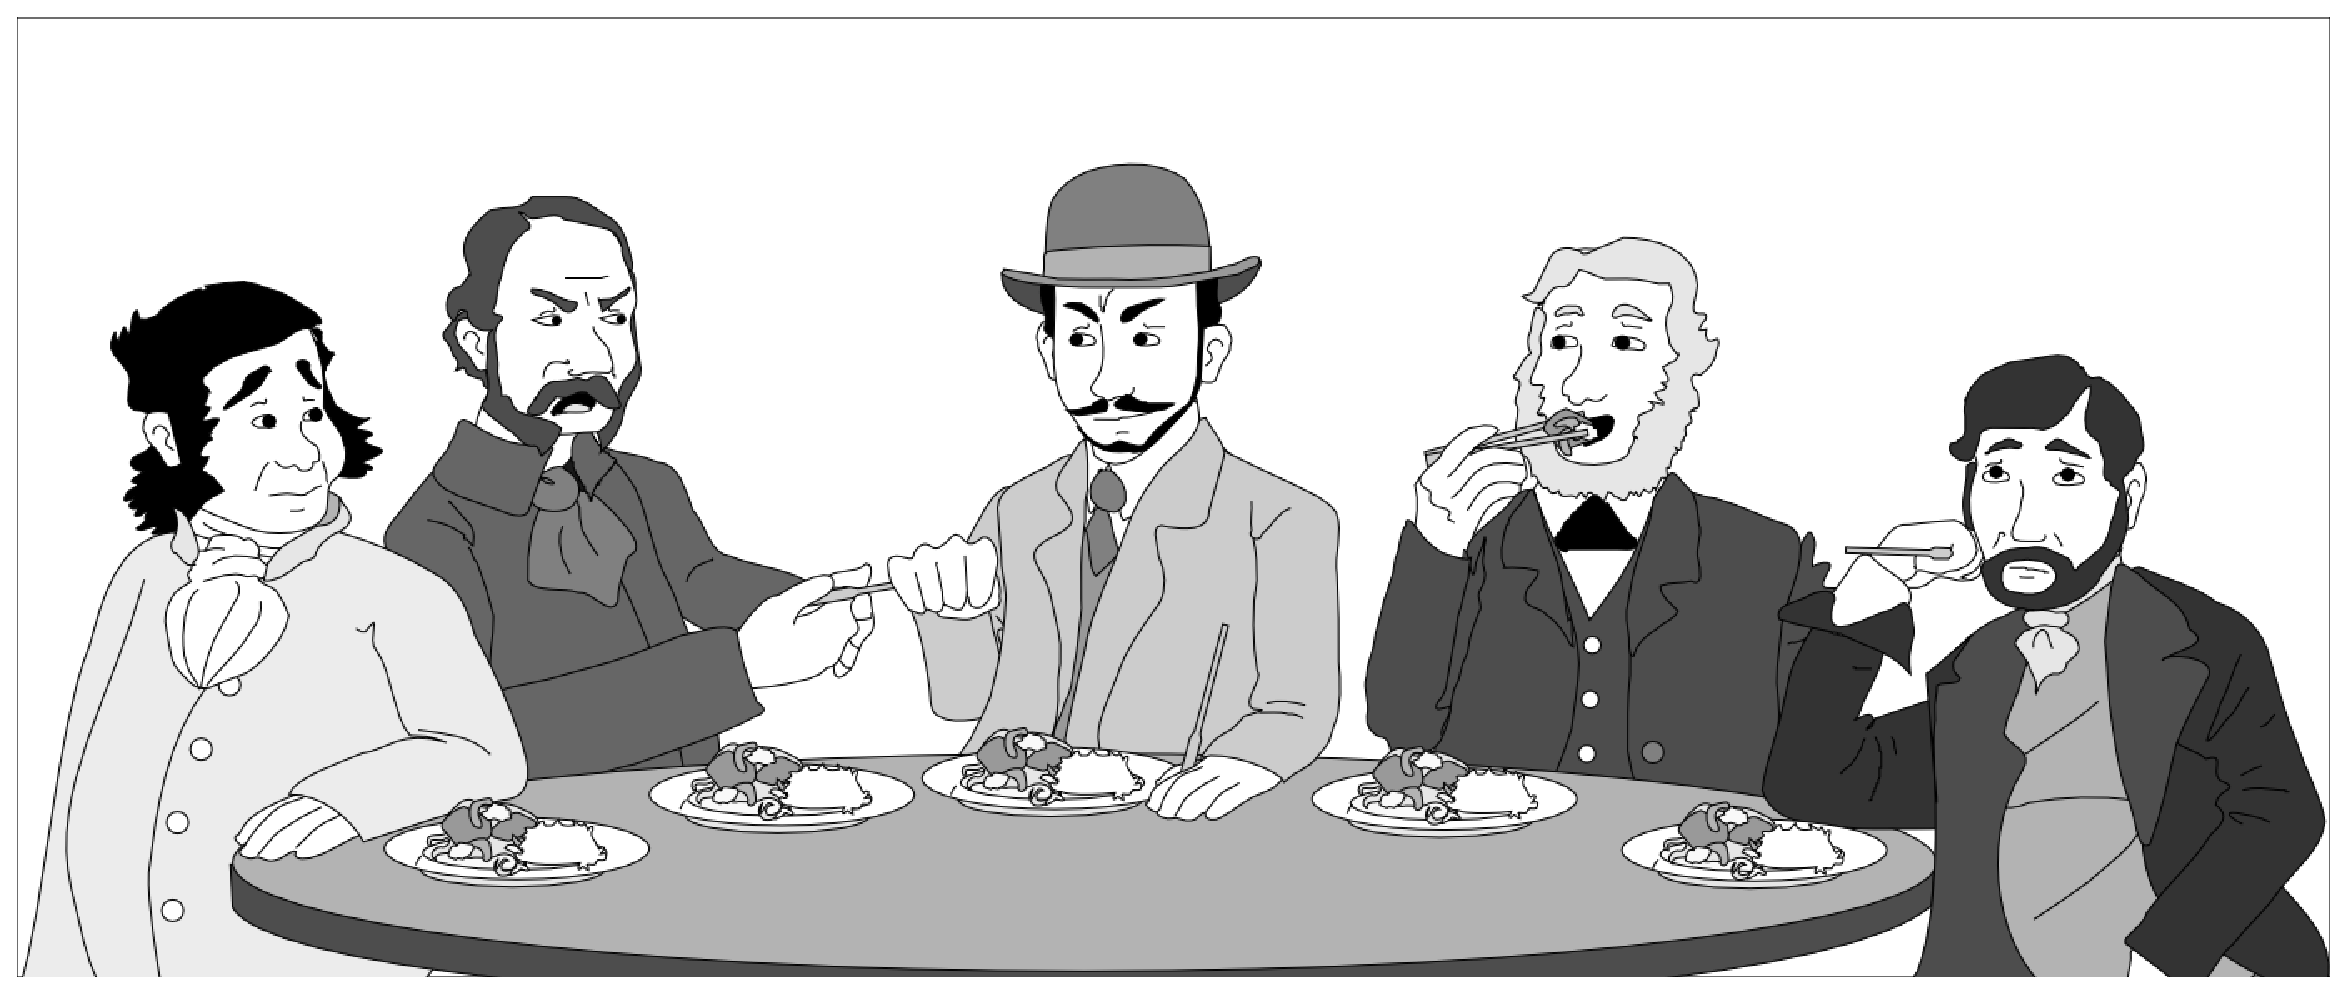
\includegraphics{cartoons/Dining-philosophers}}
\caption{Partial Starvation Is Also Bad}
\ContributedBy{Figure}{fig:cpu:Partial Starvation Is Also Bad}{Melissa Broussard}
\end{figure*}

목표는 말 그대로 기아를 방지할 수 있는 알고리즘을 만드는 것입니다.
가능한 한가지 기아 시나리오는 모든 철학자가 각자의 왼쪽 포크를 동시에 집어드는
경우입니다.
이들 중 누구도 그들이 식사를 끝내기 전까지는 자신의 포크를 내려놓지 않을
것이므로, 그리고 이들 중 누구도 이들 중 한명이라도 식사를 끝내기 전까지는
두번째 포크를 갖지 못할 것이므로, 이들은 모두 굶게 됩니다.
최소 한명의 철학자를 식사할 수 있게 하는 것만으로는 충분치 않음을 알아 두시기
바랍니다.
Figure~\ref{fig:cpu:Partial Starvation Is Also Bad} 가 보이듯, 오직 소수의
철학자가 기아에 빠지는 것조차도 방지되어야 합니다.

\iffalse

The object is to construct an algorithm that, quite literally,
prevents starvation.
One starvation scenario would be if all of the philosophers picked up
their leftmost forks simultaneously.
Because none of them will put down their fork until after they finished
eating, and because none of them may pick up their second fork until at
least one of them has finished eating, they all starve.
Please note that it is not sufficient to allow at least one philosopher
to eat.
As Figure~\ref{fig:cpu:Partial Starvation Is Also Bad}
shows, starvation of even a few of the philosophers is to be avoided.

\fi

\begin{figure}[tb]
\centering
\includegraphics[scale=.7]{SMPdesign/DiningPhilosopher5TB}
\caption{Dining Philosophers Problem, Textbook Solution}
\ContributedBy{Figure}{fig:SMPdesign:Dining Philosophers Problem, Textbook Solution}{Kornilios Kourtis}
\end{figure}

\pplsur{Edsger W.}{Dijkstra} 의 해결책은 1980년대 말 또는 1990년대 초에는
적절치 못하게 된, 무시할만한 통신 딜레이라는 가정을 적용하면 잘 동작하는 전역
세마포어를 사용했습니다.\footnote{
	2021년의 시각에서 Dijkstra 를 모욕하기는 너무도 쉽습니다, 50년이나 지난
	이야기니까요.
	여전히 Dijkstra 를 모욕해야 한다고 느끼신다면, 저는 무언가를 출판하고,
	50년을 기다린 후, \emph{여러분의} 아이디어가 그 시간동안의 시험을
	얼마나 잘 버텨냈는지 보라는 조언을 하겠습니다.}
보다 최신의 해결책은
Figure~\ref{fig:SMPdesign:Dining Philosophers Problem, Textbook Solution}
에 보인 것처럼 포크에 수를 매기는 것입니다.
각 철학자는 그 또는 그녀의 접시 옆에 있는 더 낮은 수를 가지는 포크를 집고,
그다음 다음 포크를 집습니다.
따라서, 이 그림에서 가장 위쪽에 앉은 철학자는 왼쪽 포크를 먼저 집어들고, 이어서
오른쪽 포크를 집어드는데, 나머지 철학자들은 각자의 오른쪽 포크를 먼저
집어듭니다.
두명의 철학자들이 포크~1 을 먼저 집어들려고 노력할 것이므로, 그리고 이 두
철학자들 중 한명만이 성공할 것이므로, 네명의 철학자에게 다섯개의 포크가 사용
가능하게 될 겁니다.
이 네명의 철학자 중 최소 한명은 두개의 포크를 가지게 될거고 따라서 식사를 할 수
있습니다.

\iffalse

\pplsur{Edsger W.}{Dijkstra}'s solution used a global semaphore,
which works fine assuming
negligible communications delays, an assumption that became invalid
in the late 1980s or early 1990s.\footnote{
	It is all too easy to denigrate Dijkstra from the viewpoint
	of the year 2021, more than 50 years after the fact.
	If you still feel the need to denigrate Dijkstra, my advice
	is to publish something, wait 50 years, and then see
	how well \emph{your} ideas stood the test of time.}
More recent solutions number the forks as shown in
Figure~\ref{fig:SMPdesign:Dining Philosophers Problem, Textbook Solution}.
Each philosopher picks up the lowest-numbered fork next to his or her
plate, then picks up the other fork.
The philosopher sitting in the uppermost position in the diagram thus
picks up the leftmost fork first, then the rightmost fork, while the
rest of the philosophers instead pick up their rightmost fork first.
Because two of the philosophers will attempt to pick up fork~1 first,
and because only one of those two philosophers will succeed,
there will be five forks available to four philosophers.
At least one of these four will have two forks, and will thus be able
to eat.

\fi

이 자원에 숫자를 매기고 그 숫자 순서대로 자원을 획득하는 일반적인 기법은 데드락
방지 기법으로 널리 사용되었습니다.
하지만, 모두가 배고픈데 한번에 단 한명의 철학자만이 식사를 하는 상황이 초래되는
사건의 연속을 쉽게 상상해 볼 수 있습니다:

\begin{enumerate}
    \item P2 가 포크~1 을 집어들어, P1 이 포크를 집는 걸 방지합니다.
    \item P3 가 포크~2 를 집어듭니다.
    \item P4 가 포크~3 를 집어듭니다.
    \item P5 가 포크~4 를 집어듭니다.
    \item P5 가 포크~5 를 집어들고 식사를 합니다.
    \item P5 가 포크~4 와~5 를 내려놓습니다.
    \item P4 가 포크~4 를 집어들고 식사를 합니다.
\end{enumerate}

요약하자면, 이 알고리즘은 동시에 두 철학자가 식사를 하기 충분한 것 이상의
포크가 존재함에도 불구하고 모든 철학자가 배고플 때에도 한번에 하나의 철학자만
식사를 하는 상황을 초래할 수 있습니다.
이보다 더 잘할 수 있어야 합니다!

\iffalse

This general technique of numbering resources and acquiring them in
numerical order is heavily used as a deadlock-prevention technique.
However, it is easy to imagine a sequence of events that will result
in only one philosopher eating at a time even though all are hungry:

\begin{enumerate}
    \item P2 picks up fork~1, preventing P1 from taking a fork.
    \item P3 picks up fork~2.
    \item P4 picks up fork~3.
    \item P5 picks up fork~4.
    \item P5 picks up fork~5 and eats.
    \item P5 puts down forks~4 and~5.
    \item P4 picks up fork~4 and eats.
\end{enumerate}

In short, this algorithm can result in only one philosopher eating at
a given time, even when all five philosophers are hungry,
despite the fact that there are more than enough forks for two
philosophers to eat concurrently.
It should be possible to do better than this!

\fi

\begin{figure}[tb]
\centering
\includegraphics[scale=.7]{SMPdesign/DiningPhilosopher4part-b}
\caption{Dining Philosophers Problem, Partitioned}
\ContributedBy{Figure}{fig:SMPdesign:Dining Philosophers Problem, Partitioned}{Kornilios Kourtis}
\end{figure}

한가지 해결책이
Figure~\ref{fig:SMPdesign:Dining Philosophers Problem, Partitioned}
에 그려져 있는데, 이 파티셔닝 기법을 더 잘 보이기 위해 다섯명이 아닌 네명의
철학자만 포함하고 있습니다.
여기서 위쪽과 오른쪽의 철학자들은 한쌍의 포크를 공유하며, 아래쪽과 왼쪽의
철학자는 다른 한쌍의 포크를 공유합니다.
만약 모든 철학자들이 동시에 배고파지면, 최소 두명은 항상 동시에 식사를 할 수
있습니다.
또한, 그림에 보여져 있듯이, 이 포크들은 이제 한쌍으로 묶여있을 수 있어서 두개씩
동시에 집어지고 내려놓아질 수 있게 되어, 획득과 해제 알고리즘을 단순화
시킵니다.

\iffalse

One approach is shown in
Figure~\ref{fig:SMPdesign:Dining Philosophers Problem, Partitioned},
which includes four philosophers rather than five to better illustrate the
partition technique.
Here the upper and rightmost philosophers share a pair of forks,
while the lower and leftmost philosophers share another pair of forks.
If all philosophers are simultaneously hungry, at least two will
always be able to eat concurrently.
In addition, as shown in the figure, the forks can now be bundled
so that the pair are picked up and put down simultaneously, simplifying
the acquisition and release algorithms.

\fi

\QuickQuiz{
	이 Dining Philosophers 문제에 더 나은 해결책이 있을까요?

	\iffalse

	Is there a better solution to the Dining
	Philosophers Problem?

	\fi

}\QuickQuizAnswer{
	그런 향상된 해결책 하나가
	Figure~\ref{fig:SMPdesign:Dining Philosophers Problem, Fully Partitioned}
	에 보여져 있는데, 단순히 철학자들에게 추가의 다섯개 포크를 제공하는
	것입니다.
	모든 다섯명의 철학자가 이제 동시에 식사를 할 수 있고, 어떤 철학자도
	다른 누군가를 기다릴 필요가 없습니다.
	또한, 이 방법은 무척 향상된 재앙 통제를 제공합니다.

	\iffalse

	One such improved solution is shown in
	Figure~\ref{fig:SMPdesign:Dining Philosophers Problem, Fully Partitioned},
	where the philosophers are simply provided with an additional
	five forks.
	All five philosophers may now eat simultaneously, and there
	is never any need for philosophers to wait on one another.
	In addition, this approach offers greatly improved disease control.

	\fi

\begin{figure}[tb]
\centering
\includegraphics[scale=.7]{SMPdesign/DiningPhilosopher5PEM}
\caption{Dining Philosophers Problem, Fully Partitioned}
\QContributedBy{Figure}{fig:SMPdesign:Dining Philosophers Problem, Fully Partitioned}{Kornilios Kourtis}
\end{figure}

	이 해결책은 누군가에겐 속임수처럼 보일 수도 있겠습니다만, 이런 종류의
	``속임수'' 가 많은 동시성 문제에 있어 좋은 해결책을 찾기 위한
	열쇠입니다.

	\iffalse

	This solution might seem like cheating to some, but such
	``cheating'' is key to finding good solutions to many
	concurrency problems.

	\fi

}\QuickQuizEnd

이는 ``수평 병렬성''~\cite{Inman85} 또는 ``데이터 병렬성'' 의 한 예로, 이
철학자들 쌍 간에는 어떤 의존성이 없기 때문에 그렇게 이름지어졌습니다.
수평적으로 병렬인 데이터 처리 시스템에서, 데이터의 특정 항목은 복사된
소프트웨어 컴포넌트들 중 하나에 의해서만 처리될 겁니다.

\iffalse

This is an example of ``horizontal parallelism''~\cite{Inman85}
or ``data parallelism'',
so named because there is no dependency among the pairs of philosophers.
In a horizontally parallel data-processing system, a given item of data
would be processed by only one of a replicated set of software
components.

\fi

\QuickQuiz{
	그리고 어떤 의미에서 이 ``수평적 병렬성'' 은 ``수평적'' 이라고 불릴 수
	있는 건가요?

	\iffalse

	And in just what sense can this ``horizontal parallelism'' be
	said to be ``horizontal''?

	\fi

}\QuickQuizAnswer{
	Inman 은 일반적으로 어플리케이션이 꼭대기에, 그리고 하드웨어 연결부가
	바닥에, 수직으로 그려지는 프로토콜 스택을 가지고 일하고 있었습니다.
	데이터는 이 스택의 위에서 아래로 흐릅니다.
	``수평적 병렬성'' 은 패킷을 다른 네트워크 연결부로부터 병렬로 처리하는
	반면, ``수직 병렬성'' 은 주어진 패킷을 다른 프로토콜 처리 단계로 동시에
	처리합니다.

	``수직 병렬성'' 은 또한 ``파이프라이닝'' 이라고도 불립니다.

	\iffalse

	Inman was working with protocol stacks, which are normally
	depicted vertically, with the application on top and the
	hardware interconnect on the bottom.
	Data flows up and down this stack.
	``Horizontal parallelism'' processes packets from different network
	connections in parallel, while ``vertical parallelism''
	handles different protocol-processing steps for a given
	packet in parallel.

	``Vertical parallelism'' is also called ``pipelining''.

	\fi

}\QuickQuizEnd

\subsection{Double-Ended Queue}
\label{sec:SMPdesign:Double-Ended Queue}

Double-ended queue 는 양 끝을 통해 추가되거나 제거될 수 있는 원소들의 리스트를
갖는 데이터 구조입니다~\cite{Knuth73}.
락 기반의 구현으로는 double-ended queue 의 양 끝단에서의 동시적 운용이
어려움으로 알려져 있습니다~\cite{DanGrossman2007TMGCAnalogy}.
이 섹션은 파티셔닝 설계 전략이 어떻게 합리적으로 간단한 구현에 이르게 할 수
있는지 보이고, 뒤따르는 섹션들에서는 세개의 범용 접근법을 봅니다.

\iffalse

A double-ended queue is a data structure containing a list of elements
that may be inserted or removed from either end~\cite{Knuth73}.
It has been claimed that a lock-based implementation permitting
concurrent operations on both ends of the double-ended queue is
difficult~\cite{DanGrossman2007TMGCAnalogy}.
This section shows how a partitioning design strategy can result
in a reasonably simple implementation, looking at three
general approaches in the following sections.

\fi

\subsubsection{Left- and Right-Hand Locks}
\label{sec:SMPdesign:Left- and Right-Hand Locks}

\begin{figure}[tb]
\centering
\resizebox{3in}{!}{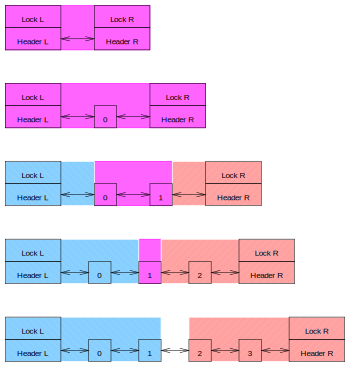
\includegraphics{SMPdesign/lockdeq}}
\caption{Double-Ended Queue With Left- and Right-Hand Locks}
\label{fig:SMPdesign:Double-Ended Queue With Left- and Right-Hand Locks}
\end{figure}

간단해 보이는 한가지 전략은 왼쪽 끝으로의 enqueue 와 dequeue 오퍼레이션을 위한
왼쪽 락과 오른쪽 끝으로의 오퍼레이션들을 위한 오른쪽 락을 갖는 doubly linked
list 를 사용하는 것으로,
Figure~\ref{fig:SMPdesign:Double-Ended Queue With Left- and Right-Hand Locks}
에 보이는 것과 같습니다.
하지만, 이 방법의 문제는 이 리스트에 네개 미만의 원소만이 존재할 때에는 이 두
락의 도메인이 겹친다는 것입니다.
이 겹침은 어떤 원소를 제거하는 것이 그 원소만이 아니라 그것의 왼쪽과 오른쪽
이웃 원소에게도 영향을 끼친다는 사실 때문입니다.
이 도메인들은 이 그림에 색깔로 표시되어 있는데, 아래쪽으로의 줄무늬를 가진
파랑은 왼쪽 락의 도메인을, 위쪽으로의 줄무늬를 가진 빨강은 오른쪽 락의
도메인을, 그리고 (줄무늬가 없는) 보라색은 겹치는 도메인을 표시합니다.
이 방식으로 동작하는 알고리즘을 만드는 것도 가능하지만, 다섯개 미만이 아닌 특수
경우들이 존재한다는 사실은 커다랗고 빨간 경고등을 띄우는데, 이 리스트의 다른
끝쪽에서의 동시의 행동들이 이 queue 를 언제든 하나의 특수 경우에서 다른 경우로
바꿀 수 있다는 점에서 특히 그렇습니다.
다른 설계를 고려하는 게 훨씬 나을 겁니다.

\iffalse

One seemingly straightforward approach would be to use a doubly
linked list with a left-hand lock
for left-hand-end enqueue and dequeue operations along with a right-hand
lock for right-hand-end operations, as shown in
Figure~\ref{fig:SMPdesign:Double-Ended Queue With Left- and Right-Hand Locks}.
However, the problem with this approach is that the two locks'
domains must overlap when there are fewer than four elements on the
list.
This overlap is due to the fact that removing any given element affects
not only that element, but also its left- and right-hand neighbors.
These domains are indicated by color in the figure, with blue
with downward stripes indicating
the domain of the left-hand lock, red with upward stripes
indicating the domain of the right-hand
lock, and purple (with no stripes) indicating overlapping domains.
Although it is possible to create an algorithm that works this way,
the fact that it has no fewer than five special cases should raise
a big red flag, especially given that concurrent activity at the other
end of the list can shift the queue from one special case to another
at any time.
It is far better to consider other designs.

\fi

\subsubsection{Compound Double-Ended Queue}
\label{sec:SMPdesign:Compound Double-Ended Queue}

\begin{figure}[tb]
\centering
\resizebox{3in}{!}{\includegraphics{SMPdesign/lockdeqpair}}
\caption{Compound Double-Ended Queue}
\label{fig:SMPdesign:Compound Double-Ended Queue}
\end{figure}

겹치지 않는 락 도메인을 강제하기 위한 한가지 방법이
Figure~\ref{fig:SMPdesign:Compound Double-Ended Queue}
에 보여져 있습니다.
두개의 double-ended queue 들이 동시에 동작하는데, 각각 자신의 락으로
보호됩니다.
이는 원소들이 결국은 한쪽 double-ended queue 에서 다른 쪽으로 옮겨져야 하며,
이때는 양쪽 락이 모두 잡혀야만 함을 의미합니다.
데드락을 방지하기 위해 간단한 락 계층이 사용될 수 있는데, 예를 들면 오른쪽 락을
잡기 전에 항상 왼쪽 락을 잡는 겁니다.
이러면 우리는 조건 없이 왼쪽 queue 에 원소를 왼쪽 집어넣기하고 오른쪽 queue 에
원소를 오른쪽 집어넣기를 할 수 있으므로, 같은 double-ended queue 에 두개의 락을
적용하는 것보다는 훨씬 간단할 것입니다.
비어있는 queue 에서 꺼내기를 하려 할 때 주요한 복잡도가 나타나는데, 이 경우에는
다음과 같은 처리가 필요합니다:

\iffalse

One way of forcing non-overlapping lock domains is shown in
Figure~\ref{fig:SMPdesign:Compound Double-Ended Queue}.
Two separate double-ended queues are run in tandem, each protected by
its own lock.
This means that elements must occasionally be shuttled from one of
the double-ended queues to the other, in which case both locks must
be held.
A simple lock hierarchy may be used to avoid deadlock, for example,
always acquiring the left-hand lock before acquiring the right-hand lock.
This will be much simpler than applying two locks to the same
double-ended queue, as we can unconditionally left-enqueue elements
to the left-hand queue and right-enqueue elements to the right-hand
queue.
The main complication arises when dequeuing from an empty queue, in
which case it is necessary to:

\fi

\begin{enumerate}
\item	오른쪽 락을 잡고 있다면, 이를 해제하고 왼쪽 락을 잡습니다.
\item	오른쪽 락을 잡습니다.
\item	두 queue 에 원소를 고르게 분배시킵니다.
\item	제거하려는 원소가 있다면 제거합니다.
\item	두 락을 모두 해제합니다.

\iffalse

\item	If holding the right-hand lock, release it and acquire the
	left-hand lock.
\item	Acquire the right-hand lock.
\item	Rebalance the elements across the two queues.
\item	Remove the required element if there is one.
\item	Release both locks.

\fi

\end{enumerate}

\QuickQuiz{
	이 compound double-ended queue 구현에서는, 이 락을 해제하고 재획득 하는
	동안에 이 queue 가 비어있지 않게 되면 어떡해야 하죠?

	\iffalse

	In this compound double-ended queue implementation, what should
	be done if the queue has become non-empty while releasing
	and reacquiring the lock?

	\fi

}\QuickQuizAnswer{
	이 경우에는, 그냥 이 비어있지 않은 큐에서 원소를 제거하고, 두 락을
	해제하고, 리턴하면 됩니다.

	\iffalse

	In this case, simply dequeue an item from the non-empty
	queue, release both locks, and return.

	\fi

}\QuickQuizEnd

이 결과로 나오는 코드는 (\path{locktdeq.c}) 상당히 간단합니다.
원소 재분배 오퍼레이션은 주어진 원소를 두 queue 사이에서 어느 쪽으로든 옮길
수도 있어서, 시간을 낭비하고, 최적의 성능을 위해선 워크로드 종속적 휴리스틱을
필요로 할 수도 있습니다.
이게 어떤 경우에는 최선의 방법이 될수도 있겠습니다만, 알고리즘을 더 큰 결정성을
가지고 시도해 보는것도 흥미로울 겁니다.

\iffalse

The resulting code (\path{locktdeq.c}) is quite straightforward.
The rebalancing operation might well shuttle a given element back
and forth between the two queues, wasting time and possibly requiring
workload-dependent heuristics to obtain optimal performance.
Although this might well be the best approach in some cases, it is
interesting to try for an algorithm with greater determinism.

\fi

\subsubsection{Hashed Double-Ended Queue}
\label{sec:SMPdesign:Hashed Double-Ended Queue}

데이터 구조를 결정론적으로 쪼개는 가장 효과적이고도 가장 간단한 방법은
해싱입니다.
각 원소에 이 리스트에서의 그것의 위치에 기반한 숫자를 부여해서 비어있는 queue
에 왼쪽으로 들어온 첫번째 원소는 0으로 수가 부여되고 비어있는 queue 에
오른쪽으로 들어온 첫번째 원소는 1이라는 수가 부여되는 식으로 double-ended
queue 를 간단히 해싱하는게 가능합니다.
왼쪽으로 들어오는 원소들은 계속해서 작아지는 수를 부여받고 ($-1$, $-2$, $-3$,
\ldots), 오른쪽으로 들어오는 원소들은 계속해서 증가하는 수를 부여받습니다 (2,
3, 4, \ldots).
핵심은, 이 숫자가 이 queue 에서의 위치를 암시하므로, 해당 원소의 수를 정말로
표현할 필요는 없다는 겁니다.

\iffalse

One of the simplest and most effective ways to deterministically
partition a data structure is to hash it.
It is possible to trivially hash a double-ended queue by assigning
each element a sequence number based on its position in the list,
so that the first element left-enqueued into an empty queue is numbered
zero and the first element right-enqueued into an empty queue is numbered
one.
A series of elements left-enqueued into an otherwise-idle queue would
be assigned decreasing numbers ($-1$, $-2$, $-3$, \ldots), while a series of
elements right-enqueued into an otherwise-idle queue would be assigned
increasing numbers (2, 3, 4, \ldots).
A key point is that it is not necessary to actually represent a given
element's number, as this number will be implied by its position in
the queue.

\fi

\begin{figure}[tb]
\centering
\resizebox{3in}{!}{\includegraphics{SMPdesign/lockdeqhash}}
\caption{Hashed Double-Ended Queue}
\label{fig:SMPdesign:Hashed Double-Ended Queue}
\end{figure}

이 방법에서는, 우리는 왼쪽 인덱스를 보호하기 위해 하나의 락을 할당하고, 오른쪽
인덱스를 위해 또다른 락을, 그리고 각 해쉬 체인을 위해 또하나의 락을 사용합니다.
Figure~\ref{fig:SMPdesign:Hashed Double-Ended Queue} 가 네개의 해쉬 체인이
있다는 가정 하에 이로 인해 만들어지는 데이터 구조를 보입니다.
락 도메인은 겹치지 않으며, 데드락은 체인 락 전에 인덱스 락을 획득함으로써
회피되며, 특정 타입의 (인덱스 또는 체인) 락은 한번에 두개 이상 획득하지
않습니다.

\iffalse

Given this approach, we assign one lock to guard the left-hand index,
one to guard the right-hand index, and one lock for each hash chain.
Figure~\ref{fig:SMPdesign:Hashed Double-Ended Queue} shows the resulting
data structure given four hash chains.
Note that the lock domains do not overlap, and that deadlock is avoided
by acquiring the index locks before the chain locks, and by never
acquiring more than one lock of a given type (index or chain) at a time.

\fi

\begin{figure}[tb]
\centering
\resizebox{3in}{!}{
\includegraphics{SMPdesign/lockdeqhash1R}}
\caption{Hashed Double-Ended Queue After Insertions}
\label{fig:SMPdesign:Hashed Double-Ended Queue After Insertions}
\end{figure}

각 해쉬 체인은 그 자체로 double-ended queue 이며, 이 예에서는 각각이 네개의
원소씩을 쥐고 있습니다.
Figure~\ref{fig:SMPdesign:Hashed Double-Ended Queue After Insertions}
의 가장 위쪽은 하나의 원소가 (``R$_1$'') 오른쪽으로 넣어지고, 해쉬 체인~2 를
참조하게끔 증가된 오른쪽 인덱스를 갖게 된 후의 상태를 보입니다.
이 그림의 가운데 부분은 세개의 원소가 추가적으로 오른쪽으로 넣어진 후의 상태를
보입니다.
보시다시피, 인덱스들은 각자의 초기 상태로 되돌아가져 있습니다
(Figure~\ref{fig:SMPdesign:Hashed Double-Ended Queue}를 보세요), 하지만 각 해시
체인은 이제 비어 있습니다.
이 그림의 아래쪽은 세개의 추가적인 원소가 왼쪽으로 들어오고 또하나의 원소가
오른쪽으로 들어온 후의 상태를 보입니다.

Figure~\ref{fig:SMPdesign:Hashed Double-Ended Queue After Insertions} 에 보인
마지막 상태로부터, 왼쪽 dequeue 오퍼레이션은 원소 ``L$_{-2}$'' 를 리턴하고,
왼쪽 인덱스가 해쉬 체인~2 를 참조하는대로 둘 것이며, 이 체인은 단 하나의
원소만을 (``R$_2$'') 가지고 있게 됩니다.
이 상태에서, 왼쪽 enqueue 가 오른쪽 enqueue 와 동시에 수행되면 락 경쟁이 발생할
겁니다만, 그런 경쟁 상태의 확률은 더 큰 해쉬 테이블을 사용함으로써 무척 낮은
수준으로 줄일 수 있습니다.

\iffalse

Each hash chain is itself a double-ended queue, and in this example,
each holds every fourth element.
The uppermost portion of
Figure~\ref{fig:SMPdesign:Hashed Double-Ended Queue After Insertions}
shows the state after a single element (``R$_1$'') has been
right-enqueued, with the right-hand index having been incremented to
reference hash chain~2.
The middle portion of this same figure shows the state after
three more elements have been right-enqueued.
As you can see, the indexes are back to their initial states
(see Figure~\ref{fig:SMPdesign:Hashed Double-Ended Queue}), however,
each hash chain is now non-empty.
The lower portion of this figure shows the state after three additional
elements have been left-enqueued and an additional element has been
right-enqueued.

From the last state shown in
Figure~\ref{fig:SMPdesign:Hashed Double-Ended Queue After Insertions},
a left-dequeue operation would return element ``L$_{-2}$'' and leave
the left-hand index referencing hash chain~2, which would then
contain only a single element (``R$_2$'').
In this state, a left-enqueue running concurrently with a right-enqueue
would result in lock contention, but the probability of such contention
can be reduced to arbitrarily low levels by using a larger hash table.

\fi

\begin{figure}[tb]
\centering
\resizebox{1.5in}{!}{
\includegraphics{SMPdesign/lockdeqhashlots}}
\caption{Hashed Double-Ended Queue With 16 Elements}
\label{fig:SMPdesign:Hashed Double-Ended Queue With 16 Elements}
\end{figure}

Figure~\ref{fig:SMPdesign:Hashed Double-Ended Queue With 16 Elements}
는 16개의 원소가 네개 해쉬 버킷 기반의 병렬 double-ended queue 에 어떻게 관리될
지 보입니다.
아랫단의 단일 락 기반 double-ended queue 각각은 전체 병렬 double-ended queue 의
1/4 조각을 갖습니다.

\iffalse

Figure~\ref{fig:SMPdesign:Hashed Double-Ended Queue With 16 Elements}
shows how 16 elements would be organized in a four-hash-bucket
parallel double-ended queue.
Each underlying single-lock double-ended queue holds a one-quarter
slice of the full parallel double-ended queue.

\fi

\begin{listing}[tbp]
\input{CodeSamples/SMPdesign/lockhdeq@struct_pdeq.fcv}
\caption{Lock-Based Parallel Double-Ended Queue Data Structure}
\label{lst:SMPdesign:Lock-Based Parallel Double-Ended Queue Data Structure}
\end{listing}

Listing~\ref{lst:SMPdesign:Lock-Based Parallel Double-Ended Queue Data Structure}
은 평범하게 락으로 관리되는 double-ended-queue 구현을 제공하는 \co{struct deq}
가 존재한다는 가정 하에 앞에서 이야기한 것에 연관되는 C-언어 데이터 구조를
보입니다.
\begin{fcvref}[ln:SMPdesign:lockhdeq:struct_pdeq]
이 데이터 구조는 라인~\lnref{llock} 에 왼쪽 락을, 라인~\lnref{lidx} 에 왼쪽
인덱스를, 라인~\lnref{rlock} 에 오른쪽 락을 (실제 구현에서는 캐쉬라인 사이즈로
정렬된), 라인~\lnref{ridx} 에 오른쪽 인덱스를, 그리고 마지막으로,
라인~\lnref{bkt} 에 간단한 락 기반 double-ended queue 의 배열을 가지고
있습니다.
고성능 구현체는 거짓 공유를 피하기 위해 패딩이나 특수한 정렬 지시어 등을 사용할
겁니다.
\end{fcvref}

\iffalse

Listing~\ref{lst:SMPdesign:Lock-Based Parallel Double-Ended Queue Data Structure}
shows the corresponding C-language data structure, assuming an
existing \co{struct deq} that provides a trivially locked
double-ended-queue implementation.
\begin{fcvref}[ln:SMPdesign:lockhdeq:struct_pdeq]
This data structure contains the left-hand lock on line~\lnref{llock},
the left-hand index on line~\lnref{lidx}, the right-hand lock on line~\lnref{rlock}
(which is cache-aligned in the actual implementation),
the right-hand index on line~\lnref{ridx}, and, finally, the hashed array
of simple lock-based double-ended queues on line~\lnref{bkt}.
A high-performance implementation would of course use padding or special
alignment directives to avoid false sharing.
\end{fcvref}

\fi

\begin{listing}[tbp]
\input{CodeSamples/SMPdesign/lockhdeq@pop_push.fcv}
\caption{Lock-Based Parallel Double-Ended Queue Implementation}
\label{lst:SMPdesign:Lock-Based Parallel Double-Ended Queue Implementation}
\end{listing}

Listing~\ref{lst:SMPdesign:Lock-Based Parallel Double-Ended Queue Implementation}
(\path{lockhdeq.c})
은 enqueue 와 dequeue 함수의 구현을 보입니다.\footnote{
	어떤 언어를 사용해서든 다양한 형태의 구현을 만들 수 있겠습니다만, 그건
	독자 여러분의 연습 문제로 남겨 두겠습니다.}
이야기는 왼쪽 오퍼레이션들에 집중할텐데, 오른쪽 오퍼레이션들은 쉽게 왼쪽의
것들로부터 나올 것이기 때문입니다.

\begin{fcvref}[ln:SMPdesign:lockhdeq:pop_push:popl]
\Clnrefrange{b}{e} 는 왼쪽 dequeue 를 하고 가능하면 원소를, 그렇지 않다면
\co{NULL} 을 리턴하는 \co{pdeq_pop_l()} 을 보입니다.
라인~\lnref{acq} 는 왼쪽 스핀락을 획득하고, 라인~\lnref{idx} 는 dequeue 될
인덱스를 계산합니다.
라인~\lnref{deque} 는 이 원소를 꺼내고, 라인~lnref{check} 에서 이 결과가
\co{NULL} 이 아닐 것으로 판명되면, 라인~\lnref{rel} 에서 락을 해제하고,
마지막으로 라인~\lnref{return} 에서 거기 원소가 있었다면 그것을, 아니면
\co{NULL} 을 리턴합니다.
\end{fcvref}

\iffalse

Listing~\ref{lst:SMPdesign:Lock-Based Parallel Double-Ended Queue Implementation}
(\path{lockhdeq.c})
shows the implementation of the enqueue and dequeue functions.\footnote{
	One could easily create a polymorphic implementation in any
	number of languages, but doing so is left as an exercise for
	the reader.}
Discussion will focus on the left-hand operations, as the right-hand
operations are trivially derived from them.

\begin{fcvref}[ln:SMPdesign:lockhdeq:pop_push:popl]
\Clnrefrange{b}{e} show \co{pdeq_pop_l()},
which left\-/dequeues and returns
an element if possible, returning \co{NULL} otherwise.
Line~\lnref{acq} acquires the left-hand spinlock,
and line~\lnref{idx} computes the
index to be dequeued from.
Line~\lnref{deque} dequeues the element, and,
if line~\lnref{check} finds the result to be
non-\co{NULL}, line~\lnref{record} records the new left-hand index.
Either way, line~\lnref{rel} releases the lock, and,
finally, line~\lnref{return} returns
the element if there was one, or \co{NULL} otherwise.
\end{fcvref}

\fi

\begin{fcvref}[ln:SMPdesign:lockhdeq:pop_push:pushl]
\Clnrefrange{b}{e} 는 특정 원소를 왼쪽으로 enqueue 하는 \co{pdeq_push_l()} 을
보입니다.
라인~\lnref{acq} 는 왼쪽 락을 획득하고, 라인~\lnref{idx} 에서 왼쪽 인덱스를
잡습니다.
라인~\lnref{enque} 는 이 원소를 이 왼쪽 인덱스로 가리켜지는 double-ended queue
에 왼쪽으로 enqueue gkqslek.
라인~\lnref{update} 는 이어서 이 왼쪽 인덱스를 업데이트 하고 라인~\lnref{rel}
에서 이 락을 해제합니다.
\end{fcvref}

앞에서도 이야기 했듯, 오른쪽 오퍼레이션들은 왼쪽의 것들과 완전히 비슷하므로,
그것들의 분석은 독자 여러분의 연습 문제로 남겨 둡니다.

\iffalse

\begin{fcvref}[ln:SMPdesign:lockhdeq:pop_push:pushl]
\Clnrefrange{b}{e} show \co{pdeq_push_l()},
which left-enqueues the specified
element.
Line~\lnref{acq} acquires the left-hand lock,
and line~\lnref{idx} picks up the left-hand
index.
Line~\lnref{enque} left-enqueues the specified element
onto the double-ended queue
indexed by the left-hand index.
Line~\lnref{update} then updates the left-hand index
and line~\lnref{rel} releases the lock.
\end{fcvref}

As noted earlier, the right-hand operations are completely analogous
to their left-handed counterparts, so their analysis is left as an
exercise for the reader.

\fi

\QuickQuiz{
	해쉬 기반의 double-ended queue 는 좋은 해결책일까요?
	왜 그렇고 왜 그렇지 않을까요?

	\iffalse

	Is the hashed double-ended queue a good solution?
	Why or why not?

	\fi

}\QuickQuizAnswer{
	여기 답변하는 최선의 방법은 여러개의 다른 멀티프로세서 시스템에서
	\path{lockhdeq.c} 를 수행해 보는 것이며, 여러분이 가능한 시간 내에
	그렇게 할 것을 장려합니다.
	걱정을 할 수 있는 한가지 이유는 이 구현에서 각 오퍼레이션은 하나가 아닌
	두개의 락을 획득해야 한다는 것입니다.

	잘 설계된 첫번째 성능 연구가 예로 들어질 겁니다.\footnote{
		Dalessandro 등의
		연구~\cite{LukeDalessandro:2011:ASPLOS:HybridNOrecSTM:deque}
		와 Dice 등의 연구~\cite{DavidDice:2010:SCA:HTM:deque} 는 훌륭한
		시작 지점이 될 겁니다.}
	순차적 구현과의 비교도 잊지 마십시오!

	\iffalse

	The best way to answer this is to run \path{lockhdeq.c} on
	a number of different multiprocessor systems, and you are
	encouraged to do so in the strongest possible terms.
	One reason for concern is that each operation on this
	implementation must acquire not one but two locks.
	% Getting about 500 nanoseconds per element when used as
	% a queue on a 4.2GHz Power system.  This is roughly the same as
	% the version covered by a single lock.  Sequential (unlocked
	% variant is more than an order of magnitude faster!

	The first well-designed performance study will be cited.\footnote{
		The studies by Dalessandro
		et al.~\cite{LukeDalessandro:2011:ASPLOS:HybridNOrecSTM:deque}
		and Dice et al.~\cite{DavidDice:2010:SCA:HTM:deque} are
		excellent starting points.}
	Do not forget to compare to a sequential implementation!

	\fi

}\QuickQuizEnd

\subsubsection{Compound Double-Ended Queue Revisited}
\label{sec:SMPdesign:Compound Double-Ended Queue Revisited}

이 섹션은 조합된 double-ended queue 를 비어 있지 않은 queue 에서 이제 비어 있는
queue 로 모든 원소를 옮기는 간단한 균형 맞추기를 사용하는 방법으로 다시
풀어봅니다.

\iffalse

This section revisits the compound double-ended queue, using a trivial
rebalancing scheme that moves all the elements from the non-empty
queue to the now-empty queue.

\fi

\QuickQuiz{
	빈 queue 로 \emph{모든} 원소를 옮긴다구요?
	이 미친 해결책이 대체 어떤 세상에서는 최적인거죠???

	\iffalse

	Move \emph{all} the elements to the queue that became empty?
	In what possible universe is this brain-dead solution in any
	way optimal???

	\fi

}\QuickQuizAnswer{
	데이터 흐름의 방향이 가끔씩만 바뀌는 경우에 최적입니다.
	이 double-ended queue 가 동시에 양 끝에서 비워지는 경우엔 물론 무척
	안좋은 선택일 겁니다.
	이는 물론 다른 질문을 떠오르게 하는데, 양끝에서 동시에 비우기를 하는건
	대체 어떤 세상에서 합리적인 일이겠냐는 겁니다.
	이 질문에 대한 가능한 답 중 하나는 work stealing queue 입니다.

	\iffalse

	It is optimal in the case where data flow switches direction only
	rarely.
	It would of course be an extremely poor choice if the double-ended
	queue was being emptied from both ends concurrently.
	This of course raises another question, namely, in what possible
	universe emptying from both ends concurrently would be a reasonable
	thing to do.
	Work-stealing queues are one possible answer to this question.

	\fi

}\QuickQuizEnd

앞의 섹션에서 보인 해쉬 기반 구현과 대조적으로, 이 조합 구현은 락도 어토믹
오퍼레이션도 사용하지 않는 순차적 구현의 double-ended queue 위에서 구현될
겁니다.

\iffalse

In contrast to the hashed implementation presented in
the previous section, the compound implementation will build on
a sequential implementation of a double-ended queue that uses
neither locks nor atomic operations.

\fi

\begin{listing}[tbp]
\input{CodeSamples/SMPdesign/locktdeq@pop_push.fcv}
\caption{Compound Parallel Double-Ended Queue Implementation}
\label{lst:SMPdesign:Compound Parallel Double-Ended Queue Implementation}
\end{listing}

Listing~\ref{lst:SMPdesign:Compound Parallel Double-Ended Queue Implementation}
이 이 구현을 보이고 있습니다.
해쉬 기반의 구현과 달리, 이 조합 구현은 비대칭적이어서, \co{pdeq_pop_l()} 과
\co{pdeq_pop_r()} 구현을 별개로 봐야만 합니다.

\iffalse

Listing~\ref{lst:SMPdesign:Compound Parallel Double-Ended Queue Implementation}
shows the implementation.
Unlike the hashed implementation, this compound implementation is
asymmetric, so that we must consider the \co{pdeq_pop_l()}
and \co{pdeq_pop_r()} implementations separately.

\fi

\QuickQuiz{
	조합된 병렬 double-ended queue 구현은 왜 대칭적일 수 없죠?

	\iffalse

	Why can't the compound parallel double-ended queue
	implementation be symmetric?

	\fi

}\QuickQuizAnswer{
	락 계층을 사용해 데드락을 회피해야한다는 필요성이 비대칭성을
	강제하는데, 식사하는 철학자들 문제의 포크 번호 매기기 해결책과 같은
	것입니다
	(Section~\ref{sec:SMPdesign:Dining Philosophers Problem} 을
	참고하세요).

	\iffalse

	The need to avoid deadlock by imposing a lock hierarchy
	forces the asymmetry, just as it does in the fork-numbering
	solution to the Dining Philosophers Problem
	(see Section~\ref{sec:SMPdesign:Dining Philosophers Problem}).

	\fi

}\QuickQuizEnd

\begin{fcvref}[ln:SMPdesign:locktdeq:pop_push:popl]
\co{pdeq_pop_l()} 구현이 이 코드의 \clnrefrange{b}{e} 에 보여져 있습니다.
라인~\lnref{acq:l} 은 왼쪽 락을 획득하는데, 이 락은 라인~\lnref{rel:l} 에서
해제됩니다.
라인~\lnref{deq:ll} 은 아랫단의 double-ended queue 의 왼쪽으로부터 원소를
빼내려 시도하고, 이게 성공하면 간단히 이 원소를 리턴하기 위해
\clnrefrange{acq:r}{skip} 을 건너뜁니다.
그렇지 않다면, 라인~\lnref{acq:r} 은 오른쪽 락을 획득하고, 라인~\lnref{deq:lr}
에서 오른쪽 queue 로부터 원소를 왼쪽 꺼내기 하고 라인~\lnref{move} 에서 오른쪽
queue 의 모든 남아있는 원소를 왼쪽 queue 로 옮기며, 라인~\lnref{init:r} 에서
오른쪽 queue 를 초기화 하고, 라인~\lnref{rel:r} 에서 이 오른쪽 락을 해제합니다.
만약 존재한다면 라인~\lnref{deq:lr} 에서 dequeue 된 원소가 리턴됩니다.
\end{fcvref}

\iffalse

\begin{fcvref}[ln:SMPdesign:locktdeq:pop_push:popl]
The \co{pdeq_pop_l()} implementation is shown on
\clnrefrange{b}{e}
of the listing.
Line~\lnref{acq:l} acquires the left-hand lock,
which line~\lnref{rel:l} releases.
Line~\lnref{deq:ll} attempts to left-dequeue an element
from the left-hand underlying
double-ended queue, and, if successful,
skips \clnrefrange{acq:r}{skip} to simply
return this element.
Otherwise, line~\lnref{acq:r} acquires the right-hand lock, line~\lnref{deq:lr}
left-dequeues an element from the right-hand queue,
and line~\lnref{move} moves any remaining elements on the right-hand
queue to the left-hand queue, line~\lnref{init:r} initializes
the right-hand queue,
and line~\lnref{rel:r} releases the right-hand lock.
The element, if any, that was dequeued on line~\lnref{deq:lr} will be returned.
\end{fcvref}

\fi

\begin{fcvref}[ln:SMPdesign:locktdeq:pop_push:popr]
\co{pdeq_pop_r()} 구현이 이 코드의 \clnrefrange{b}{e} 에 보여져 있습니다.
전과 같이, 라인~\lnref{acq:r1} 은 이 오른쪽 락을 획득하고 (그리고
라인~\lnref{rel:r2} 에서 이를 해제합니다), 라인~\lnref{deq:rr1} 에서 오른쪽
queue 로부터 원소 하나를 오른쪽 꺼내기 하려 시도하고, 만약 성공한다면 이 원소를
단순히 리턴하기 위해 \clnrefrange{rel:r1}{skip2} 를 건너뜁니다.
하지만, 라인~\lnref{check1} 이 dequeue 할 원소가 존재하지 않았음을 알아내면
라인~\lnref{rel:r1} 은 이 오른쪽 락을 해제하고 \clnrefrange{acq:l}{acq:r2} 가
올바른 순서로 두 락을 잡습니다.
라인~\lnref{deq:rr2} 는 이제 오른쪽 queue 로부터 원소 하나를 다시 오른쪽 꺼내기
하려 시도하고, 라인~\lnref{check2} 가 이 두번째 시도가 실패했음을 확인하면,
라인~\lnref{deq:rl} 은 왼쪽 queue 로부터 원소 하나를 오른쪽 dequeue 하고
(원소가 있었다면), 라인~\lnref{move} 는 모든 남아있는 원소들을 왼쪽 queue
로부터 오른쪽 queue 로 옮기고, 라인~\lnref{init:l} 은 왼쪽 queue 를 초기화
합니다.
어떻게 되었든, 라인~\lnref{rel:l} 은 왼쪽 락을 해제합니다.
\end{fcvref}

\iffalse

\begin{fcvref}[ln:SMPdesign:locktdeq:pop_push:popr]
The \co{pdeq_pop_r()} implementation is shown on \clnrefrange{b}{e}
of the listing.
As before, line~\lnref{acq:r1} acquires the right-hand lock
(and line~\lnref{rel:r2}
releases it), and line~\lnref{deq:rr1} attempts to right-dequeue an element
from the right-hand queue, and, if successful,
skips \clnrefrange{rel:r1}{skip2}
to simply return this element.
However, if line~\lnref{check1} determines that there was no element to dequeue,
line~\lnref{rel:r1} releases the right-hand lock and
\clnrefrange{acq:l}{acq:r2} acquire both
locks in the proper order.
Line~\lnref{deq:rr2} then attempts to right-dequeue an element
from the right-hand
queue again, and if line~\lnref{check2} determines that this second attempt has
failed, line~\lnref{deq:rl} right-dequeues an element from the left-hand queue
(if there is one available), line~\lnref{move} moves any remaining elements
from the left-hand queue to the right-hand queue, and line~\lnref{init:l}
initializes the left-hand queue.
Either way, line~\lnref{rel:l} releases the left-hand lock.
\end{fcvref}

\fi

\QuickQuizSeries{%
\QuickQuizB{
	Listing~\ref{lst:SMPdesign:Compound Parallel Double-Ended Queue Implementation}
	의 라인~\ref{ln:SMPdesign:locktdeq:pop_push:popr:deq:rr2}
	에서의 오른쪽 dequeue 재시도가 왜 필요하죠?

	\iffalse

	Why is it necessary to retry the right-dequeue operation
	on line~\ref{ln:SMPdesign:locktdeq:pop_push:popr:deq:rr2} of
	Listing~\ref{lst:SMPdesign:Compound Parallel Double-Ended Queue Implementation}?

	\fi

}\QuickQuizAnswerB{
	\begin{fcvref}[ln:SMPdesign:locktdeq:pop_push:popr]
	이 쓰레드가 라인~\lnref{rel:r1} 에서 \co{d->rlock} 을 내려놓고
	라인~\lnref{acq:r2} 에서 이 락을 다시 획득하는 사이에 다른 쓰레드가
	원소를 하나 enqueue 했을 수도 있기 때문에 이 재시도가 필요합니다.
	\end{fcvref}

	\iffalse

	\begin{fcvref}[ln:SMPdesign:locktdeq:pop_push:popr]
	This retry is necessary because some other thread might have
	enqueued an element between the time that this thread dropped
	\co{d->rlock} on line~\lnref{rel:r1} and the time that it reacquired this
	same lock on line~\lnref{acq:r2}.
	\end{fcvref}

	\fi

}\QuickQuizEndB
%
\QuickQuizE{
	분명 왼쪽 락은 \emph{가끔은} 획득 가능할 거예요!!!
	그런데도 왜
	Listing~\ref{lst:SMPdesign:Compound Parallel Double-Ended Queue Implementation}
	의 라인~\ref{ln:SMPdesign:locktdeq:pop_push:popr:rel:r1}
	에서는 무조건적으로 오른쪽 락을 해제해야 하는 거죠?

	\iffalse

	Surely the left-hand lock must \emph{sometimes} be available!!!
	So why is it necessary that
        line~\ref{ln:SMPdesign:locktdeq:pop_push:popr:rel:r1} of
	Listing~\ref{lst:SMPdesign:Compound Parallel Double-Ended Queue Implementation}
	unconditionally release the right-hand lock?

	\fi

}\QuickQuizAnswerE{
	왼쪽 락을 획득 가능할 때 획득하기 위해서 \co{spin_trylock()} 을
	사용하는 것도 가능할 겁니다.
	하지만, 그 실패의 경우에는 여전히 이 오른쪽 락을 내려놓고 두 락을
	제대로 된 순서로 다시 획득해야 할 겁니다.
	이 변화를 만드는 것은 (그리고 이게 그럴 가치가 있는지 알아내는 것은)
	독자 여러분의 연습문제로 남겨두겠습니다.

	\iffalse

	It would be possible to use \co{spin_trylock()} to attempt
	to acquire the left-hand lock when it was available.
	However, the failure case would still need to drop the
	right-hand lock and then re-acquire the two locks in order.
	Making this transformation (and determining whether or not
	it is worthwhile) is left as an exercise for the reader.

	\fi

}\QuickQuizEndE
}

\begin{fcvref}[ln:SMPdesign:locktdeq:pop_push:pushl]
\co{pdeq_push_l()} 구현이
Listing~\ref{lst:SMPdesign:Compound Parallel Double-Ended Queue Implementation}
의 \clnrefrange{b}{e} 에 보여져 있습니다.
라인~\lnref{acq:l} 은 왼쪽 스핀락을 획득하고, 라인~\lnref{que:l} 은 이 원소를
왼쪽 큐에 왼쪽으로 집어넣고, 마지막으로 라인~\lnref{rel:l} 은 이 락을
해제합니다.
\end{fcvref}
\begin{fcvref}[ln:SMPdesign:locktdeq:pop_push:pushr]
\co{pdeq_push_r()} 구현은 (\clnrefrange{b}{e} 에 보여져 있습니다) 상당히
비슷합니다.
\end{fcvref}

\iffalse

\begin{fcvref}[ln:SMPdesign:locktdeq:pop_push:pushl]
The \co{pdeq_push_l()} implementation is shown on
\clnrefrange{b}{e} of
Listing~\ref{lst:SMPdesign:Compound Parallel Double-Ended Queue Implementation}.
Line~\lnref{acq:l} acquires the left-hand spinlock,
line~\lnref{que:l} left-enqueues the
element onto the left-hand queue, and finally line~\lnref{rel:l} releases
the lock.
\end{fcvref}
\begin{fcvref}[ln:SMPdesign:locktdeq:pop_push:pushr]
The \co{pdeq_push_r()} implementation (shown on \clnrefrange{b}{e})
is quite similar.
\end{fcvref}

\fi

\QuickQuiz{
	하지만 데이터가 한 방향으로만 흐르는 경우에,
	Listing~\ref{lst:SMPdesign:Compound Parallel Double-Ended Queue Implementation}
	에 보인 알고리즘은 마지막 원소를 가져가서 아랫단의 double-ended queue
	를 비울 때마다 양 끝단이 같은 락을 획득하려 할 겁니다.
	이는 이 알고리즘이 양 끝단으로 동시의 액세스를 제공하는 것이 이 queue
	가 상당히 큰 수의 원소를 가지고 있을 때조차 실패할 수 있음을 의미하지
	않나요?

	\iffalse

	But in the case where data is flowing in only one direction,
	the algorithm shown in
	Listing~\ref{lst:SMPdesign:Compound Parallel Double-Ended Queue Implementation}
	will have both ends attempting to acquire the same lock
	whenever the consuming end empties its underlying
	double-ended queue.
	Doesn't that mean that sometimes this algorithm fails to
	provide concurrent access to both ends of the queue even
	when the queue contains an arbitrarily large number of elements?

	\fi

}\QuickQuizAnswer{
	실제로 그렇습니다!

	하지만 같은 속성을 가지고 있다고 하는 다른 알고리즘들도 마찬가지입니다.
	예를 들어, 락들의 해쉬 배열을 사용하는 소프트웨어 트랜잭셔널 메모리
	메커니즘을 사용하는 해결책들에서는 가장 왼쪽과 가장 오른쪽 원소들의
	주소가 가끔은 같은 락에 해쉬되는 경우가 있을 겁니다.
	이런 해쉬 충돌 역시 동시의 액세스를 방지할 겁니다.
	다른 예를 하나 들어보자면, 소프트웨어 fallback 을 갖추고 하드웨어
	트랜잭셔널 메모리 메커니즘을 사용하는
	해결책에서는~\cite{Yoo:2013:PEI:2503210.2503232,RickMerrit2011PowerTM,ChristianJacobi2012MainframeTM}
	이 소프트웨어 fallback 내에서 락킹을 종종 사용할 것이고, 따라서 무엇이
	되었든 이 락킹 해결책이 겪는 한계만큼 한계를 겪을 겁니다 (비록 뜸하긴
	하길 바랍니다만).

	따라서 2021년 기준으로, compound double-ended queue 를 포함한 동시의
	double-ended queue 문제를 위한 모든 실용적 해결책은 적어도 어떤
	환경에서는 완전한 동시성을 제공하지 못합니다.

	\iffalse

	Indeed it does!

	But the same is true of other algorithms claiming this property.
	For example, in solutions using software transactional memory
	mechanisms based on hashed arrays of locks,
	the leftmost and rightmost elements' addresses will sometimes
	happen to hash to the same lock.
	These hash collisions will also prevent concurrent access.
	For another example, solutions using hardware transactional
	memory mechanisms with software
	fallbacks~\cite{Yoo:2013:PEI:2503210.2503232,RickMerrit2011PowerTM,ChristianJacobi2012MainframeTM}
	often use locking within those software fallbacks, and thus
	suffer (albeit hopefully rarely) from whatever concurrency
	limitations that these locking solutions suffer from.

	Therefore, as of 2021, all practical solutions to the
	concurrent double-ended queue problem fail to provide full
	concurrency in at least some circumstances, including the
	compound double-ended queue.

	\fi

}\QuickQuizEnd

\subsubsection{Double-Ended Queue Discussion}
\label{sec:SMPdesign:Double-Ended Queue Discussion}

이 compound 구현은
Section~\ref{sec:SMPdesign:Hashed Double-Ended Queue}
에서 보인 해쉬 기반 구현에 비해 약간 복잡합니다만, 여전히 간단합니다.
물론, 더 영리한 균형맞추기 방법은 더 복잡할 수 있겠습니다만, 여기 보인 이
간단한 방법은 소프트웨어 대체제에
비해서도~\cite{LukeDalessandro:2011:ASPLOS:HybridNOrecSTM:deque}, 심지어
하드웨어의 도움을 받는 알고리즘에 비해서도~\cite{DavidDice:2010:SCA:HTM:deque}
성능이 좋은 것으로 드러났습니다.
그러나, 이런 방법에 있어 우리가 바랄 수 있는 최선은 두배의 확장성으로, 최대
두개의 쓰레드가 dequeue 의 락을 동시에 잡고 있을 수 있기 때문입니다.
이 한계는 또한 Michael 의 compare-and-swap 기반의 것과
같은~\cite{DBLP:conf/europar/Michael03} non-blocking 동기화 기반의 알고리즘에도
적용됩니다.\footnote{
	이 논문은 특수한 double-compare-and-swap (DCAS) 인스트럭션이
	double-ended queue 의 lock-free 구현을 만드는 데 필요하지 않음을
	보였다는 점에서 흥미롭습니다.
	대신, 흔한 compare-and-swap (예: x86 cmpxchg) 으로도 충분합니다.}

\iffalse

The compound implementation is somewhat more complex than the
hashed variant presented in
Section~\ref{sec:SMPdesign:Hashed Double-Ended Queue},
but is still reasonably simple.
Of course, a more intelligent rebalancing scheme could be arbitrarily
complex, but the simple scheme shown here has been shown to
perform well compared to software
alternatives~\cite{LukeDalessandro:2011:ASPLOS:HybridNOrecSTM:deque}
and even compared to algorithms using hardware
assist~\cite{DavidDice:2010:SCA:HTM:deque}.
Nevertheless, the best we can hope for from such a scheme
is 2x scalability, as at most two threads can be holding the
dequeue's locks concurrently.
This limitation also applies to algorithms based on non-blocking
synchronization, such as the compare-and-swap-based dequeue algorithm of
Michael~\cite{DBLP:conf/europar/Michael03}.\footnote{
	This paper is interesting in that it showed that special
	double-compare-and-swap (DCAS) instructions are not needed
	for lock-free implementations of double-ended queues.
	Instead, the common compare-and-swap (e.g., x86 cmpxchg)
	suffices.}

\fi

\QuickQuiz{
	Double-ended queue 문제에는 왜 한개가 아니라 두개의 해결책이 있는 거죠?

	\iffalse

	Why are there not one but two solutions to the double-ended queue
	problem?

	\fi

}\QuickQuizAnswer{
	사실은 최소 세개의 해결책이 있습니다.
	Dominik Dingel 의 것인 그 세번째 해결책은 reader-writer 락킹을 흥미로운
	방식으로 사용하며, \path{lockrwdeq.c} 에서 찾을 수 있을 겁니다.

	\iffalse

	There are actually at least three.
	The third, by Dominik Dingel, makes interesting use of
	reader-writer locking, and may be found in \path{lockrwdeq.c}.

	\fi

}\QuickQuizEnd

사실, Dice 등에 의해 이야기된 것처럼~\cite{DavidDice:2010:SCA:HTM:deque},
동기화 되지 않은 싱글쓰레드 기반 double-ended queue 는 그들이 연구한 어떤 병렬
구현들보다도 상당히 성능이 좋습니다.
따라서, 핵심은 공유된 queue 에 enqueue, dequeue 하는 데에는 그 구현과 관계 없이
상당한 오버헤드가 있을 수 있다는 것입니다.
이는 Chapter~\ref{chp:Hardware and its Habits} 에서 이야기한 것들을 놓고 생각해
보면, 이 queue 의 엄격한 first-in-first-out (FIFO) 특성을 놓고 볼 때, 전혀
놀랍지 않을 겁니다.

\iffalse

In fact, as noted by Dice et al.~\cite{DavidDice:2010:SCA:HTM:deque},
an unsynchronized single-threaded double-ended queue significantly
outperforms any of the parallel implementations they studied.
Therefore, the key point is that there can be significant overhead enqueuing to
or dequeuing from a shared queue, regardless of implementation.
This should come as no surprise in light of the material in
Chapter~\ref{chp:Hardware and its Habits}, given the strict
first-in-first-out (FIFO) nature of these queues.

\fi

더 나아가서, 이 엄격한 FIFO queue 는 사실 사용자에게 보이는 \emph{linearization
point}~\cite{Herlihy:1990:LCC:78969.78972}\footnote{
	짧게 요약해서, linearization point 는 어떤 함수의 내에서 이 함수가
	영향을 만들어 냈다고 말할 수 있는 하나의 지점입니다.
	이 락 기반의 구현에서, linearization point 는 이 크리티컬 섹션 내의
	모든 곳이라고 할 수 있습니다.}
에 대해서만 엄격한 FIFO 이며 이 예제에서는 이 linearization point 가 락
크리티컬 섹션 내에 여럿 있습니다.
이 queue 들은 (예를 들어) 각 개별 오퍼레이션이 시작된 시점에 대해서는 엄격한
FIFO 가 아닙니다~\cite{AndreasHaas2012FIFOisnt}.
이는 동시성 프로그램에서는 엄격한 FIFO 특성이 전혀 가치 있지 않음을 의미하며,
실제로 Kirsch 등은 향상된 성능과 확장성을 제공하는 덜 엄격한 queue 를
선보였습니다~\cite{ChristophMKirsch2012FIFOisntTR}.\footnote{
	Nir Shavit 은 대략 같은 이유로 완화된 스택을
	만들었습니다~\cite{Shavit:2011:DSM:1897852.1897873}.
	이 상황은 어떤 사람들을 linearization point 는 이론가들에겐 유용하지만
	개발자들에겐 그렇지 않다고 믿게 만들고, 그런 자료 구조와 알고리즘의
	설계자들이 얼마나 그들의 사용자들의 실제 필요를 고려했을지 의심하게
	만듭니다.}
그렇게 이야기 했지만, 여러분이 여러분의 동시성 프로그램이 사용하는 모든
데이터를 하나의 queue 로 보낸다면, 여러분은 여러분의 전체 설계를 다시 생각해
봐야 합니다.

\iffalse

Furthermore, these strict FIFO queues are strictly FIFO only with
respect to
\emph{linearization points}~\cite{Herlihy:1990:LCC:78969.78972}\footnote{
	In short, a linearization point is a single point within a given
	function where that function can be said to have taken effect.
	In this lock-based implementation, the linearization points
	can be said to be anywhere within the critical section that
	does the work.}
that are not visible to the caller, in fact, in these examples,
the linearization points are buried in the lock-based critical
sections.
These queues are not strictly FIFO with respect to (say) the times at which
the individual operations started~\cite{AndreasHaas2012FIFOisnt}.
This indicates that the strict FIFO property is not all that valuable
in concurrent programs, and in fact, Kirsch et al.\ present less-strict
queues that provide improved performance and
scalability~\cite{ChristophMKirsch2012FIFOisntTR}.\footnote{
	Nir Shavit produced relaxed stacks for roughly the same
	reasons~\cite{Shavit:2011:DSM:1897852.1897873}.
	This situation leads some to believe that the linearization
	points are useful to theorists rather than developers, and
	leads others to wonder to what extent the designers of such
	data structures and algorithms were considering the needs
	of their users.}
All that said, if you are pushing all the data used by your concurrent
program through a single queue, you really need to rethink your
overall design.

\fi

\subsection{Partitioning Example Discussion}
\label{sec:SMPdesign:Partitioning Example Discussion}

The optimal solution to the dining philosophers problem given in
the answer to the Quick Quiz in
Section~\ref{sec:SMPdesign:Dining Philosophers Problem}
is an excellent example of ``horizontal parallelism'' or
``data parallelism''.
The synchronization overhead in this case is nearly (or even exactly)
zero.
In contrast, the double-ended
queue implementations are examples of ``vertical parallelism'' or
``pipelining'', given that data moves from one thread to another.
The tighter coordination required for pipelining in turn requires
larger units of work to obtain a given level of efficiency.

\QuickQuizSeries{%
\QuickQuizB{
	The tandem double-ended queue runs about twice as fast as
	the hashed double-ended queue, even when I increase the
	size of the hash table to an insanely large number.
	Why is that?
}\QuickQuizAnswerB{
	The hashed double-ended queue's locking design only permits
	one thread at a time at each end, and further requires
	two lock acquisitions for each operation.
	The tandem double-ended queue also permits one thread at a time
	at each end, and in the common case requires only one lock
	acquisition per operation.
	Therefore, the tandem double-ended queue should be expected to
	outperform the hashed double-ended queue.

	Can you create a double-ended queue that allows multiple
	concurrent operations at each end?
	If so, how?  If not, why not?
}\QuickQuizEndB
%
\QuickQuizE{
	Is there a significantly better way of handling concurrency
	for double-ended queues?
}\QuickQuizAnswerE{
	One approach is to transform the problem to be solved
	so that multiple double-ended queues can be used in parallel,
	allowing the simpler single-lock double-ended queue to be used,
	and perhaps also replace each double-ended queue with a pair of
	conventional single-ended queues.
	Without such ``horizontal scaling'', the speedup is limited
	to 2.0.
	In contrast, horizontal-scaling designs can achieve very large
	speedups, and are especially attractive if there are multiple threads
	working either end of the queue, because in this
	multiple-thread case the dequeue
	simply cannot provide strong ordering guarantees.
	After all, the fact that a given thread removed an item first
	in no way implies that it will process that item
	first~\cite{AndreasHaas2012FIFOisnt}.
	And if there are no guarantees, we may as well obtain the
	performance benefits that come with refusing to provide these
	guarantees.
	% about twice as fast as hashed version on 4.2GHz Power.

	Regardless of whether or not the problem can be transformed
	to use multiple queues, it is worth asking whether work can
	be batched so that each enqueue and dequeue operation corresponds
	to larger units of work.
	This batching approach decreases contention on the queue data
	structures, which increases both performance and scalability,
	as will be seen in
	Section~\ref{sec:SMPdesign:Synchronization Granularity}.
	After all, if you must incur high synchronization overheads,
	be sure you are getting your money's worth.

	Other researchers are working on other ways to take advantage
	of limited ordering guarantees in
	queues~\cite{ChristophMKirsch2012FIFOisntTR}.
}\QuickQuizEndE
}

These two examples show just how powerful partitioning can be in
devising parallel algorithms.
Section~\ref{sec:SMPdesign:Locking Granularity and Performance}
looks briefly at a third example, matrix multiply.
However, all three of these examples beg for more and better design
criteria for parallel programs, a topic taken up in the next section.


% SMPdesign/criteria.tex
% SPDX-License-Identifier: CC-BY-SA-3.0

\section{Design Criteria}
\label{sec:SMPdesign:Design Criteria}

최고의 성능과 확장성을 얻는 방법 중 하나는 달성 가능한 최고의 병렬 프로그램이
만들어 질 때까지 해킹을 계속하는 것입니다.
하지만, 여러분의 프로그램이 현미경으로 봐야할 정도로 작지 않은 한, 가능한 병렬
프로그램의 공간은 우주의 수명이라는 거대한 시간 동안에도 최고의 달성 가능한
프로그램에 이르기를 보장하지 못할 정도로 커다랗습니다.
그리고 또, ``달성 가능한 최고의 병렬 프로그램'' 이란 무엇일까요?
어쨌든, Section~\ref{sec:intro:Parallel Programming Goals} 에서는 성능, 생산성,
그리고 범용성의 세가지 병렬 프로그래밍 목표를 이야기 했고, 달성 가능한 최고의
병렬 프로그램은 생산성과 범용성에의 비용으로 다가올 확률이 큽니다.
프로그램이 너무 구식이 되기 전에 충분히 받아들여질만큼 좋은 병렬 프로그램
정도는 되도록 하기 위해, 우리는 설계 단계에서 높은 수준에서의 선택들을 할 수
있어야 합니다.
\iffalse

One way to obtain the best performance and scalability is to simply
hack away until you converge on the best possible parallel program.
Unfortunately, if your program is other than microscopically tiny,
the space of possible parallel programs is so huge
that convergence is not guaranteed in the lifetime of the universe.
Besides, what exactly is the ``best possible parallel program''?
After all, Section~\ref{sec:intro:Parallel Programming Goals}
called out no fewer than three parallel-programming goals of
performance, productivity, and generality,
and the best possible performance will likely come at a cost in
terms of productivity and generality.
We clearly need to be able to make higher-level choices at design
time in order to arrive at an acceptably good parallel program
before that program becomes obsolete.
\fi

하지만, 정말로 실제 세계의 설계를 하기 위해선 디자인 규범들이 필요한데, 이
섹션에서 다룰 것입니다.
실제 세계에서, 이 규범들은 종종 더 크거나 작은 정도에서 충돌하므로, 설계자들은
그로 인한 트레이드오프들을 잘 균형 맞춰야 합니다.

이 규범들은 그 자체로써 설계에 동작하는 ``힘''들로 생각될 수 있으며, 특히 이런
힘들 간의 좋은 트레이드오프들은 ``디자인 패턴''~\cite{Alexander79,GOF95} 이라
불릴 수 있을 것입니다.

세개의 병렬 프로그래밍 목표들을 얻기 위한 디자인 규범들은 속도 향상, 경쟁,
오버헤드, 읽기-쓰기 비율, 그리고 복잡도입니다:
\iffalse

However, more detailed design criteria are required to
actually produce a real-world design, a task taken up in this section.
This being the real world, these criteria often conflict to a
greater or lesser degree, requiring that the designer carefully
balance the resulting tradeoffs.

As such, these criteria may be thought of as the ``forces''
acting on the design, with particularly good tradeoffs between
these forces being called ``design patterns''~\cite{Alexander79,GOF95}.

The design criteria for attaining the three parallel-programming goals
are speedup,
contention, overhead, read-to-write ratio, and complexity:
\fi
\begin{description}
\item[Speedup:]  Section~\ref{sec:intro:Parallel Programming Goals} 에서
	이야기했듯, 성능이야말로 우리가 대부분의 시간을 할애해야 하는 곳이고
	병렬화를 해야 하는 문제입니다.
	속도 향상은 순차적 버전의 프로그램을 돌리는데 드는 시간 대비 병렬
	버전을 돌리는데 드는 시간 사이의 비율입니다.
\item[Contention:]  더 많은 CPU 들이 한 병렬 프로그램에 사용되면 그 프로그램에
	의해 CPU들이 바삐 일하게 될 것이고, 여분의 CPU들은 다른 CPU들과의
	경쟁으로 인해 유의미한 일을 하지 못하게 되어버립니다.
	이런 경쟁은 락 경쟁, 메모리 경쟁, 또는 다른 성능 문제 부분으로부터의
	것일 수도 있습니다.
\iffalse

\item[Speedup:]  As noted in
	Section~\ref{sec:intro:Parallel Programming Goals},
	increased performance is the major reason
	to go to all of the time and trouble
	required to parallelize it.
	Speedup is defined to be the ratio of the time required
	to run a sequential version of the program to the time
	required to run a parallel version.
\item[Contention:]  If more CPUs are applied to a parallel
	program than can be kept busy by that program,
	the excess CPUs are prevented from doing
	useful work by contention.
	This may be lock contention, memory contention, or a host
	of other performance killers.
\fi
\item[Work-to-Synchronization Ratio:]  유니프로세서, 싱글쓰레드, preemption
	불가, 그리고 인터럽트 불가\footnote{
		인터럽트 마스킹을 하거나 그것들을 감지하지 못해서.}
	한 버전의 병렬 프로그램은 어떤 동기화 도구들도 필요가 없을 겁니다.
	따라서, 이런 도구들 (커뮤니케이션 캐시 미스, 메세지 응답시간, 락킹
	도구, 어토믹 인스트럭션들, 그리고 메모리 배리어 등) 에 의해 소모되는
	시간은 프로그램이 완수하려 의도한 유용한 일에 직접적으로 도움을 주지
	않는 오버헤드일 뿐입니다.
	중요하게 측정해 봐야 할 것은 동기화 오버헤드와 크리티컬 섹션 코드의
	오버헤드 사이의 관계로, 더 큰 크리티컬 섹션은 더 큰 동기화 오버헤드를
	정당화 시킴을 알아두시기 바랍니다.
	일 대비 동기화 비율은 동기화 효율성과 연관됩니다.
\iffalse

\item[Work-to-Synchronization Ratio:]  A uniprocessor,
	single\-/threaded, non-preemptible, and non\-/interruptible\footnote{
		Either by masking interrupts or by being oblivious to them.}
	version of a given parallel
	program would not need any synchronization primitives.
	Therefore, any time consumed by these primitives
	(including communication cache misses as well as
	message latency, locking primitives, atomic instructions,
	and memory barriers)
	is overhead that does not contribute directly to the useful
	work that the program is intended to accomplish.
	Note that the important measure is the
	relationship between the synchronization overhead
	and the overhead of the code in the critical section, with larger
	critical sections able to tolerate greater synchronization overhead.
	The work-to-synchronization ratio is related to
	the notion of synchronization efficiency.
\fi
\item[Read-to-Write Ratio:]  아주 가끔만 업데이트 되는 데이터 구조체는
	분할되기보다는 복제가 될 수 있을 것이고, 더 나아가서 쓰는 쪽에 부담을
	주는 대신 읽는 쪽의 동기화 오버헤드를 완화시켜주는 비대칭적 동기화
	도구를 사용해서 보호하는 식으로 전체 동기화 오버헤드를 줄일 수 있을
	것입니다.
	관련된 최적화들은 Chapter~\ref{chp:Counting} 에서 이야기 되었듯 자주
	업데이트 되는 데이터 구조체에도 적용될 수 있습니다.
\iffalse

\item[Read-to-Write Ratio:]  A data structure that is
	rarely updated may often be replicated rather than partitioned,
	and furthermore may be protected with asymmetric
	synchronization primitives that reduce readers' synchronization
	overhead at the expense of that of writers, thereby
	reducing overall synchronization overhead.
	Corresponding optimizations are possible for frequently
	updated data structures, as discussed in
	Chapter~\ref{chp:Counting}.
\fi
\item[Complexity:]  병렬 프로그램은 똑같은 일을 하는 순차적 프로그램에 비해
	복잡한데, 병렬 프로그램은 순차적 프로그램에 비해 훨씬 큰 상태 공간을
	갖기 때문입니다만, 충분한 질서와 구조가 주어진다면 이 상태 공간도 쉽게
	이해될 수 있긴 합니다.
	병렬 프로그램을 만드는 사람은 이 커다란 상태 공간의 문맥에서 동기화
	도구들, 메세지, 락킹 설계, 크리티컬 섹션 식별, 그리고 데드락을 고려해야
	합니다.

	이 거대한 복잡도는 종종 높은 개발 / 유지 비용으로 변환됩니다.
	따라서, 예산의 제한이 존재하는 프로그램에서는 가할 수 있는 변경의 수와
	종류를 제한할 수 있는데, 속도 향상은 많은 시간과 문제를 개선할 때에만
	가치가 있기 때문입니다.
	더 나쁜 것은, 추가된 복잡도가 실제로 성능과 확장성을 \emph{줄일} 수
	있다는 것입니다.

	따라서, 어떤 특정한 지점 이후부터는 병렬화보다는 더 싸고 효과적인
	순차적 최적화가 잠재하고 있을 수 있습니다.
	Section~\ref{sec:intro:Performance} 에서 이야기 했듯, 병렬화는 많은
	성능 최적화 방법 중 하나일 뿐이고, 더 나아가서 CPU 기반 병목 문제에
	적용될 수 있는 최적화입니다.
\iffalse

\item[Complexity:]  A parallel program is more complex than
	an equivalent sequential program because the parallel
	program has a much larger state space than does the
	sequential program, although these larger state spaces
	can in some cases be easily understood given sufficient
	regularity and structure.
	A parallel programmer must
	consider synchronization primitives, messaging, locking design,
	critical-section identification,
	and deadlock in the context of this larger state space.

	This greater complexity often translates
	to higher development and maintenance costs.
	Therefore, budgetary constraints can
	limit the number and types of modifications made to
	an existing program, since a given degree of speedup is
	worth only so much time and trouble.
	Worse yet, added complexity can actually \emph{reduce}
	performance and scalability.

	Therefore, beyond a certain point,
	there may be potential sequential optimizations
	that are cheaper and more effective than parallelization.
	As noted in
	Section~\ref{sec:intro:Performance},
	parallelization is but one performance optimization of
	many, and is furthermore an optimization that applies
	most readily to CPU-based bottlenecks.
\fi
\end{description}
이런 규범들은 최대의 속도향상을 위해 함께 동작할 것입니다.
앞의 세개의 규범들은 깊게 관계되어 있으므로, 이 섹션의 뒷부분은 이 상호관계에
대해 분석해 보겠습니다.\footnote{
	실제 세계의 병렬 시스템은 많은 디자인 규범들에 반하는 사례가 있을
	것인데, 데이터 구조체 레이아웃, 메모리 사이즈, 메모리 구조 대기시간,
	대역폭 제한, I/O 문제등이 그것입니다.}
\iffalse

These criteria will act together to enforce a maximum speedup.
The first three criteria are deeply interrelated, so
the remainder of this section analyzes these
interrelationships.\footnote{
	A real-world parallel system will be subject to many additional
	design criteria, such as data-structure layout,
	memory size, memory-hierarchy latencies, bandwidth limitations,
	and I/O issues.}
\fi

이런 규범들은 또한 요구사항의 일부분으로 나타날 수도 있음을 알아 두십시오.
예를 들어, 속도 향상은 상대적 요구사항으로 (``더 빠르게, 더 좋게'') 나올 수도
있고 워크로드의 절대적 요구사항으로 (``시스템은 최소한 초당 1,000,000 웹 힛을
지원해야 한다'') 나올 수도 있습니다.
고전의 디자인 패턴 언어들은 상대적 요구사항을 효력으로, 그리고 절대적
요구사항을 문맥으로 이야기 합니다.

이 디자인 규범들 사이의 관계에 대한 이해는 병렬 프로그램을 위한 적절한 설계
트레이드오프를 정하는 데에 많은 도움이 될 수 있을 겁니다.
\iffalse

Note that these criteria may also appear as part of the requirements
specification.
For example, speedup may act as a relative desideratum
(``the faster, the better'')
or as an absolute requirement of the workload (``the system
must support at least 1,000,000 web hits per second'').
Classic design pattern languages describe relative desiderata as forces
and absolute requirements as context.

An understanding of the relationships between these design criteria can
be very helpful when identifying appropriate design tradeoffs for a
parallel program.
\fi
\begin{enumerate}
\item	프로그램이 크리티컬 섹션들에서 더 적은 시간을 보낼수록, 잠재적인 속도
	향상은 커집니다.
	이는 Amdhal 의 법칙~\cite{GeneAmdahl1967AmdahlsLaw} 과, 주어진 시간
	동안 크리티컬 섹션은 오로지 하나의 CPU 에서만 실행될 수 있다는 사실로
	인한 결과입니다.

	더 자세히 이야기 하자면, 특정한 갯수의 CPU 들에서 실제 성능 향상을 얻기
	위해선, 프로그램이 배타적 크리티컬 섹션에서 소모하는 시간의 비율은 CPU
	들의 수의 역수보다 작아야 합니다.
	예를 들어, 10 개의 CPU 들을 사용하는 프로그램은 잘 확장하기 위해선 가장
	제한적인 크리티컬 섹션에서 자신의 전체 시간 중 10분의 1 미만을 사용해야
	합니다.
\item	경쟁은 많은 CPU 그리고/또는 실제 시간을 소모할 것이어서 실제 성능
	향상은 사용 가능한 CPU 들의 수보다 작을 겁니다.
	CPU 들의 수와 실제 속도 향상 사이의 차이가 클수록, CPU 들은 더
	비효율적으로 사용될 겁니다.
	유사하게, 원하는 효율성이 클수록 얻을 수 있는 속도 향상은 줄어들
	겁니다.
\iffalse

\item	The less time a program spends in critical sections,
	the greater the potential speedup.
	This is a consequence of Amdahl's Law~\cite{GeneAmdahl1967AmdahlsLaw}
	and of the fact that only one CPU may execute within a given
	critical section at a given time.

	More specifically, the fraction of time that the program spends in
	a given exclusive critical section must be much less than
	the reciprocal of the number of CPUs for the
	actual speedup to approach the number of CPUs.
	For example, a program running on 10 CPUs must spend
	much less than one tenth of its time in the most-restrictive
	critical section if it is to scale at all well.
\item	Contention effects will consume the excess CPU and/or
	wallclock time should the actual speedup be less than
	the number of available CPUs.  The
	larger the gap between the number of CPUs
	and the actual speedup, the less efficiently the
	CPUs will be used.
	Similarly, the greater the desired efficiency, the smaller
	the achievable speedup.
\fi
\item	사용 가능한 동기화 도구들이 그것들이 지키는 크리티컬 섹션들에 비해 높은
	오버헤드를 갖는다면, 속도 향상을 개선하는 최선의 방법은 그 도구들이
	사용되는 횟수를 줄이는 것입니다 (크리티컬 섹션들을 합치거나, 데이터
	소유권을 사용하거나, 비대칭적으로 도구를
	사용하거나(Section~\ref{chp:Deferred Processing} 을 참고하세요), 코드
	락킹과 같이 더 큰 단위를 사용하는 디자인 으로 옮겨가거나 하는
	방법으로).
\item	만약 크리티컬 섹션들이 그것들을 지키는 도구들에 비해 높은 오버헤드를
	갖는다면, 속도 향상을 개선하는 최선의 방법은 reader/writer 락킹, 데이터
	락킹, 비대칭적, 또는 데이터 소유권을 사용하는 쪽으로 옮겨가서 병렬성을
	높이는 것입니다.
\item	크리티컬 섹션들이 그것들을 지키는 도구들에 비해 높은 오버헤드를 갖고
	보호되는 데이터 구조체에는 수정보다 읽기가 훨씬 많이 수행된다면,
	병렬성을 높이는 최고의 방법은 reader/writer 락킹이나 비대칭적 도구들을
	사용하는 것입니다.
\item	SMP 성능을 개선하는 많은 변경들, 예를 들어 락 경쟁을 줄이는 것은 실시간
	응답시간도 향상시킵니다~\cite{PaulMcKenney2005h}.
\iffalse

\item	If the available synchronization primitives have
	high overhead compared to the critical sections
	that they guard, the best way to improve speedup
	is to reduce the number of times that the primitives
	are invoked (perhaps by batching critical sections,
	using data ownership, using asymmetric primitives
	(see Section~\ref{chp:Deferred Processing}),
	or by moving toward a more coarse-grained design
	such as code locking).
\item	If the critical sections have high overhead compared
	to the primitives guarding them, the best way
	to improve speedup is to increase parallelism
	by moving to reader/writer locking, data locking, asymmetric,
	or data ownership.
\item	If the critical sections have high overhead compared
	to the primitives guarding them and the data structure
	being guarded is read much more often than modified,
	the best way to increase parallelism is to move
	to reader/writer locking or asymmetric primitives.
\item	Many changes that improve SMP performance, for example,
	reducing lock contention, also improve real-time
	latencies~\cite{PaulMcKenney2005h}.
\fi
\end{enumerate}

\QuickQuiz{}
	크리티컬 섹션과 관련한 이 모든 문제들은 우리가 크리티컬 섹션이 아예
	없는 non-blocking 동기화~\cite{MauriceHerlihy90a}를 사용해야 한다는
	의미는 아닌가요?
	\iffalse

	Don't all these problems with critical sections mean that
	we should just always use
	non-blocking synchronization~\cite{MauriceHerlihy90a},
	which don't have critical sections?
	\fi
\QuickQuizAnswer{
	Non-blocking 동기화는 일부 상황에서는 매우 유용할 수 있지만,
	만병통치약은 아닙니다.
	또한, non-blocking 동기화는 Josh Triplett 에 의해 이야기되었듯 실제로는
	크리티컬 섹션을 갖습니다.
	예를 들어, compare-and-swap 오퍼레이션에 기반한 한 non-blocking
	알고리즘에서, 최초의 로드로 시작해 compare-and-swap 으로 이어지는
	코드는 여러면에서 락 기반의 크리티컬 섹션과 유사합니다.
	\iffalse

	Although non-blocking synchronization can be very useful
	in some situations, it is no panacea.
	Also, non-blocking synchronization really does have
	critical sections, as noted by Josh Triplett.
	For example, in a non-blocking algorithm based on
	compare-and-swap operations, the code starting at the
	initial load and continuing to the compare-and-swap
	is in many ways analogous to a lock-based critical section.
	\fi
} \QuickQuizEnd


\section{Synchronization Granularity}
\label{sec:SMPdesign:Synchronization Granularity}

\begin{figure}[tb]
\begin{center}
\includegraphics{SMPdesign/LockGranularity}
\end{center}
\caption{Design Patterns and Lock Granularity}
\label{fig:SMPdesign:Design Patterns and Lock Granularity}
\end{figure}

Figure~\ref{fig:SMPdesign:Design Patterns and Lock Granularity} 는 서로 다른
동기화 빈도의 단계를 그림으로 보여주는데, 각각의 단계는 뒤의 섹션에서 다루어질
것입니다.
이 섹션들은 주로 락킹에 중점을 맞춥니다만, 비슷한 빈도 문제가 모든 동기화
문제에 깔려 있습니다.
\iffalse

Figure~\ref{fig:SMPdesign:Design Patterns and Lock Granularity}
gives a pictorial view of different levels of synchronization granularity,
each of which is described in one of the following sections.
These sections focus primarily on locking, but similar granularity
issues arise with all forms of synchronization.
\fi

\subsection{Sequential Program}
\label{sec:SMPdesign:Sequential Program}

프로그램이 싱글 프로세서 위에서 충분히 빨리 돌아간다면, 그리고 다른
프로세스들이나 쓰레드, 또는 인터럽트 핸들러들과의 상호작용이 없다면, 동기화
기능들을 모두 제거해서 그것들의 오버헤드와 복잡성을 당신으로부터 떼어놓기
바랍니다.
몇년 전에는, Moore 의 법칙이 결국은 모든 프로그램을 이 카테고리로 만들 것이라
주장하던 사람들도 있었습니다.
하지만,
% @@@ Intel Trademark
Figure~\ref{fig:SMPdesign:Clock-Frequency Trend for Intel CPUs} 에서 볼 수
있듯이, 싱글 쓰레드의 성능의 기하급수적인 증가는 2003년 정도에 멈췄습니다.
따라서, 성능을 늘리기 위해선 병렬성을 필요로 할 것입니다.\footnote{
	이 그림은 이론적으로 클락당 하나 이상의 인스트럭션들을 처리할 수 있는
	최신 CPU 들의 경우 클락 주파수를, 그리고 하나의 간단한 인스트럭션을
	처리하는데 여러 클락을 필요로 하는 오래된 CPU 들의 경우 MIPS 를
	보입니다.
	이런 접근을 취하는 이유는 클락당 여러 인스트럭션들을 처리하는 최신 CPU
	들의 기능들은 일반적으로 메모리 시스템 성능에 제한되기 때문입니다.}
이 새로운 트렌드가 수천개의 CPU 들을 갖는 하나의 칩을 나타나게 할 것인지에 대한
논쟁은 금방 끝나지 않겠지만, Paul 이 이 문장을 듀얼코어 랩탑으로 쓰고 있다는
점을 볼 때, SMP 의 시대는 우리에게 와 있는 것으로 보입니다.
이더넷 대역폭이
Figure~\ref{fig:SMPdesign:Ethernet Bandwidth vs. Intel x86 CPU Performance}
에서 볼 수 있듯이 지속적으로 성장하고 있음을 알아두는 것 역시 중요합니다.
이런 추세는 커뮤니케이션 부하를 처리하기 위해 멀티쓰레드 서버들이 나타나도록
촉진하는 역할을 할 것입니다.
\iffalse

If the program runs fast enough on a single processor, and
has no interactions with other processes, threads, or interrupt
handlers, you should
remove the synchronization primitives and spare yourself their
overhead and complexity.
Some years back, there were those who would argue that Moore's Law
would eventually force all programs into this category.
However,
% @@@ Intel Trademark
as can be seen in
Figure~\ref{fig:SMPdesign:Clock-Frequency Trend for Intel CPUs},
the exponential increase in single-threaded performance halted in
about 2003.
Therefore,
increasing performance will increasingly require parallelism.\footnote{
	This plot shows clock frequencies for newer CPUs theoretically
	capable of retiring one or more instructions per clock, and MIPS for
	older CPUs requiring multiple clocks to execute even the
	simplest instruction.
	The reason for taking this approach is that the newer CPUs'
	ability to retire multiple instructions per clock is typically
	limited by memory-system performance.}
The debate as to whether this new trend will result in single chips
with thousands
of CPUs will not be settled soon, but given that Paul is typing this
sentence on a dual-core laptop, the age of SMP does seem to be upon us.
It is also important to note that Ethernet bandwidth is continuing
to grow, as shown in
Figure~\ref{fig:SMPdesign:Ethernet Bandwidth vs. Intel x86 CPU Performance}.
This growth will motivate multithreaded servers in order to handle
the communications load.
\fi

\begin{figure}[htb]
\begin{center}
\resizebox{3in}{!}{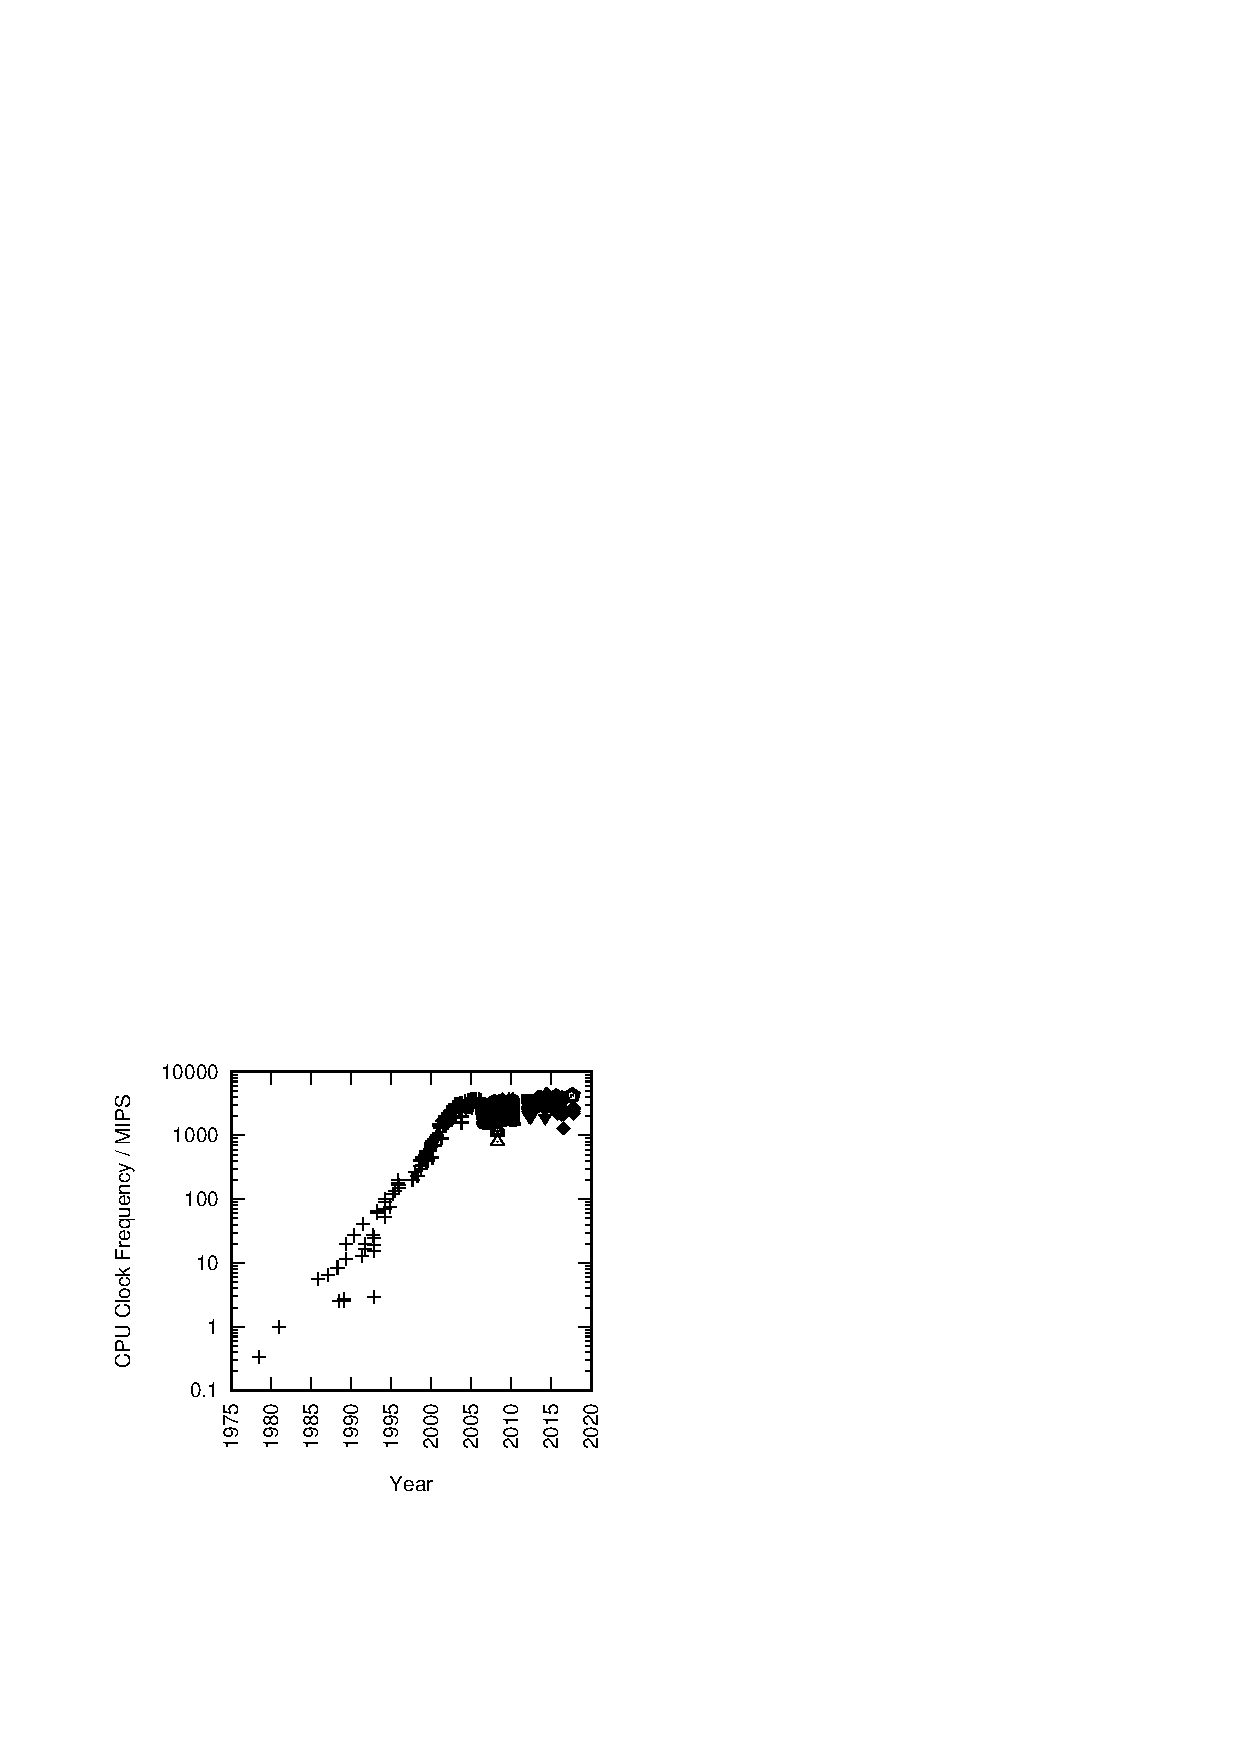
\includegraphics{SMPdesign/clockfreq}}
\end{center}
\caption{MIPS/Clock-Frequency Trend for Intel CPUs}
\label{fig:SMPdesign:Clock-Frequency Trend for Intel CPUs}
\end{figure}

\begin{figure}[htb]
\begin{center}
\resizebox{3in}{!}{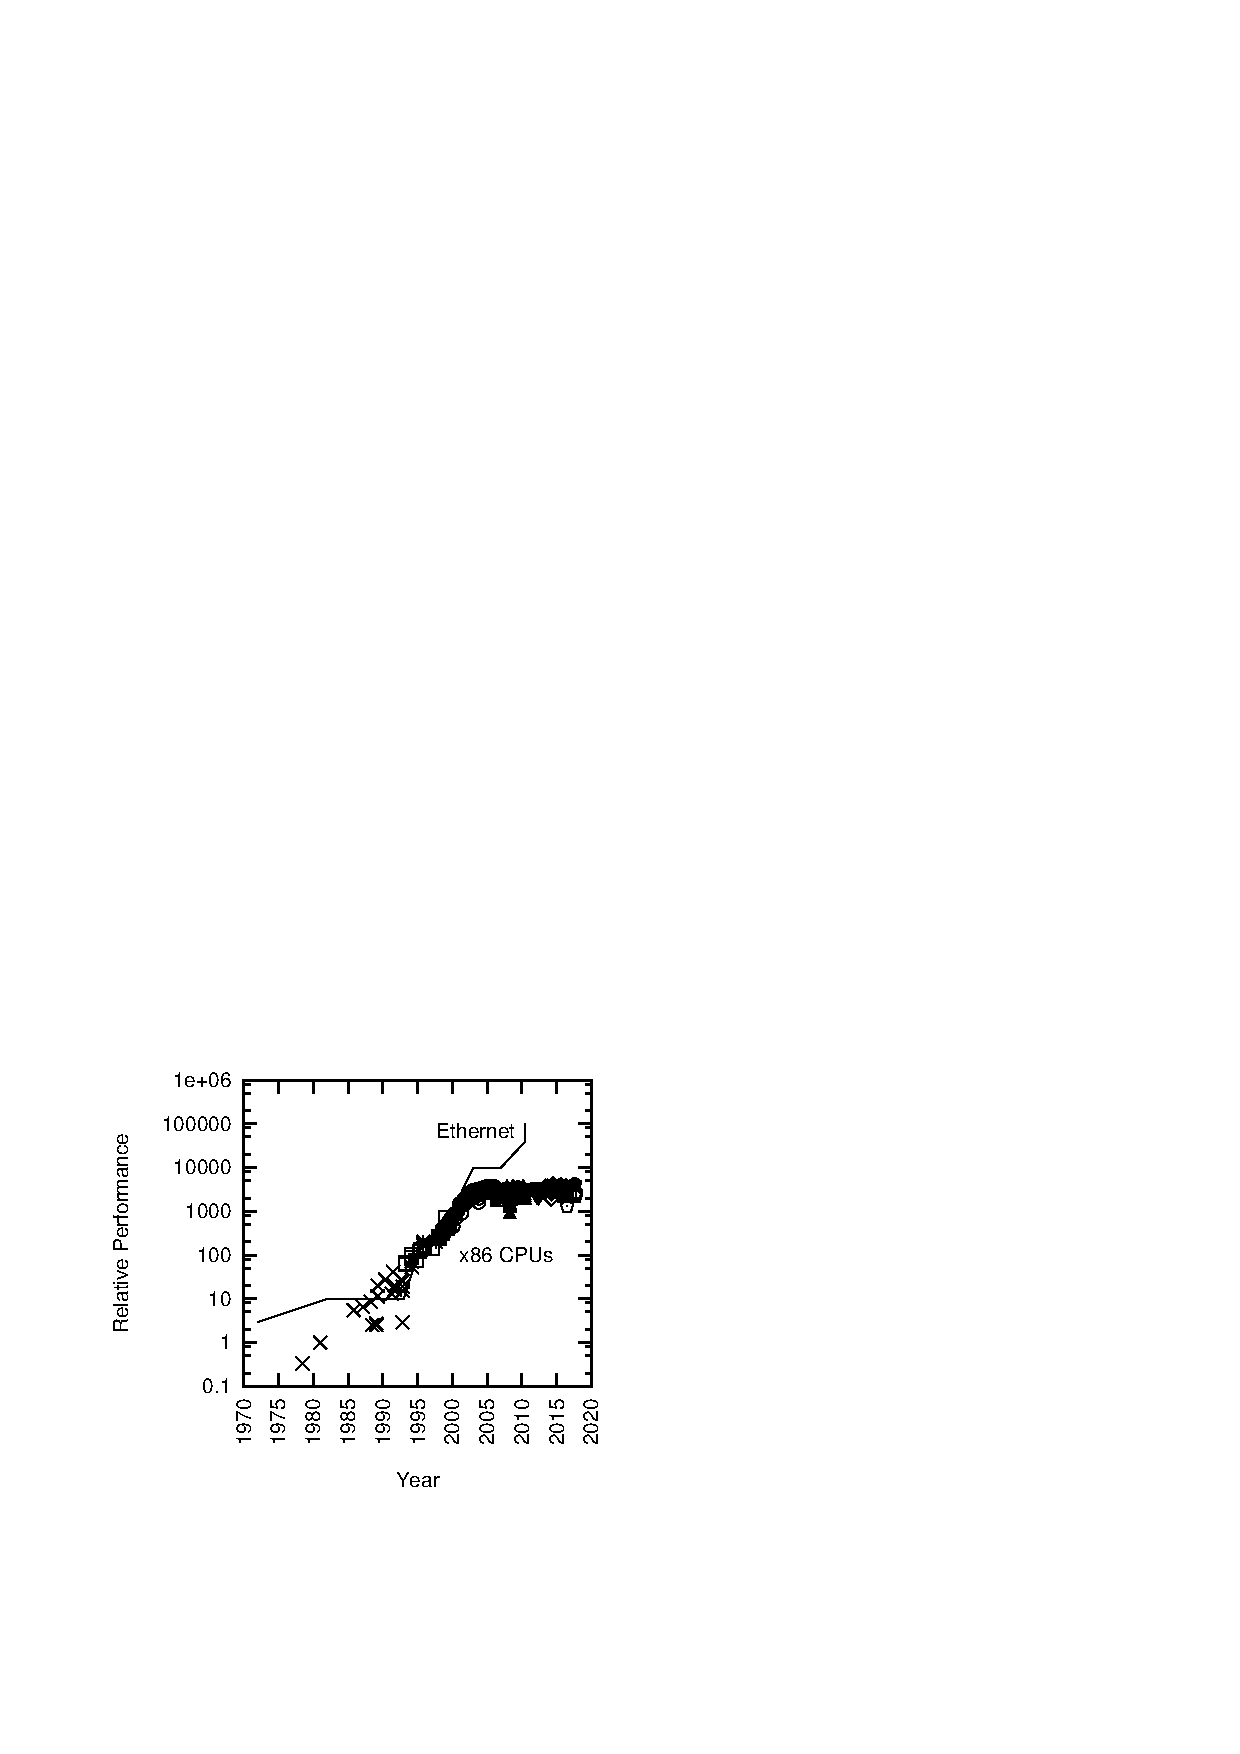
\includegraphics{SMPdesign/CPUvsEnet}}
\end{center}
\caption{Ethernet Bandwidth vs. Intel x86 CPU Performance}
\label{fig:SMPdesign:Ethernet Bandwidth vs. Intel x86 CPU Performance}
\end{figure}

이는 당신이 모든 프로그램을 멀티쓰레드 방식으로 코딩해야 한다는 의미가
\emph{아닙니다}.
다시 말하지만, 프로그램이 싱글 프로세서에서 충분히 빨리 동작한다면, SMP 동기화
기능들의 오버헤드와 복잡성으로부터 당신을 멀리 하십시오.
Figure~\ref{fig:SMPdesign:Sequential-Program Hash Table Search} 에 나와 있는
해시 테이블 탐색 코드의 단순성이 이 점을 강조합니다.\footnote{
이 섹션의 예들은 Hart 등~\cite{ThomasEHart2006a} 으로부터 얻어졌으며, 여러
	파일들로부터 관련된 코드를 모음으로써 켱쾌함을 위해 적용되었습니다.}
키 포인트는 병렬성으로 인한 속도향상은 CPU 들의 갯수에 제한된다는 것입니다.
반면, 예컨대 조심스럽게 선택된 데이터 구조와 같은 순차적 최적화를 통한
속도향상은 얼마든지 클 수 있습니다.
\iffalse

Please note that this does \emph{not} mean that you should code each
and every program in a multi-threaded manner.
Again, if a program runs quickly enough on a single processor,
spare yourself the overhead and complexity of SMP synchronization
primitives.
The simplicity of the hash-table lookup code in
Figure~\ref{fig:SMPdesign:Sequential-Program Hash Table Search}
underscores this point.\footnote{
	The examples in this section are taken from Hart et
	al.~\cite{ThomasEHart2006a}, adapted for clarity
	by gathering related code from multiple files.}
A key point is that speedups due to parallelism are normally
limited to the number of CPUs.
In contrast, speedups due to sequential optimizations, for example,
careful choice of data structure, can be arbitrarily large.
\fi

\begin{figure}[htbp]
{ \scriptsize
\begin{verbatim}
  1 struct hash_table
  2 {
  3   long nbuckets;
  4   struct node **buckets;
  5 };
  6
  7 typedef struct node {
  8   unsigned long key;
  9   struct node *next;
 10 } node_t;
 11
 12 int hash_search(struct hash_table *h, long key)
 13 {
 14   struct node *cur;
 15
 16   cur = h->buckets[key % h->nbuckets];
 17   while (cur != NULL) {
 18     if (cur->key >= key) {
 19       return (cur->key == key);
 20     }
 21     cur = cur->next;
 22   }
 23   return 0;
 24 }
\end{verbatim}
}
\caption{Sequential-Program Hash Table Search}
\label{fig:SMPdesign:Sequential-Program Hash Table Search}
\end{figure}

% ./test_hash_null.exe 1000 0/100 1 1024 1
% ./test_hash_null.exe: nmilli: 1000 update/total: 0/100 nelements: 1 nbuckets: 1024 nthreads: 1
% ./test_hash_null.exe: avg = 96.2913  max = 98.2337  min = 90.4095  std = 2.95314
% ./test_hash_null.exe: nmilli: 1000 update/total: 0/100 nelements: 1 nbuckets: 1024 nthreads: 1
% ./test_hash_null.exe: avg = 91.5592  max = 97.3315  min = 89.9885  std = 2.88925
% ./test_hash_null.exe: nmilli: 1000 update/total: 0/100 nelements: 1 nbuckets: 1024 nthreads: 1
% ./test_hash_null.exe: avg = 93.3568  max = 106.162  min = 89.8828  std = 6.40418

반면, 이런 행복한 상황에 처해 있는 게 아니라면, 계속 읽으세요!
\iffalse

On the other hand, if you are not in this happy situation, read on!
\fi

\subsection{Code Locking}
\label{sec:SMPdesign:Code Locking}

코드 락킹은 글로벌 락들만을 사용하기 때문에 상당히 간단합니다.\footnote{
	그게 아니라 데이터 구조체 안에 락들을 가지고 있거나, 자바의 경우,
	synchronized 인스턴스로 클래스들을 사용한다면,
	Section~\ref{sec:SMPdesign:Data Locking} 에 설명된 ``데이터 락킹'' 을
	사용하고 있는 겁니다.}
이 방법은 기존의 프로그램을 컬티 프로세서 위에서 동작하도록 하기 위해 코드
락킹을 사용하도록 수정하는 것은 특히 쉽습니다.
만약 프로그램이 하나의 공유자원만을 가지고 있다면, 코드 락킹은 최적의 성능을
제공할 것입니다.
하지만, 많은 거대하고 복잡한 프로그램들은 많은 수행이 크리티컬 섹션에서
일어나야만 할 것을 요구하고, 이는 곧 코드 락킹이 그 확장성을 크게 제한하게 하는
결과를 초래합니다.
\iffalse

Code locking is quite simple due to the fact that is uses only
global locks.\footnote{
	If your program instead has locks in data structures,
	or, in the case of Java, uses classes with synchronized
	instances, you are instead using ``data locking'', described
	in Section~\ref{sec:SMPdesign:Data Locking}.}
It is especially
easy to retrofit an existing program to use code locking in
order to run it on a multiprocessor.  If the program has
only a single shared resource, code locking will even give
optimal performance.
However, many of the larger and more complex programs
require much of the execution to
occur in critical sections, which in turn causes code locking
to sharply limits their scalability.
\fi

따라서, 전체 실행시간 중 작은 부분만을 크리티컬 섹션에서 수행하거나 작은
확장성만이 필요한 프로그램들에 대해서만 코드 락킹을 사용해야 합니다.
이런 경우, 코드 락킹은
Figure~\ref{fig:SMPdesign:Code-Locking Hash Table Search} 에서 볼 수 있듯,
순차적인 버전과 매우 유사하고 상대적으로 간단한 프로그램을 제공할 것입니다.
하지만, Figure~\ref{fig:SMPdesign:Sequential-Program Hash Table Search} 의
\co{hash_search()} 에서의 단순한 비교값 리턴은 이제 리턴 전에 락을 풀어야 하기
때문에 세개의 문장이 되었음을 알아 두시기 바랍니다.
\iffalse

Therefore, you should use code locking on programs that spend
only a small fraction of their execution time in critical sections or
from which only modest scaling is required.  In these cases,
code locking will provide a relatively simple program that is
very similar to its sequential counterpart,
as can be seen in
Figure~\ref{fig:SMPdesign:Code-Locking Hash Table Search}.
However, note that the simple return of the comparison in
\co{hash_search()} in
Figure~\ref{fig:SMPdesign:Sequential-Program Hash Table Search}
has now become three statements due to the need to release the
lock before returning.
\fi

\begin{figure}[htbp]
{ \scriptsize
\begin{verbatim}
  1 spinlock_t hash_lock;
  2
  3 struct hash_table
  4 {
  5   long nbuckets;
  6   struct node **buckets;
  7 };
  8
  9 typedef struct node {
 10   unsigned long key;
 11   struct node *next;
 12 } node_t;
 13
 14 int hash_search(struct hash_table *h, long key)
 15 {
 16   struct node *cur;
 17   int retval;
 18
 19   spin_lock(&hash_lock);
 20   cur = h->buckets[key % h->nbuckets];
 21   while (cur != NULL) {
 22     if (cur->key >= key) {
 23       retval = (cur->key == key);
 24       spin_unlock(&hash_lock);
 25       return retval;
 26     }
 27     cur = cur->next;
 28   }
 29   spin_unlock(&hash_lock);
 30   return 0;
 31 }
\end{verbatim}
}
\caption{Code-Locking Hash Table Search}
\label{fig:SMPdesign:Code-Locking Hash Table Search}
\end{figure}

안타깝게도, 코드 락킹은 여러 CPU 들이 락을 동시에 획득하려 하는, ``락 경쟁''
상황에 빠지기 쉬운 경향이 있습니다.
한 무리의 어린 아이들(또는 아이처럼 행동하는 어른들의 무리들) 을 보살펴야 하는
SMP 프로그래머들은 곧바로 Figure~\ref{fig:SMPdesign:Lock Contention} 에 그려진
것처럼 뭔가 단 하나를 사용하는 것의 위험성을 깨달을 것입니다.
\iffalse

Unfortunately, code locking is particularly prone to ``lock contention'',
where multiple CPUs need to acquire the lock concurrently.
SMP programmers who have taken care of groups of small children
(or groups of older people who are acting like children) will immediately
recognize the danger of having only one of something,
as illustrated in Figure~\ref{fig:SMPdesign:Lock Contention}.
\fi

% ./test_hash_codelock.exe 1000 0/100 1 1024 1
% ./test_hash_codelock.exe: nmilli: 1000 update/total: 0/100 nelements: 1 nbuckets: 1024 nthreads: 1
% ./test_hash_codelock.exe: avg = 164.115  max = 170.388  min = 161.659  std = 3.21857
% ./test_hash_codelock.exe: nmilli: 1000 update/total: 0/100 nelements: 1 nbuckets: 1024 nthreads: 1
% ./test_hash_codelock.exe: avg = 181.17  max = 198.4  min = 162.459  std = 15.8585
% ./test_hash_codelock.exe: nmilli: 1000 update/total: 0/100 nelements: 1 nbuckets: 1024 nthreads: 1
% ./test_hash_codelock.exe: avg = 167.651  max = 189.014  min = 162.144  std = 10.6819

% ./test_hash_codelock.exe 1000 0/100 1 1024 2
% ./test_hash_codelock.exe: nmilli: 1000 update/total: 0/100 nelements: 1 nbuckets: 1024 nthreads: 2
% ./test_hash_codelock.exe: avg = 378.481  max = 385.971  min = 374.235  std = 4.05934
% ./test_hash_codelock.exe: nmilli: 1000 update/total: 0/100 nelements: 1 nbuckets: 1024 nthreads: 2
% ./test_hash_codelock.exe: avg = 753.414  max = 1015.28  min = 377.734  std = 294.942
% ./test_hash_codelock.exe: nmilli: 1000 update/total: 0/100 nelements: 1 nbuckets: 1024 nthreads: 2
% ./test_hash_codelock.exe: avg = 502.737  max = 980.924  min = 374.406  std = 239.383

이 문제에 대한 해결책인 ``데이터 락킹'' 이 다음 섹션에 설명됩니다.
\iffalse

One solution to this problem, named ``data locking'', is described
in the next section.
\fi

\begin{figure}[htb]
\begin{center}
\resizebox{3in}{!}{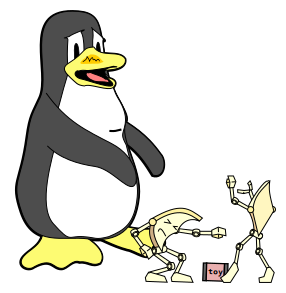
\includegraphics{cartoons/r-2014-Data-one-fighting}}
\end{center}
\caption{Lock Contention}
\ContributedBy{Figure}{fig:SMPdesign:Lock Contention}{Melissa Broussard}
\end{figure}

\subsection{Data Locking}
\label{sec:SMPdesign:Data Locking}

많은 데이터 구조체들이 각자 자기의 락을 갖는 조각들로 분할될 수 있습니다.
이렇게 되면 데이터 구조체의 각 조각들의 크리티컬 섹션들은 병렬적으로 실행될 수
있습니다, 각 조각의 크리티컬 섹션의 인스턴스는 한번에 하나씩만 수행될 수 있긴
하지만요.
경쟁상황이 줄어야만 하고, 동기화 오버헤드가 속도향상을 제한하지 않는 경우에는
데이터 락킹을 사용해야 합니다.
데이터 락킹은 여러 데이터 구조체 사이에 존재하는 너무 큰 크리티컬 섹션의
인스턴스들을 분산시킴으로써 경쟁상황을 줄여주는데, 예를 들어
Figure~\ref{fig:SMPdesign:Data-Locking Hash Table Search} 처럼 해시 테이블에서
해시 버킷 별로 크리티컬 섹션을 두는 식입니다.
향상된 확장성은 약간 추가적인 데이터 구조체인 \co{struct bucket} 의 형태로
복잡도를 약간 증가시킵니다.
\iffalse

Many data structures may be partitioned,
with each partition of the data structure having its own lock.
Then the critical sections for each part of the data structure
can execute in parallel,
although only one instance of the critical section for a given
part could be executing at a given time.
You should use data locking when contention must
be reduced, and where synchronization overhead is not
limiting speedups.
Data locking reduces contention by distributing the instances
of the overly-large critical section across multiple data structures,
for example, maintaining per-hash-bucket critical sections in a
hash table, as shown in
Figure~\ref{fig:SMPdesign:Data-Locking Hash Table Search}.
The increased scalability again results in a slight increase in complexity
in the form of an additional data structure, the \co{struct bucket}.
\fi

\begin{figure}[htbp]
{ \scriptsize
\begin{verbatim}
  1 struct hash_table
  2 {
  3   long nbuckets;
  4   struct bucket **buckets;
  5 };
  6
  7 struct bucket {
  8   spinlock_t bucket_lock;
  9   node_t *list_head;
 10 };
 11
 12 typedef struct node {
 13   unsigned long key;
 14   struct node *next;
 15 } node_t;
 16
 17 int hash_search(struct hash_table *h, long key)
 18 {
 19   struct bucket *bp;
 20   struct node *cur;
 21   int retval;
 22
 23   bp = h->buckets[key % h->nbuckets];
 24   spin_lock(&bp->bucket_lock);
 25   cur = bp->list_head;
 26   while (cur != NULL) {
 27     if (cur->key >= key) {
 28       retval = (cur->key == key);
 29       spin_unlock(&bp->bucket_lock);
 30       return retval;
 31     }
 32     cur = cur->next;
 33   }
 34   spin_unlock(&bp->bucket_lock);
 35   return 0;
 36 }
\end{verbatim}
}
\caption{Data-Locking Hash Table Search}
\label{fig:SMPdesign:Data-Locking Hash Table Search}
\end{figure}

Figure~\ref{fig:SMPdesign:Lock Contention} 에서 보였던 경쟁적인 상황과 달리,
데이터 락킹은 Figure~\ref{fig:SMPdesign:Data Locking} 에 그려진 것처럼 조화를
향상시킵니다 --- 그리고 병렬 프로그램에서, 이는 \emph{거의} 항상 향상된 성능과
확장성으로 이어집니다.
이런 이유로, 데이터 락킹은 DYNIX 와 DYNIX/ptx 운영체제의 Sequent 에서 매우 많이
사용되었습니다~\cite{Beck85,Inman85,Garg90,Dove90,McKenney92b,McKenney92a,McKenney93}.
\iffalse

In contrast with the contentious situation
shown in Figure~\ref{fig:SMPdesign:Lock Contention},
data locking helps promote harmony, as illustrated by
Figure~\ref{fig:SMPdesign:Data Locking} --- and in parallel programs,
this \emph{almost} always translates into increased performance and
scalability.
For this reason, data locking was heavily used by Sequent in
both its DYNIX and DYNIX/ptx operating
systems~\cite{Beck85,Inman85,Garg90,Dove90,McKenney92b,McKenney92a,McKenney93}.
\fi

\begin{figure}[htb]
\begin{center}
\resizebox{3in}{!}{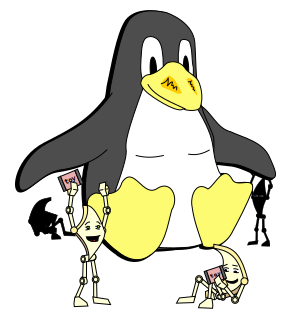
\includegraphics{cartoons/r-2014-Data-many-happy}}
\end{center}
\caption{Data Locking}
\ContributedBy{Figure}{fig:SMPdesign:Data Locking}{Melissa Broussard}
\end{figure}

% ./test_hash_spinlock.exe 1000 0/100 1 1024 1
% ./test_hash_spinlock.exe: nmilli: 1000 update/total: 0/100 nelements: 1 nbuckets: 1024 nthreads: 1
% ./test_hash_spinlock.exe: avg = 158.118  max = 162.404  min = 156.199  std = 2.19391
% ./test_hash_spinlock.exe: nmilli: 1000 update/total: 0/100 nelements: 1 nbuckets: 1024 nthreads: 1
% ./test_hash_spinlock.exe: avg = 157.717  max = 162.446  min = 156.415  std = 2.36662
% ./test_hash_spinlock.exe: nmilli: 1000 update/total: 0/100 nelements: 1 nbuckets: 1024 nthreads: 1
% ./test_hash_spinlock.exe: avg = 158.369  max = 164.75  min = 156.501  std = 3.19454

% ./test_hash_spinlock.exe 1000 0/100 1 1024 2
% ./test_hash_spinlock.exe: nmilli: 1000 update/total: 0/100 nelements: 1 nbuckets: 1024 nthreads: 2
% ./test_hash_spinlock.exe: avg = 223.426  max = 422.948  min = 167.858  std = 100.136
% ./test_hash_spinlock.exe: nmilli: 1000 update/total: 0/100 nelements: 1 nbuckets: 1024 nthreads: 2
% ./test_hash_spinlock.exe: avg = 235.462  max = 507.134  min = 167.466  std = 135.836
% ./test_hash_spinlock.exe: nmilli: 1000 update/total: 0/100 nelements: 1 nbuckets: 1024 nthreads: 2
% ./test_hash_spinlock.exe: avg = 305.807  max = 481.685  min = 167.939  std = 132.589

하지만, 어린 아이들을 돌봐 본 사람이라면 증명할 수 있듯이, 충분히 가서 놀 수
있는 공간을 주는 것이 평안을 보장하지는 않습니다.
예를 들어, 리눅스 커널은 파일과 디렉토리들의 캐시 (``dcache'' 라 불립니다) 를
갖습니다.
이 캐시의 각 원소들은 자신의 락을 갖습니다만, 루트 디렉토리에 해당하는 원소들과
그것의 직접적인 자식들은 다른 원소들에 비해 훨씬 많이 순회됩니다.
이는 많은 CPU 들이 이 자주 접근되는 원소들의 락에 경쟁을 하게 되는 결과를
초래해서, Figure~\ref{fig:SMPdesign:Data and Skew} 에 보여진 것과 같은 상황을
초래하고 맙니다.
\iffalse

However, as those who have taken care of small children can again attest,
even providing enough to go around is no guarantee of tranquillity.
The analogous situation can arise in SMP programs.
For example, the Linux kernel maintains a cache of files and directories
(called ``dcache'').
Each entry in this cache has its own lock, but the entries corresponding
to the root directory and its direct descendants are much more likely to
be traversed than are more obscure entries.
This can result in many CPUs contending for the locks of these popular
entries, resulting in a situation not unlike that
shown in Figure~\ref{fig:SMPdesign:Data and Skew}.
\fi

\begin{figure}[htb]
\begin{center}
\resizebox{3in}{!}{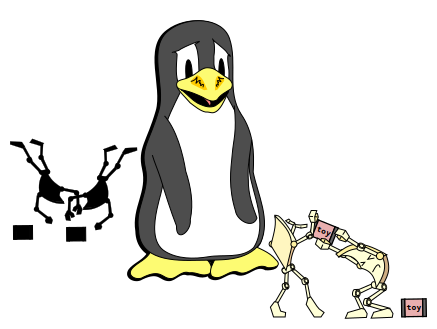
\includegraphics{cartoons/r-2014-Data-many-fighting}}
\end{center}
\caption{Data Locking and Skew}
\ContributedBy{Figure}{fig:SMPdesign:Data and Skew}{Melissa Broussard}
\end{figure}

많은 경우, 알고리즘들은 데이터 스큐를 줄이도록 설계될 수 있고, 어떤 경우에는
아예 그것들을 없애버릴 수도 있습니다 (리눅스 커널의 dcache 에서도 가능한 것으로
나타난 것처럼요~\cite{McKenney04a}).
데이터 락킹은 종종 해시 테이블처럼 분할될 수 있는 데이터 구조체에 사용됩니다만,
여러 존재가 각각 어떤 데이터 구조체의 인스턴스로 표현될 수 있는 경우에도
사용됩니다.
리눅스 커널 2.6.17 버전의 태스크 리스트는 후자의 한 예로, 각 태스크 구조체는
자신의 \co{proc_lock} 을 갖습니다.

다이나믹하게 할당되는 구조체들에서의 데이터 락킹의 핵심 문제는 해당 구조체가
해당 락이 잡혀있는 동안은 존재하는 상태를 유지해야 한다는 것입니다.
Figure~\ref{fig:SMPdesign:Data-Locking Hash Table Search} 의 코드는 이 문제를
락들을 정적으로 할당된 해시 버킷들에 넣어두고, 절대 메모리에서 해제시키지 않는
것으로 해결합니다.
하지만, 이 트릭은 해시 테이블의 크기가 바뀔 수 있다면 락들이 다이나믹하게
할당되어야 하므로 제대로 동작하지 않을 것입니다.
이 경우, 해시 버킷들을 그 락들이 잡혀있는 동안은 메모리 해제되지 않도록 하는
어떤 수단이 필요할 것입니다.
\iffalse

In many cases, algorithms can be designed to reduce the instance of
data skew, and in some cases eliminate it entirely
(as appears to be possible with the Linux kernel's dcache~\cite{McKenney04a}).
Data locking is often used for partitionable data structures such as
hash tables, as well as in situations where multiple entities are each
represented by an instance of a given data structure.
The task list in version 2.6.17 of the Linux kernel is an example of the
latter, each task structure having its own \co{proc_lock}.

A key challenge with data locking on dynamically allocated structures
is ensuring that the structure remains in existence while the lock is
being acquired.
The code in
Figure~\ref{fig:SMPdesign:Data-Locking Hash Table Search}
finesses this challenge by placing the locks in the statically allocated
hash buckets, which are never freed.
However, this trick would not work if the hash table were resizeable,
so that the locks were now dynamically allocated.
In this case, there would need to be some means to prevent the hash
bucket from being freed during the time that its lock was being acquired.
\fi

\QuickQuiz{}
	구조체가 그것의 락이 잡혀 있는 동안은 메모리 해제 되지 않도록 할 수
	있는 방법들은 어떤 것들이 있을까요?
	\iffalse

	What are some ways of preventing a structure from being freed while
	its lock is being acquired?
	\fi
\QuickQuizAnswer{
	여기 \emph{존재 보장} 문제를 위한 해결책 몇가지가 있습니다:
	\iffalse

	Here are a few possible solutions to this \emph{existence guarantee}
	problem:
	\fi

	\begin{enumerate}
	\item	구조체별 락이 잡혀 있는 동안 잡혀 있는 정적으로 할당된 락을
		두는 것으로, 계층적 락킹의 한 예입니다
		(Section~\ref{sec:SMPdesign:Hierarchical Locking} 을
		참고하세요).
		물론, 이런 목적으로 하나의 글로벌 락을 사용하는 것은
		허용불가능할 정도로 높은 락 경쟁 상황을 가져와서 극적인 성능과
		확장성의 하락을 가져올 수 있습니다.
	\item	정적으로 할당된 락들의 배열을 두어서, 구조체의 어드레스를
		해싱해서 잡아야 할 락을 고르는 것으로,
		Chapter~\ref{chp:Locking} 에서 설명된 방식입니다.
		주어진 해시 함수가 충분히 높은 성능을 갖는다면, 이는 하나의
		글로벌 락이 갖는 확장성의 한계를 해결할 수 있습니다만, 읽기가
		대부분인 상황에서는 락 획득 오버헤드가 수용불가할 정도로 성능을
		떨어뜨릴 수 있습니다.
	\item	가비지 콜렉터를 제공하는 소프트웨어 환경이라면 가비지 콜렉터를
		사용해서, 구조체가 참조되어 있는 동안은 메모리 해제되지 않도록
		하는 것입니다.
		이 방법은 잘 동작하고, 존재-보장의 짐을 (그리고 그외의 것들을)
		개발자의 어깨에서 내려놓게 하지만, 프로그램의 가비지 콜렉션의
		오버헤드를 갖습니다.
		가비지 콜렉션 기술은 지난 수십년간 상당히 진보했지만, 그
		오버헤드는 일부 어플리케이션에서는 수용하기 어려울 만큼 높을 수
		있습니다.
		또한, 일부 어플리케이션들은 개발자가 데이터 구조체의 배치와
		위치의 조정에 대해 대부분의 가비지 콜렉션 환경에 비해 많은
		연습을 필요로 할수도 있습니다.
	\iffalse

	\item	Provide a statically allocated lock that is held while
		the per-structure lock is being acquired, which is an
		example of hierarchical locking (see
		Section~\ref{sec:SMPdesign:Hierarchical Locking}).
		Of course, using a single global lock for this purpose
		can result in unacceptably high levels of lock contention,
		dramatically reducing performance and scalability.
	\item	Provide an array of statically allocated locks, hashing
		the structure's address to select the lock to be acquired,
		as described in Chapter~\ref{chp:Locking}.
		Given a hash function of sufficiently high quality, this
		avoids the scalability limitations of the single global
		lock, but in read-mostly situations, the lock-acquisition
		overhead can result in unacceptably degraded performance.
	\item	Use a garbage collector, in software environments providing
		them, so that a structure cannot be deallocated while being
		referenced.
		This works very well, removing the existence-guarantee
		burden (and much else besides) from the developer's
		shoulders, but imposes the overhead of garbage collection
		on the program.
		Although garbage-collection technology has advanced
		considerably in the past few decades, its overhead
		may be unacceptably high for some applications.
		In addition, some applications require that the developer
		exercise more control over the layout and placement of
		data structures than is permitted by most garbage collected
		environments.
	\fi
	\item	가비지 콜렉터의 특수한 경우로, 글로벌 레퍼런스 카운터를 두거나
		레퍼런스 카운터들의 글로벌한 배열을 두는 방법이 있습니다.
	\item	안에서-밖으로의 참조 카운트라 생각할 수 있는, \emph{해저드
		포인터}~\cite{MagedMichael04a} 들을 사용하는 방법이 있습니다.
		해저드 포인터 기반의 알고리즘들은 쓰레드별 포인터들의 리스트를
		두어서, 이 리스트들에 있는 포인터의 존재가 연관된 구조체로의
		참조처럼 동작하게 합니다.
		해저드 포인터들은 흥미로운 연구 방향입니다만, 상품화 단계
		(2008년도 시점에선) 에선 아직 잘 쓰여지지 않고 있습니다.
	\item	트랜잭셔널
		메모리(TM)~\cite{Herlihy93a,DBLomet1977SIGSOFT,Shavit95} 를
		사용해서 데이터 구조체로 요청되는 각각의 참조와 수정이
		어토믹하게 수행되도록 하는 방법이 있습니다.
		TM 은 최근의 수년간 대단한 흥분을 일으켰고 상품 단계
		소프트웨어에서 일부 사용될 것처럼 보였지만, 개발자들은 몇가지
		주의를 기울여야
		하며~\cite{Blundell2005DebunkTM,Blundell2006TMdeadlock,McKenney2007PLOSTM}
		이는 특히 성능에 영향을 주는 코드에선 더더욱 그렇습니다.
		특히, 존재 보장은 트랜잭션이 글로벌 레퍼런스부터 업데이트되는
		데이터 원소들에 이르기까지 전체를 감싸야 할 것을 필요로 합니다.
	\item	극단적으로 가벼운 가비지 콜렉터의 추상화로 생각될 수 있는, RCU
		를 사용하는 것입니다.
		업데이트를 하는 쪽은 RCU 로 보호되는 데이터 구조체를 RCU
		읽는쪽이 여전히 참조를 하고 있는 동안은 메모리에서 해제시킬 수
		없습니다.
		RCU 는 읽기가 대부분인 데이터 구조체에서 상당히 많이 사용되고
		있고, Chapter~\ref{chp:Deferred Processing} 에서 이야기될
		것입니다.
	\iffalse

	\item	As a special case of a garbage collector, use a global
		reference counter, or a global array of reference counters.
	\item	Use \emph{hazard pointers}~\cite{MagedMichael04a}, which
		can be thought of as an inside-out reference count.
		Hazard-pointer-based algorithms maintain a per-thread list of
		pointers, so that the appearance of a given pointer on
		any of these lists acts as a reference to the corresponding
		structure.
		Hazard pointers are an interesting research direction, but
		have not yet seen much use in production (written in 2008).
	\item	Use transactional memory
		(TM)~\cite{Herlihy93a,DBLomet1977SIGSOFT,Shavit95},
		so that each reference and
		modification to the data structure in question is
		performed atomically.
		Although TM has engendered much excitement in recent years,
		and seems likely to be of some use in production software,
		developers should exercise some
		caution~\cite{Blundell2005DebunkTM,Blundell2006TMdeadlock,McKenney2007PLOSTM},
		particularly in performance-critical code.
		In particular, existence guarantees require that the
		transaction cover the full path from a global reference
		to the data elements being updated.
	\item	Use RCU, which can be thought of as an extremely lightweight
		approximation to a garbage collector.
		Updaters are not permitted to free RCU-protected
		data structures that RCU readers might still be referencing.
		RCU is most heavily used for read-mostly data structures,
		and is discussed at length in
		Chapter~\ref{chp:Deferred Processing}.
	\fi
	\end{enumerate}

	존재 보장에 대해 더 많은 내용을 위해선 Chapter~\ref{chp:Locking} 과
	\ref{chp:Deferred Processing} 을 참고하세요.
	\iffalse

	For more on providing existence guarantees, see
	Chapters~\ref{chp:Locking} and \ref{chp:Deferred Processing}.
	\fi
} \QuickQuizEnd

\subsection{Data Ownership}
\label{sec:SMPdesign:Data Ownership}

데이터 소유권은 주어진 데이터 구조체를 쓰레드들이나 CPU 들로 쪼개서, 각
쓰레드/CPU 는 데이터의 자신에게 할당된 부분집합을 어떤 동기화 오버헤드 없이
접근할 수 있습니다.
하지만, 어떤 쓰레드가 다른 쓰레드의 데이터에 접근하길 원한다면, 이는 곧바로 될
수는 없습니다.
대신, 이 쓰레드는 다른 쓰레드와 먼저 통신을 해서 다른 쓰레드가 그 일을 대신
해주거나, 또는 그 데이터의 소유권을 이전해 주도록 해야 합니다.

데이터 소유권은 불가사의해 보일 수 있지만, 매우 자주 사용됩니다:
\iffalse

Data ownership partitions a given data structure over the threads
or CPUs, so that each thread/CPU accesses its subset of the data
structure without any synchronization overhead whatsoever.
However, if one thread wishes to access some other thread's data,
the first thread is unable to do so directly.
Instead, the first thread must communicate with the second thread,
so that the second thread performs the operation on behalf of the
first, or, alternatively, migrates the data to the first thread.

Data ownership might seem arcane, but it is used very frequently:
\fi
\begin{enumerate}
\item	한 CPU 나 쓰레드에 의해서만 접근될 수 있는 변수 (C 와 C++ 에서의 {\tt
	auto} 변수와 같은) 들은 모두 해당 CPU 나 프로세스에게 소유되어
	있습니다.
\item	사용자 인터페이스의 한 인스턴스는 해당 사용자의 컨텍스트를 소유합니다.
	병렬 데이터베이스 엔진과 상호작용하는 어플리케이션들은 그것들이 순차적
	프로그램인 것마냥 작성되는 것이 매우 흔한 일입니다.
	그런 어플리케이션들은 사용자 인터페이스와 그/그녀의 현재 동작을
	소유합니다.
	명시적인 병렬성은 따라서 데이터베이스 엔진 그 자체에 국한되어 있습니다.
\item	파라미터를 사용하는 시뮬레이션들은 종종 각 쓰레드가 파라미터 공간의
	특정 영역에 소유권을 갖게 하는 방법으로 병렬화 되곤 합니다.
	이런 타입의 문제를 위한 컴퓨팅 프레임웍도 존재합니다~\cite{BOINC2008}.
\iffalse

\item	Any variables accessible by only one CPU or thread
	(such as {\tt auto} variables in C
	and C++) are owned by that CPU or process.
\item	An instance of a user interface owns the corresponding
	user's context.  It is very common for applications
	interacting with parallel database engines to be
	written as if they were entirely sequential programs.
	Such applications own the user interface and his current
	action.  Explicit parallelism is thus confined to the
	database engine itself.
\item	Parametric simulations are often trivially parallelized
	by granting each thread ownership of a particular region
	of the parameter space.
	There are also computing frameworks designed for this
	type of problem~\cite{BOINC2008}.
\fi
\end{enumerate}

상당히 많은 공유가 존재한다면, 이 쓰레드들이나 CPU 들 사이의 통신은 상당한
복잡도와 오버헤드를 만들어낼 것입니다.
더 나아가서, 가장 많이 사용되는 데이터가 단일 CPU 에게 소유되어 있게 된다면, 이
CPU 는 ``핫스팟'' 이 될 것이고, Figure~\ref{fig:SMPdesign:Data and Skew} 에
그려진 것과 같은 결과를 낼 것입니다.
하지만, 공유가 필요하지 않은 상황이라면,
Figure~\ref{fig:SMPdesign:Sequential-Program Hash Table Search} 에 보여진
것처럼 데이터 소유권은 이상적인 성능을 내고, 순차적 프로그램처럼 간단해질 수
있을 것입니다.
그런 상황은 종종 ``당황스러울 정도로 병렬적'' 이라 불리곤 하고,
Figure~\ref{fig:SMPdesign:Data Locking} 에서 앞서 본것과 같은 상황과 닮아
있습니다.
\iffalse

If there is significant sharing, communication between the threads
or CPUs can result in significant complexity and overhead.
Furthermore, if the most-heavily used data happens to be that owned
by a single CPU, that CPU will be a ``hot spot'', sometimes with
results resembling that shown in Figure~\ref{fig:SMPdesign:Data and Skew}.
However, in situations where no sharing is required, data ownership
achieves ideal performance, and with code that can be as simple
as the sequential-program case shown in
Figure~\ref{fig:SMPdesign:Sequential-Program Hash Table Search}.
Such situations are often referred to as ``embarrassingly
parallel'', and, in the best case, resemble the situation
previously shown in Figure~\ref{fig:SMPdesign:Data Locking}.
\fi

% ./test_hash_null.exe 1000 0/100 1 1024 1
% ./test_hash_null.exe: nmilli: 1000 update/total: 0/100 nelements: 1 nbuckets: 1024 nthreads: 1
% ./test_hash_null.exe: avg = 96.2913  max = 98.2337  min = 90.4095  std = 2.95314
% ./test_hash_null.exe: nmilli: 1000 update/total: 0/100 nelements: 1 nbuckets: 1024 nthreads: 1
% ./test_hash_null.exe: avg = 91.5592  max = 97.3315  min = 89.9885  std = 2.88925
% ./test_hash_null.exe: nmilli: 1000 update/total: 0/100 nelements: 1 nbuckets: 1024 nthreads: 1
% ./test_hash_null.exe: avg = 93.3568  max = 106.162  min = 89.8828  std = 6.40418

% ./test_hash_null.exe 1000 0/100 1 1024 2
% ./test_hash_null.exe: nmilli: 1000 update/total: 0/100 nelements: 1 nbuckets: 1024 nthreads: 2
% ./test_hash_null.exe: avg = 45.4526  max = 46.4281  min = 45.1954  std = 0.487791
% ./test_hash_null.exe: nmilli: 1000 update/total: 0/100 nelements: 1 nbuckets: 1024 nthreads: 2
% ./test_hash_null.exe: avg = 46.0238  max = 49.2861  min = 45.1852  std = 1.63127
% ./test_hash_null.exe: nmilli: 1000 update/total: 0/100 nelements: 1 nbuckets: 1024 nthreads: 2
% ./test_hash_null.exe: avg = 46.6858  max = 52.6278  min = 45.1761  std = 2.97102

또다른 중요한 데이터 소유권 상황은 데이터가 읽기 전용인 경우, 모든 쓰레드가
복사본을 통해 그것을 ``소유'' 할 수 있는 경우입니다.

데이터 소유권은 Chapter~\ref{chp:Data Ownership} 에서 좀 더 자세히 다뤄질
겁니다.
\iffalse

Another important instance of data ownership occurs when the data
is read-only, in which case,
all threads can ``own'' it via replication.

Data ownership will be presented in more detail in
Chapter~\ref{chp:Data Ownership}.
\fi

\subsection{Locking Granularity and Performance}
\label{sec:SMPdesign:Locking Granularity and Performance}

이 섹션은 락킹 빈도와 성능 사이의 관계를 수학적인 동기화 효율성 관점에서
살펴봅니다.
수학이 지루한 독자분들은 이 섹션을 건너뛰셔도 됩니다.

사용할 방법은 하나의 공유되는 글로벌 변수에 대해 동작하는 동기화 메커니즘의
효율성을 위한 간단한 큐잉 모델을 M/M/1 큐를 기반으로 사용해 보는 것입니다.
M/M/1 큐잉 모델들은 지수적으로 분포되는 ``도착간 비율 (inter-arrival rate)''
$\lambda$ 와 지수적으로 분포되는 ``서비스 비율 (service rate)'' $\mu$ 에
기반합니다.
도착간 비율 $\lambda$ 는 만약 동기화 비용이 전혀 들지 않는다면 시스템이 처리할
수 있는, 초당 동기화 오퍼레이션들의 평균 숫자로 생각될 수 있는데, 달리 말하자면
$\lambda$ 는 작업의 비동기 유닛의 오버헤드의 역수입니다.
예를 들어, 일의 각 유닛이 트랜잭션이고, 각 트랜잭션이 처리되는데 동기화
오버헤드를 제외하고 1 밀리세컨드가 걸린다면, $\lambda$ 는 초당 1,000 트랜잭션이
될 것입니다.
\iffalse

This section looks at locking granularity and performance from
a mathematical synchronization-efficiency viewpoint.
Readers who are uninspired by mathematics might choose to skip
this section.

The approach is to use a crude queueing model for the efficiency of
synchronization mechanism that operate on a single shared global
variable, based on an M/M/1 queue.
M/M/1 queuing models are based on an exponentially distributed
``inter-arrival rate'' $\lambda$ and an exponentially distributed
``service rate'' $\mu$.
The inter-arrival rate $\lambda$ can be thought of as the average
number of synchronization operations per second that the system
would process if the synchronization were free, in other words,
$\lambda$ is an inverse measure of the overhead of each non-synchronization
unit of work.
For example, if each unit of work was a transaction, and if each transaction
took one millisecond to process, excluding synchronization overhead,
then $\lambda$ would be 1,000 transactions per second.
\fi

서비스 비율 $\mu$ 는 비슷하게 정의됩니다만, CPU 들이 각자의 동기화
오퍼레이션들을 완료하기를 기다려야 한다는 사실을 무시하고 각 트랜잭션의
오버헤드가 존재하지 않는다면 시스템이 1초 안에 처리할 수 있는 동기화
오퍼레이션들의 수의 평균으로, 달리 말하자면, $\mu$ 는 컨텐션이 없을 때의 동기화
오버헤드라고 생각될 수 있겠습니다.
예를 들어, 각 동기화 오퍼레이션이 어토믹 값 증가 인스트럭션을 내포하고 있고,
컴퓨터 시스템은 각 CPU 에서 각자의 변수에 25 나노세컨드마다 어토믹 값 증가
인스트럭션을 수행할 수 있다고 해 봅시다.\footnote{
	물론, 같은 공유 변수의 값을 증가시키는 8 개의 CPU 가 존재한다면, 각각의
	CPU 는 자신의 값 증가 작업을 위해 25 나노세컨드를 소모하기 전에 다른
	CPU 들이 각자의 값 증가 작업을 마무리 할 때까지 175 나노세컨드를
	기다려야 할 것입니다.
	실제로는, 이 대기는 더 길어질텐데 그 변수를 한 CPU 에서 다른 CPU 로
	옮기는 시간도 걸리기 때문입니다.}
따라서 $\mu$ 의 값은 초당 40,000,000 어토믹 값 증가 일 것입니다.

물론, $\lambda$ 의 값은 CPU 수가 늘어나면 함께 늘어날텐데, 각 CPU 가 독립적으로
트랜잭션들을 처리할 수 있기 때문입니다 (다시 말하지만, 동기화를 무시합니다):

\iffalse

The service rate $\mu$ is defined similarly, but for the average
number of synchronization operations per second that the system
would process if the overhead of each transaction was zero, and
ignoring the fact that CPUs must wait on each other to complete
their synchronization operations, in other words, $\mu$ can be roughly
thought of as the synchronization overhead in absence of contention.
For example, suppose that each synchronization operation involves an atomic
increment instruction, and that a computer system is able to do
an atomic increment every 25 nanoseconds on each CPU
to a private variable.\footnote{
	Of course, if there are 8 CPUs all incrementing the same
	shared variable, then each CPU must wait at least 175 nanoseconds
	for each of the other CPUs to do its increment before consuming
	an additional 25 nanoseconds doing its own increment.
	In actual fact, the wait will be longer due to the need
	to move the variable from one CPU to another.}
The value of $\mu$ is therefore about 40,000,000 atomic increments
per second.

Of course, the value of $\lambda$ increases with increasing numbers of
CPUs, as each CPU is capable of processing transactions independently
(again, ignoring synchronization):
\fi

\begin{equation}
	\lambda = n \lambda_0
\end{equation}

$n$ 은 CPU 들의 갯수이고 $\lambda_0$ 는 단일 CPU 의 트랜잭션 처리 가능량입니다.
단일 CPU 가 하나의 트랜잭션을 처리하는데 걸릴 것으로 기대되는 시간은
$1 / \lambda_0$ 임을 기억해 두십시오.

이 CPU 들은 다른 CPU 들이 각각 하나의 공유 변수의 값을 증가시킬 동안
``줄을 서서 기다려야'' 하기 때문에, 기대되는 전체 대기 시간을 표현하는데 M/M/1
큐잉 모델을 다음과 같이 사용할 수 있습니다:
\iffalse

where $n$ is the number of CPUs and $\lambda_0$ is the transaction-processing
capability of a single CPU.
Note that the expected time for a single CPU to execute a single transaction
is $1 / \lambda_0$.

Because the CPUs have to ``wait in line'' behind each other to get their
chance to increment the single shared variable, we can use the M/M/1
queueing-model expression for the expected total waiting time:
\fi

\begin{equation}
	T = \frac{1}{\mu - \lambda}
\end{equation}

앞의 $\lambda$ 값을 대입하면:
\iffalse

Substituting the above value of $\lambda$:
\fi

\begin{equation}
	T = \frac{1}{\mu - n \lambda_0}
\end{equation}

이제, 효율성은 동기화 없을 때 트랜잭션 하나를 처리하는데 필요한 시간 ($1 /
\lambda_0$) 과 동기화를 포함해서 필요한 시간 ($T + 1 / \lambda_0$) 사이의
비율입니다:
\iffalse

Now, the efficiency is just the ratio of the time required to process
a transaction in absence of synchronization ($1 / \lambda_0$)
to the time required including synchronization ($T + 1 / \lambda_0$):
\fi

\begin{equation}
	e = \frac{1 / \lambda_0}{T + 1 / \lambda_0}
\end{equation}

앞의 $T$ 값을 대입하고 간략화 하면:
\iffalse

Substituting the above value for $T$ and simplifying:
\fi

\begin{equation}
	e = \frac{\frac{\mu}{\lambda_0} - n}{\frac{\mu}{\lambda_0} - (n - 1)}
\end{equation}

하지만 $\mu / \lambda_0$ 의 값은 그저 트랜잭션을 처리하는데 필요한 시간과
(경쟁상황이 없는 상태에서의) 동기화 자체 오버헤드 간의 비율입니다.
이 비율을 $f$ 라고 하면, 이렇게 됩니다:
\iffalse

But the value of $\mu / \lambda_0$ is just the ratio of the time required
to process the transaction (absent synchronization overhead) to that of 
the synchronization overhead itself (absent contention).
If we call this ratio $f$, we have:
\fi

\begin{equation}
	e = \frac{f - n}{f - (n - 1)}
\end{equation}

\begin{figure}[tbp]
\begin{center}
\resizebox{3in}{!}{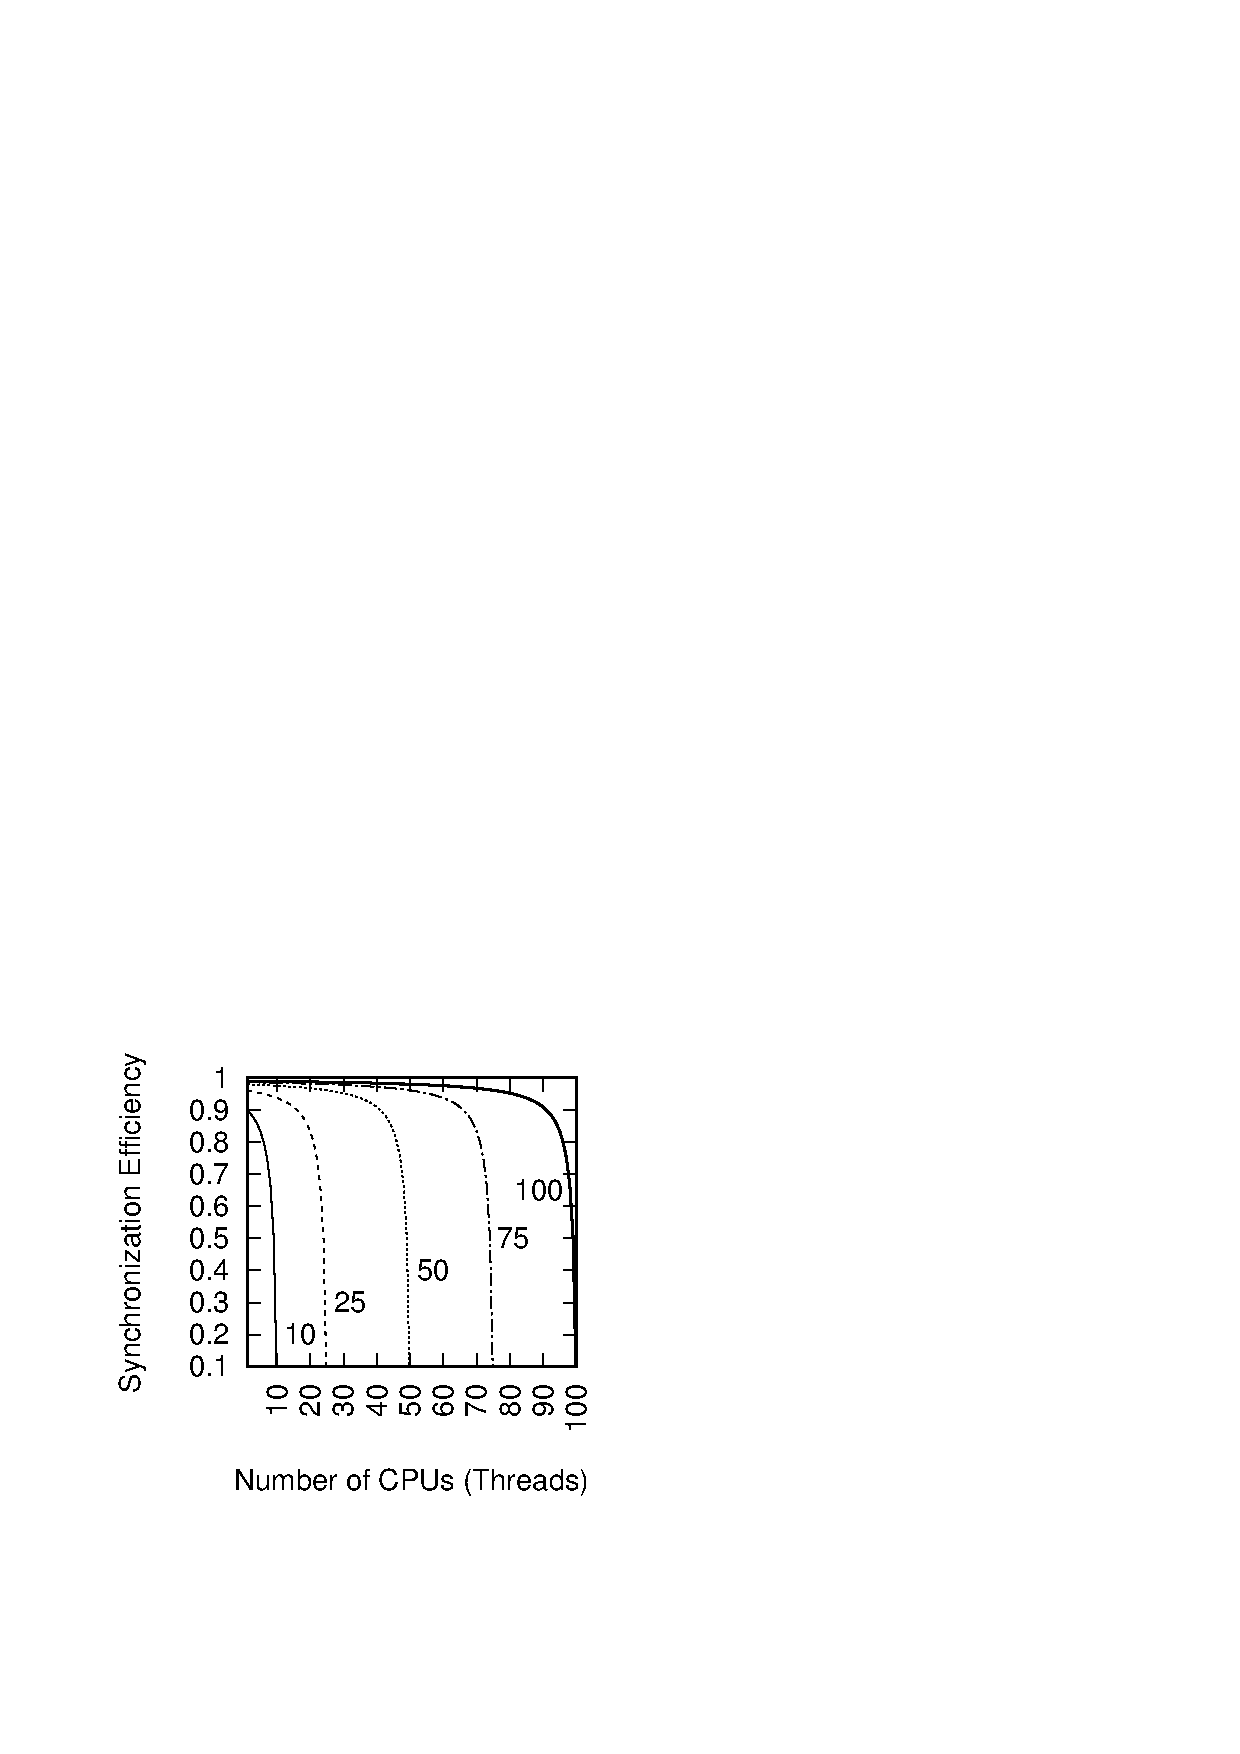
\includegraphics{SMPdesign/synceff}}
\end{center}
\caption{Synchronization Efficiency}
\label{fig:SMPdesign:Synchronization Efficiency}
\end{figure}

Figure~\ref{fig:SMPdesign:Synchronization Efficiency} 는 동기화 효율성 $e$ 가
CPU/쓰레드 수 $n$ 에 의해 변화되는 모습을 오버헤드 비율 $f$ 몇개의 값과 함께
보여줍니다.
예를 들어, 25 나노세컨드 걸리는 어토믹 값 증가 연산을 사용하면 $f=10$ 선은 각
CPU 가 매 250 나노세컨드마다 어토믹 값 증가 연산을 시도하고, $f=100$ 라인은 각
CPU 가 수천개의 인스트럭션이 처리될 수 있는 시간인 2.5 마이크로세컨드마다
어토믹 값 증가 연산을 시도합니다.
각 조합의 결과가 CPU 나 쓰레드의 수가 늘어남에 따라 급격하게 떨어지는 것으로
보아, 하나의 글로벌 공유 변수에의 어토믹 조정을 통한 동기화 메커니즘은 현재의
하드웨어에서 많이 사용되면 잘 확장되지 못할 것이라 결론 내릴 수 있습니다.
이건 이 규칙들을 수학적으로 그려본 것으로, Chapter~\ref{chp:Counting} 에서
이야기한 병렬 카운팅 알고리즘을 이끌어내게 합니다.
\iffalse

Figure~\ref{fig:SMPdesign:Synchronization Efficiency} plots the synchronization
efficiency $e$ as a function of the number of CPUs/threads $n$ for
a few values of the overhead ratio $f$.
For example, again using the 25-nanosecond atomic increment, the
$f=10$ line corresponds to each CPU attempting an atomic increment
every 250 nanoseconds, and the $f=100$ line corresponds to each
CPU attempting an atomic increment every 2.5 microseconds,
which in turn corresponds to several thousand instructions.
Given that each trace drops off sharply with increasing numbers of
CPUs or threads, we can conclude that
synchronization mechanisms based on
atomic manipulation of a single global shared variable will not
scale well if used heavily on current commodity hardware.
This is a mathematical depiction of the forces leading to the parallel
counting algorithms that were discussed in Chapter~\ref{chp:Counting}.
\fi

이 효율성 컨셉은 정규적인 동기화가 적거나 아예 없을 때에도 효과적입니다.
예를 들어, 한 행렬의 행이 (``dot product'' 로) 다른 행렬의 열로 곱해져 세번째
행렬을 만들어내는 행렬 곱셈을 생각해 봅시다.
이 오퍼레이션들은 서로 겹치지 않기 대문에, 첫번째 행렬의 행들을 쓰레드들에
분할시키고 각 쓰레드는 결과 행렬의 연관된 행을 계산하는 것이 가능합니다.
따라서 이 쓰레드들은 \texttt{matmul.c} 에서와 같이 아무런 동기화 오버헤드 없이
완전히 독립적으로 동작할수 있습니다.
따라서 병렬적 행렬 곱셈은 완벽한 효율성, 1.0을 가질 것이라 예상할 수도
있습니다.
\iffalse

The concept of efficiency is useful even in cases having little or
no formal synchronization.
Consider for example a matrix multiply, in which the columns of one
matrix are multiplied (via ``dot product'') by the rows of another,
resulting in an entry in a third matrix.
Because none of these operations conflict, it is possible to partition
the columns of the first matrix among a group of threads, with each thread
computing the corresponding columns of the result matrix.
The threads can therefore operate entirely independently, with no
synchronization overhead whatsoever, as is done in
\texttt{matmul.c}.
One might therefore expect a parallel matrix multiply to have a
perfect efficiency of 1.0.
\fi

\begin{figure}[tbp]
\begin{center}
\resizebox{3in}{!}{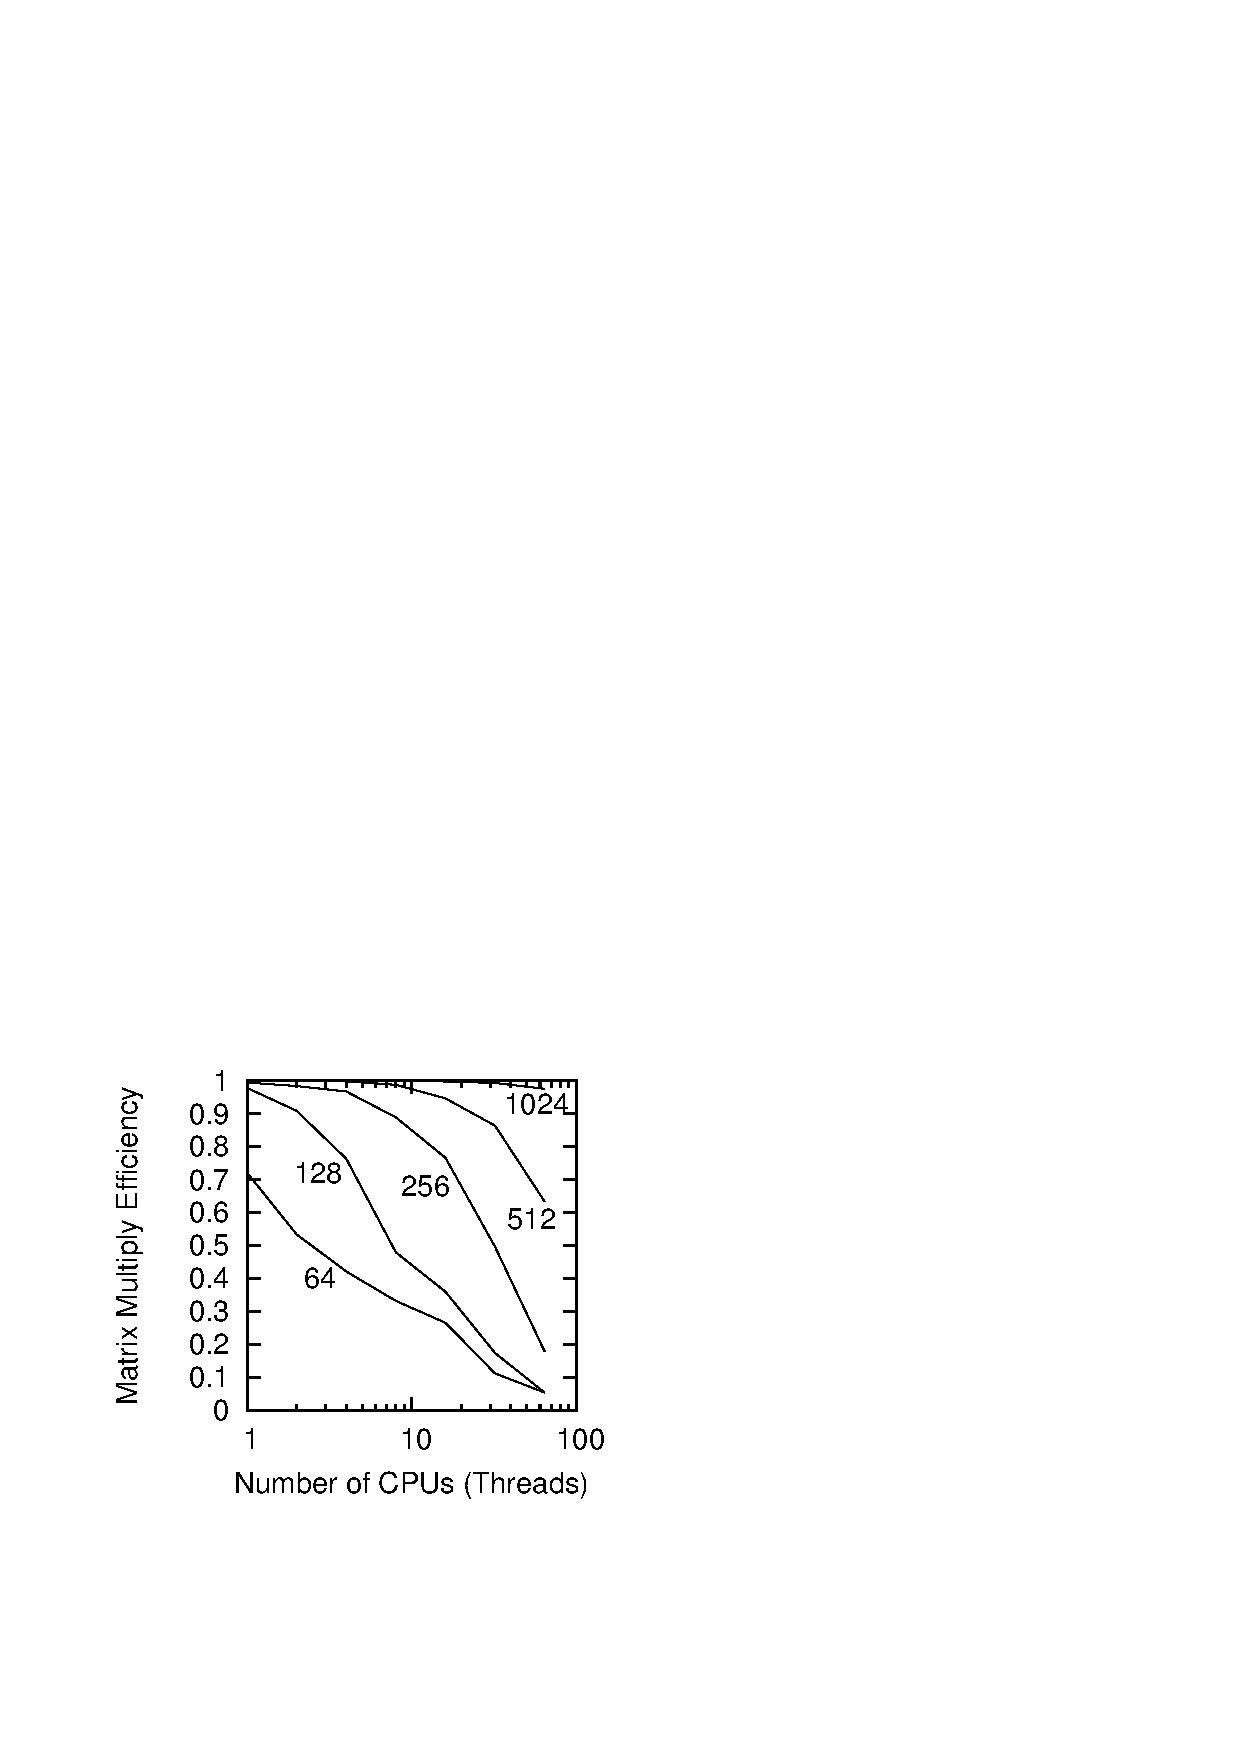
\includegraphics{SMPdesign/matmuleff}}
\end{center}
\caption{Matrix Multiply Efficiency}
\label{fig:SMPdesign:Matrix Multiply Efficiency}
\end{figure}

하지만,
Figure~\ref{fig:SMPdesign:Matrix Multiply Efficiency} 는 다르게 이야기하는데,
특히 64 행 64 열 행렬 곱셈에서는 0.7 보다 나은 효율성을 절대 갖지 못합니다,
싱글쓰레드고 동작하는데도 불구하고 말이지요.
512 행 512 열 행렬 곱셈의 효율성은 10 쓰레드 아래에서는 1.0보다 조금 작은
것으로 측정되며 심지어 1024 행 1024 열 행렬 곱셈조차도 수십 쓰레드에서는 완벽한
효율성을 벗어나게 되고 맙니다.
더도 아니고 덜도 아니고, 이 그림은 몰아서 처리하기의 성능과 확장성에서의 이점을
분명하게 보여주고 있으며, 이로 인해 당신의 돈의 가치도 알 수 있게 해줍니다.
\iffalse

However,
Figure~\ref{fig:SMPdesign:Matrix Multiply Efficiency}
tells a different story, especially for a 64-by-64 matrix multiply,
which never gets above an efficiency of about 0.7, even when running
single-threaded.
The 512-by-512 matrix multiply's efficiency is measurably less
than 1.0 on as few as 10 threads, and even the 1024-by-1024 matrix
multiply deviates noticeably from perfection at a few tens of threads.
Nevertheless, this figure clearly demonstrates the performance and
scalability benefits of batching: If you must incur synchronization
overhead, you may as well get your money's worth.
\fi

\QuickQuiz{}
	싱글쓰레드로 동작하는 64 행 64 열 행렬 곱셈이 어떻게 1.0보다 낮은
	효율성을 가질 수 있죠?
	Figure~\ref{fig:SMPdesign:Matrix Multiply Efficiency} 의 모든
	조합에서의 결과들이 한 쓰레드에서만 돌아갈 때에는 정확히 1.0 의
	효율성을 보여야 하는 거 아닌가요?
	\iffalse

	How can a single-threaded 64-by-64 matrix multiple possibly
	have an efficiency of less than 1.0?
	Shouldn't all of the traces in
	Figure~\ref{fig:SMPdesign:Matrix Multiply Efficiency}
	have efficiency of exactly 1.0 when running on only one thread?
	\fi
\QuickQuizAnswer{
	\texttt{matmul.c} 프로그램은 명시된 수의 워커 쓰레드들을 생성하므로,
	하나의 워커 쓰레드만을 생성한 경우에도 쓰레드 생성 오버헤드는 발생할 수
	있습니다.
	하나의 워커 쓰레드의 경우에 쓰레드 생성 오버헤드를 없애기 위한 변경을
	만드는 것은 독자분들의 연습문제로 남겨두겠습니다.
	\iffalse

	The \texttt{matmul.c} program creates the specified number of
	worker threads, so even the single-worker-thread case incurs
	thread-creation overhead.
	Making the changes required to optimize away thread-creation
	overhead in the single-worker-thread case is left as an
	exercise to the reader.
	\fi
} \QuickQuizEnd

이런 비효율성 아래, Section~\ref{sec:SMPdesign:Data Locking} 에서 이야기한
데이터 락킹과 같이 더 확장성 있는 방법을 생각해 보거나 다음 섹션에서 다룰 병렬
상황 빠른 수행 경로 해결책을 고려해 보는것도 가치가 있을 것입니다.
\iffalse

Given these inefficiencies,
it is worthwhile to look into more-scalable approaches
such as the data locking described in
Section~\ref{sec:SMPdesign:Data Locking}
or the parallel-fastpath approach discussed in the next section.
\fi

\QuickQuiz{}
	행렬 곱셈에서 데이터 병렬화 기법이 어떻게 도움이 될 수 있나요?
	그건 \emph{이미} 병렬적인 데이터잖아요!!!
	\iffalse

	How are data-parallel techniques going to help with matrix
	multiply?
	It is \emph{already} data parallel!!!
	\fi
\QuickQuizAnswer{
	주의를 기울이고 있으신 것 같아 기쁩니다!
	이 예는 데이터 병렬성은 매우 좋은 것이긴 하지만, 어떤 그리고 모든
	비효율성의 원인을 자동으로 제거하는 마술봉은 아니란 것을 보이기 위한
	것임을 보이기 위한 것입니다.
	64 쓰레드에게 ``한정적인'' 상황에서조차도 전체 성능을 가지고 선형적으로
	성능을 확장하는 데에는 설계와 구현의 모든 단계에서의 세심한 주의가
	필요합니다.
	\iffalse

	I am glad that you are paying attention!
	This example serves to show that although data parallelism can
	be a very good thing, it is not some magic wand that automatically
	wards off any and all sources of inefficiency.
	Linear scaling at full performance, even to ``only'' 64 threads,
	requires care at all phases of design and implementation.
	\fi

	특히, 분할된 조각의 크기에 매우 세심한 관심을 기울여야만 합니다.
	예를 들어, 64 행 64 열 행렬 곱셈 문제를 64 쓰레드에게 쪼갠다면, 각
	쓰레드는 64 개의 부동소수점 곱셈 연산만을 하게 될 것입니다.
	부동소수점 곱셈 연산의 비용은 쓰레드 생성의 오버헤드에 비하면 매우
	작습니다.

	교훈: 변화무쌍한 입력을 받을 수 있는 병렬 프로그램을 가지고 있다면,
	항상 입력의 크기를 체크하는 과정을 포함시켜서 병렬화 시킬 가치가 없을
	정도로 너무 작은 입력 사이즈에 대응하도록 하십시오.
	그리고 병렬화에 도움이 되지 않을 정도라면, 쓰레드를 생성하는데 필요한
	오버헤드를 감내하기에도 도움이 되지 않을 정도입니다, 그렇죠?
	\iffalse

	In particular, you need to pay careful attention to the
	size of the partitions.
	For example, if you split a 64-by-64 matrix multiply across
	64 threads, each thread gets only 64 floating-point multiplies.
	The cost of a floating-point multiply is miniscule compared to
	the overhead of thread creation.

	Moral: If you have a parallel program with variable input,
	always include a check for the input size being too small to
	be worth parallelizing.
	And when it is not helpful to parallelize, it is not helpful
	to incur the overhead required to spawn a thread, now is it?
	\fi
} \QuickQuizEnd

\section{Parallel Fastpath}
\label{sec:SMPdesign:Parallel Fastpath}

잘게 쪼개진 (그리고 따라서 \emph{일반적으로} 높은 성능을 갖는) 설계들은 굵게
쪼개진 설계들에 비해 일반적으로 더 복잡합니다.
많은 경우, 대부분의 오버헤드는 코드의 작은 부분에서 발생합니다~\cite{Knuth73}.
그러니 그 작은 부분에 집중하는 노력을 가져보는게 어떨까요?

이게 병렬 빠른 수행 경로 디자인 패턴을 뒷받침하는 아이디어로, 전체 알고리즘을
적극적으로 병렬화 하려 하면 요구되는 복잡성을 일으키지 않고 일반적인 경우를
위한 코드 수행 경로를 적극적으로 병렬화 시키는 것입니다.
이를 위해선 병렬화 하려는 특정 알고리즘만 이해해선 안되고, 그 알고리즘이 목표로
하는 워크로드에 대해서도 이해해야만 합니다.
병렬 빠른 수행 경로를 만들기 위해선 커다란 창조성과 설계 노력이 종종 필요하곤
합니다.

병렬 빠른 수행 경로는 서로 다른 패턴들 (하나는 빠른 수행경로를 위해, 다른
경우를 위해 또 하나) 을 조합하고 따라서 임시적 패턴입니다.
다음의 병렬 빠른 수행경로의 예들은
Figure~\ref{fig:SMPdesign:Parallel-Fastpath Design Patterns} 에 그려진 것처럼
그 자신의 패턴을 정당화 하기 충분할 만큼 자주 일어납니다:
\iffalse

Fine-grained (and therefore \emph{usually} higher-performance)
designs are typically more complex than are coarser-grained designs.
In many cases, most of the overhead is incurred by a small fraction
of the code~\cite{Knuth73}.
So why not focus effort on that small fraction?

This is the idea behind the parallel-fastpath design pattern, to aggressively
parallelize the common-case code path without incurring the complexity
that would be required to aggressively parallelize the entire algorithm.
You must understand not only the specific algorithm you wish
to parallelize, but also the workload that the algorithm will
be subjected to.  Great creativity and design
effort is often required to construct a parallel fastpath.

Parallel fastpath combines different patterns (one for the
fastpath, one elsewhere) and is therefore a template pattern.
The following instances of parallel
fastpath occur often enough to warrant their own patterns,
as depicted in Figure~\ref{fig:SMPdesign:Parallel-Fastpath Design Patterns}:
\fi

\begin{figure}[htb]
\begin{center}
% \resizebox{3in}{!}{\includegraphics{SMPdesign/ParallelFastpath}}
\includegraphics{SMPdesign/ParallelFastpath}
\end{center}
\caption{Parallel-Fastpath Design Patterns}
\label{fig:SMPdesign:Parallel-Fastpath Design Patterns}
\end{figure}

\begin{enumerate}
\item	Reader/Writer 락킹
	(아래의 Section~\ref{sec:SMPdesign:Reader/Writer Locking} 에서
	설명합니다).
\item	고성능을 위해 Reader/Writer 락킹을 대체할 수 있으며 이 챕터에서는
	더이상 설명되지 않을 Read-copy update (RCU).
\item	Section~\ref{sec:SMPdesign:Hierarchical Locking} 에서 다뤄질 계층적
	락킹~(\cite{McKenney95b}).
\item	리소스 할당자 캐시~(\cite{McKenney95b,McKenney93}).
	더 자세한 내용을 위해선
	Section~\ref{sec:SMPdesign:Resource Allocator Caches} 을 참고하십시오.
\iffalse

\item	Reader/Writer Locking
	(described below in Section~\ref{sec:SMPdesign:Reader/Writer Locking}).
\item	Read-copy update (RCU), which may be used as a high-performance
	replacement for reader/writer locking, is introduced in
	Section~\ref{sec:defer:Read-Copy Update (RCU)}, and will not
	be discussed further in this chapter.
\item   Hierarchical Locking~(\cite{McKenney95b}), which is touched upon
	in Section~\ref{sec:SMPdesign:Hierarchical Locking}.
\item	Resource Allocator Caches~(\cite{McKenney95b,McKenney93}).
	See Section~\ref{sec:SMPdesign:Resource Allocator Caches}
	for more detail.
\fi
\end{enumerate}

\subsection{Reader/Writer Locking}
\label{sec:SMPdesign:Reader/Writer Locking}

동기화 오버헤드가 무시할만 하다면 (예를 들어, 프로그램이 커다란 크리티컬
섹션들에 굵게 쪼개진 병렬성을 사용한다면), 그리고 그 크리티컬 섹션들의 작은
부분들만이 데이터를 수정한다면, 여러 읽는 작업들을 병렬로 수행될 수 있도록 하면
확장성을 크게 개선시킬 것입니다.
쓰기 작업은 읽기 작업과도, 다른 쓰기 작업들과도 배타적으로 수행되어야 합니다.
reader-writer 락킹의 많은 구현이 존재하는데,
Section~\ref{sec:toolsoftrade:POSIX Reader-Writer Locking} 에 설명된 POSIX
구현도 그 중 하나입니다.
Figure~\ref{fig:SMPdesign:Reader-Writer-Locking Hash Table Search} 는 해시
테이블이 reader-writer 락킹을 사용해 어떻게 구현될 수 있는지 보입니다.
\iffalse

If synchronization overhead is negligible (for example, if the program
uses coarse-grained parallelism with large critical sections), and if
only a small fraction of the critical sections modify data, then allowing
multiple readers to proceed in parallel can greatly increase scalability.
Writers exclude both readers and each other.
There are many implementations of reader-writer locking, including
the POSIX implementation described in
Section~\ref{sec:toolsoftrade:POSIX Reader-Writer Locking}.
Figure~\ref{fig:SMPdesign:Reader-Writer-Locking Hash Table Search}
shows how the hash search might be implemented using reader-writer locking.
\fi

\begin{figure}[htbp]
{ \scriptsize
\begin{verbatim}
  1 rwlock_t hash_lock;
  2
  3 struct hash_table
  4 {
  5   long nbuckets;
  6   struct node **buckets;
  7 };
  8
  9 typedef struct node {
 10   unsigned long key;
 11   struct node *next;
 12 } node_t;
 13
 14 int hash_search(struct hash_table *h, long key)
 15 {
 16   struct node *cur;
 17   int retval;
 18
 19   read_lock(&hash_lock);
 20   cur = h->buckets[key % h->nbuckets];
 21   while (cur != NULL) {
 22     if (cur->key >= key) {
 23       retval = (cur->key == key);
 24       read_unlock(&hash_lock);
 25       return retval;
 26     }
 27     cur = cur->next;
 28   }
 29   read_unlock(&hash_lock);
 30   return 0;
 31 }
\end{verbatim}
}
\caption{Reader-Writer-Locking Hash Table Search}
\label{fig:SMPdesign:Reader-Writer-Locking Hash Table Search}
\end{figure}

Reader/writer 락킹은 비대칭적 락킹에 대한 하나의 간단한 예입니다.
Snaman~\cite{Snaman87} 은 여러 클러스터 시스템에서 사용되는, 더 화려한 여섯개
모드의 비대칭적 락킹 디자인을 설명합니다.
일반적인 락킹과 reader-writer 락킹은 Chapter~\ref{chp:Locking} 에서 특별히
자세히 설명됩니다.
\iffalse

Reader/writer locking is a simple instance of asymmetric locking.
Snaman~\cite{Snaman87} describes a more ornate six-mode
asymmetric locking design used in several clustered systems.
Locking in general and reader-writer locking in particular is described
extensively in
Chapter~\ref{chp:Locking}.
\fi

\subsection{Hierarchical Locking}
\label{sec:SMPdesign:Hierarchical Locking}

계층적 락킹의 아이디어는 잘게 쪼개진 락을 잡는 동작을 하는 동안만 잡는 굵게
쪼개진 락을 두자는 것입니다.
Figure~\ref{fig:SMPdesign:Hierarchical-Locking Hash Table Search}
는 해시 테이블 탐색에 계층적 락킹이 어떻게 사용될 수 있을지 보여주는데, 또한 이
방법의 커다란 단점 역시 보여줍니다:
두번째 락을 잡기 위한 오버헤드를 감내했지만, 그 락은 짧은 시간동안만 잡습니다.
이 경우, 간단한 데이터 락킹 방법은 더 간단하고 더 좋은 성능을 보일 것입니다.
\iffalse

The idea behind hierarchical locking is to have a coarse-grained lock
that is held only long enough to work out which fine-grained lock
to acquire.
Figure~\ref{fig:SMPdesign:Hierarchical-Locking Hash Table Search}
shows how our hash-table search might be adapted to do hierarchical
locking, but also shows the great weakness of this approach:
we have paid the overhead of acquiring a second lock, but we only
hold it for a short time.
In this case, the simpler data-locking approach would be simpler
and likely perform better.
\fi

\begin{figure}[htbp]
{ \scriptsize
\begin{verbatim}
  1 struct hash_table
  2 {
  3   long nbuckets;
  4   struct bucket **buckets;
  5 };
  6
  7 struct bucket {
  8   spinlock_t bucket_lock;
  9   node_t *list_head;
 10 };
 11
 12 typedef struct node {
 13   spinlock_t node_lock;
 14   unsigned long key;
 15   struct node *next;
 16 } node_t;
 17
 18 int hash_search(struct hash_table *h, long key)
 19 {
 20   struct bucket *bp;
 21   struct node *cur;
 22   int retval;
 23
 24   bp = h->buckets[key % h->nbuckets];
 25   spin_lock(&bp->bucket_lock);
 26   cur = bp->list_head;
 27   while (cur != NULL) {
 28     if (cur->key >= key) {
 29       spin_lock(&cur->node_lock);
 30       spin_unlock(&bp->bucket_lock);
 31       retval = (cur->key == key);
 32       spin_unlock(&cur->node_lock);
 33       return retval;
 34     }
 35     cur = cur->next;
 36   }
 37   spin_unlock(&bp->bucket_lock);
 38   return 0;
 39 }
\end{verbatim}
}
\caption{Hierarchical-Locking Hash Table Search}
\label{fig:SMPdesign:Hierarchical-Locking Hash Table Search}
\end{figure}

\QuickQuiz{}
	계층적 락킹이 잘 동작할 만한 상황은 뭐가 있을까요?
	\iffalse

	In what situation would hierarchical locking work well?
	\fi
\QuickQuizAnswer{
	Figure~\ref{fig:SMPdesign:Hierarchical-Locking Hash Table Search} 의
	라인~31 에서의 비교 연산이 훨씬 무거운 연산으로 교체된다면, {\tt
	bp->bucket\_lock} 을 놓는 작업은 \emph{아마도} 락 경쟁을 충분히
	줄여줘서 추가적인 {\tt cur->node\_lock} 의 획득과 해제에 드는
	오버헤드보다 우세해질 수도 있을 것입니다.
	\iffalse

	If the comparison on line~31 of
	Figure~\ref{fig:SMPdesign:Hierarchical-Locking Hash Table Search}
	were replaced by a much heavier-weight operation,
	then releasing {\tt bp->bucket\_lock} \emph{might} reduce lock
	contention enough to outweigh the overhead of the extra
	acquisition and release of {\tt cur->node\_lock}.
	\fi
} \QuickQuizEnd

\subsection{Resource Allocator Caches}
\label{sec:SMPdesign:Resource Allocator Caches}

이 섹션에서는 병렬 고정 크기 블럭 메모리 얼로케이터의 단순화된 개요를
제공합니다.
더 자세한 설명은
literature~\cite{McKenney92a,McKenney93,Bonwick01slab,McKenney01e} 나
리눅스 커널~\cite{Torvalds2.6kernel} 에서 찾을 수 있습니다.
\iffalse

This section presents a simplified schematic of a parallel fixed-block-size
memory allocator.
More detailed descriptions may be found in the
literature~\cite{McKenney92a,McKenney93,Bonwick01slab,McKenney01e}
or in the Linux kernel~\cite{Torvalds2.6kernel}.
\fi

\subsubsection{Parallel Resource Allocation Problem}

병렬 메모리 할당자가 마주하는 기본적인 문제는 일반적인 경우의 매우 빠른 메모리
할당과 해제 기능을 제공해야 하는 필요와 불리한 할당 / 해제 패턴들을 마주했을 때
효과적으로 메모리를 분산시켜야 하는 필요성 사이의 갈등입니다.

이 갈등을 보기 위해, 이 문제에 데이터 소유권을 직접적으로 활용한 경우를 생각해
봅시다 --- 단순히 각 CPU 가 자기 몫을 소유하도록 메모리를 분할하는 방법입니다.
예를 들어, 두개의 CPU 를 갖고 2 기가바이트의 메모리를 갖는 시스템 (제가 바로
지금 글을 쓰고 있는 기계와 같습니다) 이라고 생각해 봅시다.
간단히 각 CPU 에 1 기가바이트씩 메모리를 할당해 주고 각 CPU 가 그 자신이
소유하고 있는 메모리 덩어리에 접근하도록 할 수 있는데, 이렇게 되면 락킹의
필요성과 복잡성, 그리고 오버헤드들이 없습니다.
불행히도, 이 간단한 계획은 간단한 생산자-소비자 워크로드 같은 경우에서 일어날
수 있는, CPU~0 이 모든 메모리를 할당받고 CPU~1 이 그걸 해제하는 알고리즘이
있다면 망가질 수 있습니다.

다른 극단적 방법인 코드 락킹의 경우에는 과한 락 경쟁과 오버헤드로 고통받게 될
수 있습니다~\cite{McKenney93}.
\iffalse

The basic problem facing a parallel memory allocator is the tension
between the need to provide extremely fast memory allocation and
freeing in the common case and the need to efficiently distribute
memory in face of unfavorable allocation and freeing patterns.

To see this tension, consider a straightforward application of
data ownership to this problem --- simply carve up memory so that
each CPU owns its share.
For example, suppose that a system with two CPUs has two gigabytes
of memory (such as the one that I am typing on right now).
We could simply assign each CPU one gigabyte of memory, and allow
each CPU to access its own private chunk of memory, without the
need for locking and its complexities and overheads.
Unfortunately, this simple scheme breaks down if an algorithm happens
to have CPU~0 allocate all of the memory and CPU~1 the free it, as
would happen in a simple producer-consumer workload.

The other extreme, code locking, suffers from excessive lock contention
and overhead~\cite{McKenney93}.
\fi

\subsubsection{Parallel Fastpath for Resource Allocation}

일반적으로 사용되는 방법은 각각의 CPU 가 적당한 캐시나 블럭들을 소유하는 병렬
빠른 수행 경로를 사용하고 추가적인 블럭들을 위한 공유 풀에는 커다란 코드 락킹을
사용해서 관리하는 방법입니다.
한 CPU 가 메모리 블럭들을 독점하는 것을 막기 위해, 각 CPU 의 캐시에 존재할 수
있는 블럭들의 갯수에 제한을 걸어 둡니다.
두개의 CPU 가 있는 시스템에서, 메모리 블럭들의 흐름은
Figure~\ref{fig:SMPdesign:Allocator Cache Schematic} 에 보여진 대로일 것입니다:
한 CPU 가 자신의 풀이 꽉 차서 블럭을 하나 해제하려고 할 때에는, 블럭들을 글로벌
풀에 보내고, 비슷하게, 그 CPU 가 자신의 풀이 비어서 블럭을 할당받으려 할 때에는
글로벌 풀로부터 블럭들을 얻어옵니다.
\iffalse

The commonly used solution uses parallel fastpath with each CPU
owning a modest cache of blocks, and with a large code-locked
shared pool for additional blocks.
To prevent any given CPU from monopolizing the memory blocks,
we place a limit on the number of blocks that can be in each CPU's
cache.
In a two-CPU system, the flow of memory blocks will be as shown
in Figure~\ref{fig:SMPdesign:Allocator Cache Schematic}:
when a given CPU is trying to free a block when its pool is full,
it sends blocks to the global pool, and, similarly, when that CPU
is trying to allocate a block when its pool is empty, it retrieves
blocks from the global pool.
\fi

\begin{figure}[htb]
\begin{center}
\resizebox{3in}{!}{\includegraphics{SMPdesign/allocatorcache}}
\end{center}
\caption{Allocator Cache Schematic}
\label{fig:SMPdesign:Allocator Cache Schematic}
\end{figure}

\subsubsection{Data Structures}

Figure~\ref{fig:SMPdesign:Allocator-Cache Data Structures} 에 할당자 캐시들의
``장난감'' 구현을 위한 실제 데이터 구조체가 있습니다.
Figure~\ref{fig:SMPdesign:Allocator Cache Schematic} 의 ``Global Pool'' 은
\co{struct globalmempool} 타입의 \co{globalmem} 으로 구현되었고 \co{struct
percpumempool} 타입의 per-CPU 변수 \co{percpumem} 으로 두개의 CPU 별 풀들이
구현되었습니다.
이 데이터 구조체들 둘 다 각자의 \co{pool} 필드 안의 블럭들로의 포인터들의
배열을 가지고 있는데, 이것들은 인덱스 0부터 위쪽으로 채워져 나갑니다.
따라서, 만약 \co{globalmem.pool[3]} 이 \co{NULL} 이라면, 인덱스 4부터 위쪽인 이
배열의 나머지들 역시 모두 \co{NULL} 이어야 합니다.
\co{cur} 필드는 \co{pool} 배열의 꽉찬 원소들 중 가장 높은 숫자의 인덱스를
갖는데, 만약 모든 원소들이 텅 비어있다면 -1을 갖습니다.
\co{globalmem.pool[0]} 부터 \co{globalmem.pool[globalmem.cur]} 사이의 모든
원소들은 반드시 꽉 차 있어야 하고, 나머지 것들은 모두 비어있어야만
합니다.\footnote{
	두 풀 사이즈 (\co{TARGET_POOL_SIZE} 와 \co{GLOBAL_POOL_SIZE}) 모두
	비현실적으로 작습니다만, 이 작은 크기가 이 프로그램의 행동이 어떻게
	이루어지는지 이해하기 위해 프로그램을 한단계씩 실행시켜 나가기 편하게
	도와줄 겁니다.}
\iffalse

The actual data structures for a ``toy'' implementation of allocator
caches are shown in
Figure~\ref{fig:SMPdesign:Allocator-Cache Data Structures}.
The ``Global Pool'' of Figure~\ref{fig:SMPdesign:Allocator Cache Schematic}
is implemented by \co{globalmem} of type \co{struct globalmempool},
and the two CPU pools by the per-CPU variable \co{percpumem} of
type \co{struct percpumempool}.
Both of these data structures have arrays of pointers to blocks
in their \co{pool} fields, which are filled from index zero upwards.
Thus, if \co{globalmem.pool[3]} is \co{NULL}, then the remainder of
the array from index 4 up must also be \co{NULL}.
The \co{cur} fields contain the index of the highest-numbered full
element of the \co{pool} array, or -1 if all elements are empty.
All elements from \co{globalmem.pool[0]} through
\co{globalmem.pool[globalmem.cur]} must be full, and all the rest
must be empty.\footnote{
	Both pool sizes (\co{TARGET_POOL_SIZE} and
	\co{GLOBAL_POOL_SIZE}) are unrealistically small, but this small
	size makes it easier to single-step the program in order to get
	a feel for its operation.}
\fi

\begin{figure}[htbp]
{ \scriptsize
\begin{verbatim}
  1 #define TARGET_POOL_SIZE 3
  2 #define GLOBAL_POOL_SIZE 40
  3
  4 struct globalmempool {
  5   spinlock_t mutex;
  6   int cur;
  7   struct memblock *pool[GLOBAL_POOL_SIZE];
  8 } globalmem;
  9
 10 struct percpumempool {
 11   int cur;
 12   struct memblock *pool[2 * TARGET_POOL_SIZE];
 13 };
 14
 15 DEFINE_PER_THREAD(struct percpumempool, percpumem);
\end{verbatim}
}
\caption{Allocator-Cache Data Structures}
\label{fig:SMPdesign:Allocator-Cache Data Structures}
\end{figure}

풀 데이터 구조체의 동작이 어떻게 될지에 대한 그림이
Figure~\ref{fig:SMPdesign:Allocator Pool Schematic} 에 있는데, 여섯개의
박스들은 \co{pool} 필드를 구성하는 포인터들의 배열을 의미하며, 그 앞의 숫자는
\co{cur} 필드를 의미합니다.
색이 칠해진 박스들은 \co{NULL} 이 아닌 포인터들을 의미하며, 비어있는 박스들은
\co{NULL} 포인터들을 의미합니다.
중요하지만 좀 혼란스러울 수도 있는 이야기입니다만 이 데이터 구조체가 항상
지키게 되는 사실 (불변식, invariant) 은, \co{cur} 필드는 항상 \co{NULL} 이 아닌
포인터들의 수보다 하나 작을 것이란 점입니다.
\iffalse

The operation of the pool data structures is illustrated by
Figure~\ref{fig:SMPdesign:Allocator Pool Schematic},
with the six boxes representing the array of pointers making up
the \co{pool} field, and the number preceding them representing
the \co{cur} field.
The shaded boxes represent non-\co{NULL} pointers, while the empty
boxes represent \co{NULL} pointers.
An important, though potentially confusing, invariant of this
data structure is that the \co{cur} field is always one
smaller than the number of non-\co{NULL} pointers.
\fi

\begin{figure}[htb]
\begin{center}
\resizebox{3in}{!}{\includegraphics{SMPdesign/AllocatorPool}}
\end{center}
\caption{Allocator Pool Schematic}
\label{fig:SMPdesign:Allocator Pool Schematic}
\end{figure}

\subsubsection{Allocation Function}

할당을 하는 함수인 \co{memblock_alloc()} 을
Figure~\ref{fig:SMPdesign:Allocator-Cache Allocator Function} 에서 확인할 수
있습니다.
Line~7 에서는 현재 쓰레드의 per-thread 풀을 가져오고, line~8 에서 그게
비어있는지 확인합니다.

만약 그렇다면, line~9-16 에서 line~9 에서 획득하고 line~16 에서 해제하는 스핀락
아래 글로벌 풀로부터 해당 per-thread 풀을 채우려 시도합니다.
Line~10-14 는 블럭들을 글로벌에서 per-thread 풀로 로컬 풀이 목표로 하는 크기
(절반) 에 도달하거나 글로벌 풀이 텅 빌 때까지 옮기고, line~15 에서는 per-thread
풀의 수를 올바른 값으로 설정합니다.

어떤 경우든, line~18 에서 per-thread 풀이 여전히 비어있는지 확인하고, 만약
그렇지 않다면, line~19-21 에서 블럭 하나를 제거하고 그걸 리턴합니다.
그렇지 않다면, line~23 에서 메모리가 부족하다는 슬픈 이야기를 전합니다.
\iffalse

The allocation function \co{memblock_alloc()} may be seen in
Figure~\ref{fig:SMPdesign:Allocator-Cache Allocator Function}.
Line~7 picks up the current thread's per-thread pool,
and line~8 check to see if it is empty.

If so, lines~9-16 attempt to refill it from the global pool
under the spinlock acquired on line~9 and released on line~16.
Lines~10-14 move blocks from the global to the per-thread pool until
either the local pool reaches its target size (half full) or
the global pool is exhausted, and line~15 sets the per-thread pool's
count to the proper value.

In either case, line~18 checks for the per-thread pool still being
empty, and if not, lines~19-21 remove a block and return it.
Otherwise, line~23 tells the sad tale of memory exhaustion.
\fi

\begin{figure}[htbp]
{ \scriptsize
\begin{verbatim}
  1 struct memblock *memblock_alloc(void)
  2 {
  3   int i;
  4   struct memblock *p;
  5   struct percpumempool *pcpp;
  6
  7   pcpp = &__get_thread_var(percpumem);
  8   if (pcpp->cur < 0) {
  9     spin_lock(&globalmem.mutex);
 10     for (i = 0; i < TARGET_POOL_SIZE &&
 11                 globalmem.cur >= 0; i++) {
 12       pcpp->pool[i] = globalmem.pool[globalmem.cur];
 13       globalmem.pool[globalmem.cur--] = NULL;
 14     }
 15     pcpp->cur = i - 1;
 16     spin_unlock(&globalmem.mutex);
 17   }
 18   if (pcpp->cur >= 0) {
 19     p = pcpp->pool[pcpp->cur];
 20     pcpp->pool[pcpp->cur--] = NULL;
 21     return p;
 22   }
 23   return NULL;
 24 }
\end{verbatim}
}
\caption{Allocator-Cache Allocator Function}
\label{fig:SMPdesign:Allocator-Cache Allocator Function}
\end{figure}

\subsubsection{Free Function}
Figure~\ref{fig:SMPdesign:Allocator-Cache Free Function} 는 메모리 블럭 해제
함수를 보입니다.
Line~6 에서는 이 쓰레드의 풀로의 포인터를 얻어오고 line~7 에서 이 per-thread
풀이 꽉 차 있는지 확인합니다.

만약 그렇다면, line~8-15 에서 이 per-thread 풀의 절반을 글로벌 풀로 비워내는데,
이 때 line~8 과 14 에서 글로벌 풀을 위한 스핀락을 각각 잡고 풉니다.
Line~9-12 에서는 로컬에서 글로벌 풀로 블럭들을 옮기는 루프를 구현하고 있으며,
line~13 에서는 per-thread 풀의 카운트를 올바른 값으로 재조정 합니다.

어떤 경우든, line~16 에서는 새로 해제된 블럭을 per-thread 풀에 넣습니다.
\iffalse

Figure~\ref{fig:SMPdesign:Allocator-Cache Free Function} shows
the memory-block free function.
Line~6 gets a pointer to this thread's pool, and
line~7 checks to see if this per-thread pool is full.

If so, lines~8-15 empty half of the per-thread pool into the global pool,
with lines~8 and 14 acquiring and releasing the spinlock.
Lines~9-12 implement the loop moving blocks from the local to the
global pool, and line~13 sets the per-thread pool's count to the proper
value.

In either case, line~16 then places the newly freed block into the
per-thread pool.
\fi

\begin{figure}[htbp]
{ \scriptsize
\begin{verbatim}
  1 void memblock_free(struct memblock *p)
  2 {
  3   int i;
  4   struct percpumempool *pcpp;
  5
  6   pcpp = &__get_thread_var(percpumem);
  7   if (pcpp->cur >= 2 * TARGET_POOL_SIZE - 1) {
  8     spin_lock(&globalmem.mutex);
  9     for (i = pcpp->cur; i >= TARGET_POOL_SIZE; i--) {
 10       globalmem.pool[++globalmem.cur] = pcpp->pool[i];
 11       pcpp->pool[i] = NULL;
 12     }
 13     pcpp->cur = i;
 14     spin_unlock(&globalmem.mutex);
 15   }
 16   pcpp->pool[++pcpp->cur] = p;
 17 }
\end{verbatim}
}
\caption{Allocator-Cache Free Function}
\label{fig:SMPdesign:Allocator-Cache Free Function}
\end{figure}

\subsubsection{Performance}

Rough performance results\footnote{
	This data was not collected in a statistically meaningful way,
	and therefore should be viewed with great skepticism and suspicion.
	Good data-collection and -reduction practice is discussed
	in Chapter~\ref{chp:Validation}.
	That said, repeated runs gave similar results, and these results
	match more careful evaluations of similar algorithms.}
are shown in
Figure~\ref{fig:SMPdesign:Allocator Cache Performance},
running on a dual-core Intel x86 running at 1GHz (4300 bogomips per CPU)
with at most six blocks allowed in each CPU's cache.
In this micro-benchmark,
each thread repeatedly allocates a group of blocks and then frees all
the blocks in that group, with
the number of blocks in the group being the ``allocation run length''
displayed on the x-axis.
The y-axis shows the number of successful allocation/free pairs per
microsecond --- failed allocations are not counted.
The ``X''s are from a two-thread run, while the ``+''s are from a
single-threaded run.

\begin{figure}[htb]
\begin{center}
\resizebox{3in}{!}{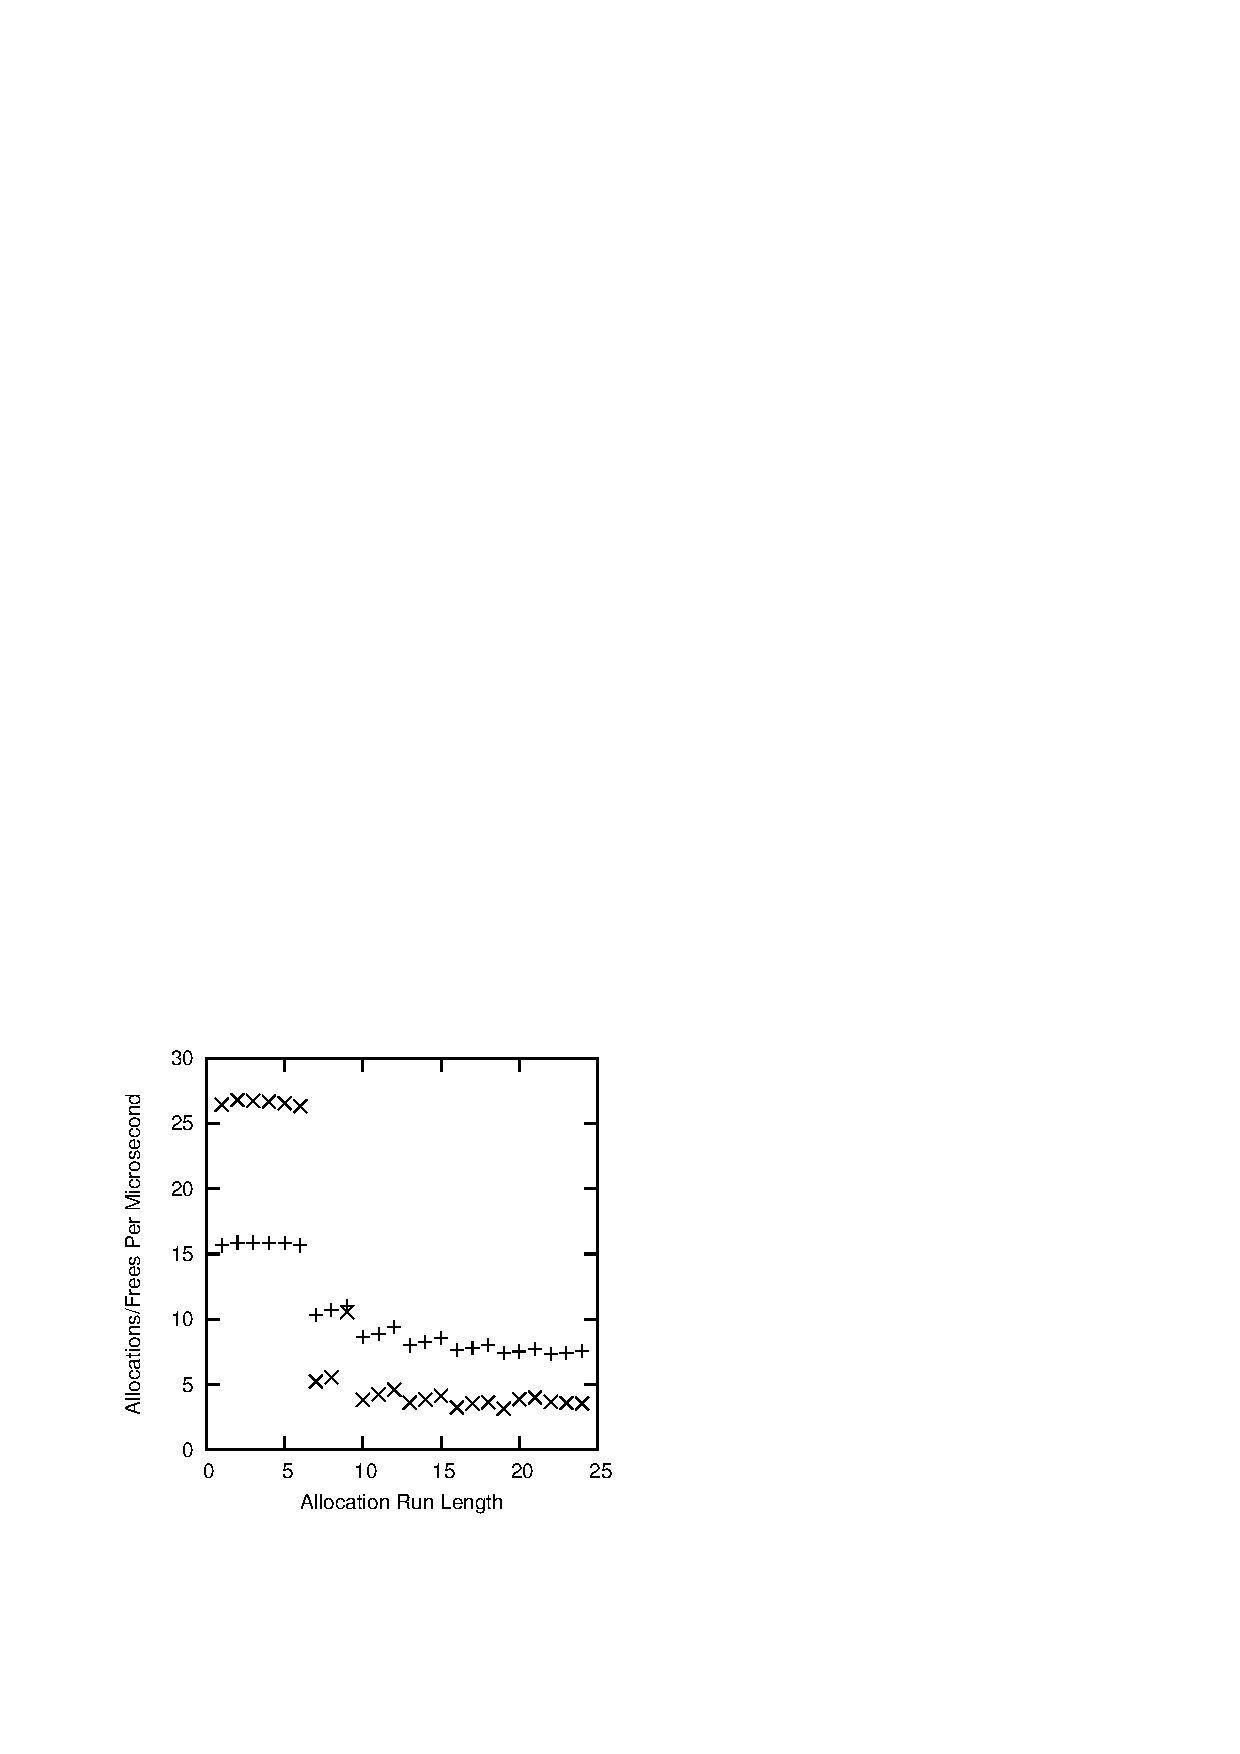
\includegraphics{SMPdesign/smpalloc}}
\end{center}
\caption{Allocator Cache Performance}
\label{fig:SMPdesign:Allocator Cache Performance}
\end{figure}

Note that run lengths up to six scale linearly and give excellent performance,
while run lengths greater than six show poor performance and almost always
also show \emph{negative} scaling.
It is therefore quite important to size \co{TARGET_POOL_SIZE}
sufficiently large,
which fortunately is usually quite easy to do in actual
practice~\cite{McKenney01e}, especially given today's large memories.
For example, in most systems, it is quite reasonable to set
\co{TARGET_POOL_SIZE} to 100, in which case allocations and frees
are guaranteed to be confined to per-thread pools at least 99\% of
the time.

As can be seen from the figure, the situations where the common-case
data-ownership applies (run lengths up to six) provide greatly improved
performance compared to the cases where locks must be acquired.
Avoiding synchronization in the common case will be a recurring theme through
this book.

\QuickQuiz{}
	In Figure~\ref{fig:SMPdesign:Allocator Cache Performance},
	there is a pattern of performance rising with increasing run
	length in groups of three samples, for example, for run lengths
	10, 11, and 12.
	Why?
\QuickQuizAnswer{
	This is due to the per-CPU target value being three.
	A run length of 12 must acquire the global-pool lock twice,
	while a run length of 13 must acquire the global-pool lock
	three times.
} \QuickQuizEnd

\QuickQuiz{}
	Allocation failures were observed in the two-thread
	tests at run lengths of 19 and greater.
	Given the global-pool size of 40 and the per-thread target
	pool size $s$ of three, number of threads $n$ equal to two,
	and assuming that the per-thread pools are initially
	empty with none of the memory in use, what is the smallest allocation
	run length $m$ at which failures can occur?
	(Recall that each thread repeatedly allocates $m$ block of memory,
	and then frees the $m$ blocks of memory.)
	Alternatively, given $n$ threads each with pool size $s$, and
	where each thread repeatedly first allocates $m$ blocks of memory
	and then frees those $m$ blocks, how large must the global pool
	size be?
	\emph{Note:} Obtaining the correct answer will require you to
	examine the \co{smpalloc.c} source code, and very likely
	single-step it as well.
	You have been warned!
\QuickQuizAnswer{
	This solution is adapted from one put forward by Alexey Roytman.
	It is based on the following definitions:

	\begin{description}
	\item[$g$]	Number of blocks globally available.
	\item[$i$]	Number of blocks left in the initializing thread's
			per-thread pool.  (This is one reason you needed
			to look at the code!)
	\item[$m$]	Allocation/free run length.
	\item[$n$]	Number of threads, excluding the initialization thread.
	\item[$p$]	Per-thread maximum block consumption, including
			both the blocks actually allocated and the blocks
			remaining in the per-thread pool.
	\end{description}

	The values $g$, $m$, and $n$ are given.  The value for $p$ is
	$m$ rounded up to the next multiple of $s$, as follows:

	\begin{equation}
		p = s \left \lfloor \frac{m + s - 1}{s} \right \rfloor
	\label{sec:SMPdesign:p}
	\end{equation}

	The value for $i$ is as follows:

	\begin{equation}
		i = \left \{
			\begin{array}{l}
				g \pmod{2 s} = 0: 2 s \\
				g \pmod{2 s} \ne 0: g \pmod{2 s}
			\end{array}
		    \right .
	\label{sec:SMPdesign:i}
	\end{equation}

	\begin{figure}[tb]
	\begin{center}
	\resizebox{3in}{!}{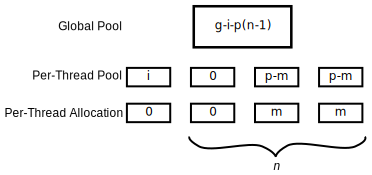
\includegraphics{SMPdesign/smpalloclim}}
	\end{center}
	\caption{Allocator Cache Run-Length Analysis}
	\label{fig:SMPdesign:Allocator Cache Run-Length Analysis}
	\end{figure}

	The relationships between these quantities is shown in
	Figure~\ref{fig:SMPdesign:Allocator Cache Run-Length Analysis}.
	The global pool is shown on the top of this figure, and
	the ``extra'' initializer thread's per-thread pool and
	per-thread allocations are the left-most pair of boxes.
	The initializer thread has no blocks allocated, but has
	$i$ blocks stranded in its per-thread pool.
	The rightmost two pairs of boxes are the per-thread pools and
	per-thread allocations of threads holding the maximum possible
	number of blocks, while the second-from-left pair of boxes
	represents the thread currently trying to allocate.

	The total number of blocks is $g$, and adding up the per-thread
	allocations and per-thread pools, we see that the global pool
	contains $g-i-p(n-1)$ blocks.
	If the allocating thread is to be successful, it needs at least
	$m$ blocks in the global pool, in other words:

	\begin{equation}
		g - i - p(n - 1) \ge m
	\label{sec:SMPdesign:g-vs-m}
	\end{equation}

	The question has $g=40$, $s=3$, and $n=2$.
	Equation~\ref{sec:SMPdesign:i} gives $i=4$, and
	Equation~\ref{sec:SMPdesign:p} gives $p=18$ for $m=18$
	and $p=21$ for $m=19$.
	Plugging these into Equation~\ref{sec:SMPdesign:g-vs-m}
	shows that $m=18$ will not overflow, but that $m=19$ might
	well do so.

	The presence of $i$ could be considered to be a bug.
	After all, why allocate memory only to have it stranded in
	the initialization thread's cache?
	One way of fixing this would be to provide a \co{memblock_flush()}
	function that flushed the current thread's pool into the
	global pool.
	The initialization thread could then invoke this function
	after freeing all of the blocks.
} \QuickQuizEnd

\subsubsection{Real-World Design}

The toy parallel resource allocator was quite simple, but real-world
designs expand on this approach in a number of ways.

First, real-world allocators are required to handle a wide range
of allocation sizes, as opposed to the single size shown in this
toy example.
One popular way to do this is to offer a fixed set of sizes, spaced
so as to balance external and internal fragmentation, such as in
the late-1980s BSD memory allocator~\cite{McKusick88}.
Doing this would mean that the ``globalmem'' variable would need
to be replicated on a per-size basis, and that the associated
lock would similarly be replicated, resulting in data locking
rather than the toy program's code locking.

Second, production-quality systems must be able to repurpose memory,
meaning that they must be able to coalesce blocks into larger structures,
such as pages~\cite{McKenney93}.
This coalescing will also need to be protected by a lock, which again
could be replicated on a per-size basis.

Third, coalesced memory must be returned to the underlying memory
system, and pages of memory must also be allocated from the underlying
memory system.
The locking required at this level will depend on that of the underlying
memory system, but could well be code locking.
Code locking can often be tolerated at this level, because this
level is so infrequently reached in well-designed systems~\cite{McKenney01e}.

Despite this real-world design's greater complexity, the underlying
idea is the same --- repeated application of parallel fastpath,
as shown in
Table~\ref{fig:app:questions:Schematic of Real-World Parallel Allocator}.

\begin{table}[htbp]
{ \scriptsize
\begin{tabular}{l|l|p{1in}}
Level	& Locking & Purpose \\
\hline
Per-thread pool	  & Data ownership & High-speed allocation \\
Global block pool & Data locking   & Distributing blocks among threads \\
Coalescing	  & Data locking   & Combining blocks into pages \\
System memory	  & Code locking   & Memory from/to system \\
\end{tabular}
}
\caption{Schematic of Real-World Parallel Allocator}
\label{fig:app:questions:Schematic of Real-World Parallel Allocator}
\end{table}

% beyond.tex

\section{Beyond Partitioning}
\label{sec:SMPdesign:Beyond Partitioning}
\OriginallyPublished{Section}{sec:SMPdesign:Beyond Partitioning}{Retrofitted Parallelism Considered Grossly Sub-Optimal}{4\textsuperscript{th} USENIX Workshop on Hot Topics on Parallelism}{PaulEMcKenney2012HOTPARsuboptimal}

이 챕터에서는 데이터 파티셔닝이 간단한 선형적으로 확장 가능한 병렬 프로그램을
설계하는데 사용될 수 있는지 알아봤습니다.
Section~\ref{sec:SMPdesign:Data Ownership} 에서는 데이터 복사 가능성에서 힌트를
얻었는데, 이는 Section~\ref{sec:defer:Read-Copy Update (RCU)} 에서 커다란
효과를 가져올 것입니다.

파티셔닝과 복사본 사용을 적용하는 주요 목표는 선형적인 속도 향상을 얻기 위한
것으로, 달리 말하자면 CPU 나 쓰레드의 수가 늘어남에 따라 전체적으로 필요한 일의
양이 크게 늘어나지는 않음을 보장하기 위한 것입니다.
파티셔닝과 복사본 사용을 통해 해결될 수 있어서 선형적인 속도향상이 가능한
문제들은 \emph{당혹스럽게 병렬적} 입니다.
하지만 이보다 더 잘할 수는 없을까요?
\iffalse

This chapter has discussed how data partitioning can be used to design
simple linearly scalable parallel programs.
Section~\ref{sec:SMPdesign:Data Ownership} hinted at the possibilities
of data replication, which will be used to great effect in
Section~\ref{sec:defer:Read-Copy Update (RCU)}.

The main goal of applying partitioning and replication is to achieve
linear speedups, in other words, to ensure that the total amount of
work required does not increase significantly as the number of CPUs
or threads increases.
A problem that can be solved via partitioning and/or replication,
resulting in linear speedups, is \emph{embarrassingly parallel}.
But can we do better?
\fi

이 질문에 답을 하기 위해, 미궁과 미로의 해결책을 생각해 보도록 합시다.
물론, 미궁과 미로는 수천년동안 매력적인 것이었으며~\cite{WikipediaLabyrinth},
따라서 그것들이 바이오 컴퓨터~\cite{AndrewAdamatzky2011SlimeMold},
GPGPU~\cite{ChristerEricson2008GPUMaze}, 심지어는 분리된
하드웨어~\cite{MIT:TRMag:MemristorMazes} 등의 컴퓨터들을 사용해서 만들어지고
해결되었음은 별로 놀라운 일도 아닙니다.
미로의 병렬적 해결책은 대학 수업에서의 과제
프로젝트~\cite{ETHZurich:FS2011maze,UMD:CMSC433maze} 로도 사용되었고, 병렬
프로그래밍 프레임웍의 이점을 보이기 위한 매개물~\cite{RonFosner2010maze} 로도
사용되었습니다.
\iffalse

To answer this question, let us examine the solution of
labyrinths and mazes.
Of course, labyrinths and mazes have been objects of fascination for
millennia~\cite{WikipediaLabyrinth},
so it should come as no surprise that they are generated and solved
using computers, including biological
computers~\cite{AndrewAdamatzky2011SlimeMold},
GPGPUs~\cite{ChristerEricson2008GPUMaze}, and even
discrete hardware~\cite{MIT:TRMag:MemristorMazes}.
Parallel solution of mazes is sometimes used as a class project in
universities~\cite{ETHZurich:FS2011maze,UMD:CMSC433maze} and
as a vehicle to demonstrate the benefits of parallel-programming
frameworks~\cite{RonFosner2010maze}.
\fi

흔한 조언은 병렬 일거리-대기열 알고리즘(PWQ: Parallel work-queue
algorithm)~\cite{ETHZurich:FS2011maze,RonFosner2010maze} 을 사용하라는
것입니다.
이 섹션은 무작위적으로 생성된 정사각형 미로를 푸는 모든 경우에 대해
순차적 알고리즘 (SEQ:SEQuential algorithm) 과 대안적인 병렬 알고리즘, 그리고
PWQ 를 비교하는 것으로 이 조언을 평가해 보겠습니다.
Section~\ref{sec:SMPdesign:Work-Queue Parallel Maze Solver} 에서는 PWQ 를
이야기 하고,
Section~\ref{sec:SMPdesign:Alternative Parallel Maze Solver} 에서 대안적인 병렬
알고리즘을 설명하며,
Section~\ref{sec:SMPdesign:Performance Comparison I} 에서는 그것의 문제 있는
성능에 대해 이야기 한 후,
Section~\ref{sec:SMPdesign:Alternative Sequential Maze Solver} 에서 앞의 대안적
병렬 알고리즘으로부터 향상된 순차적 알고리즘을 소개하며,
Section~\ref{sec:SMPdesign:Performance Comparison II} 에서 성능을 비교해 보고,
마지막으로
Section~\ref{sec:SMPdesign:Future Directions and Conclusions} 에서 미래의
방향을 알아보고 결론을 내려봅니다.
\iffalse

Common advice is to use a parallel work-queue algorithm
(PWQ)~\cite{ETHZurich:FS2011maze,RonFosner2010maze}.
This section evaluates this advice by comparing PWQ
against a sequential algorithm (SEQ) and also against
an alternative parallel algorithm, in all cases solving randomly generated
square mazes.
Section~\ref{sec:SMPdesign:Work-Queue Parallel Maze Solver} discusses PWQ,
Section~\ref{sec:SMPdesign:Alternative Parallel Maze Solver} discusses an alternative
parallel algorithm,
Section~\ref{sec:SMPdesign:Performance Comparison I} analyzes its anomalous performance,
Section~\ref{sec:SMPdesign:Alternative Sequential Maze Solver} derives an improved
sequential algorithm from the alternative parallel algorithm,
Section~\ref{sec:SMPdesign:Performance Comparison II} makes further performance
comparisons,
and finally
Section~\ref{sec:SMPdesign:Future Directions and Conclusions}
presents future directions and concluding remarks.
\fi

\subsection{Work-Queue Parallel Maze Solver}
\label{sec:SMPdesign:Work-Queue Parallel Maze Solver}

\begin{listing}[tbp]
{ \scriptsize
\begin{verbbox}
  1 int maze_solve(maze *mp, cell sc, cell ec)
  2 {
  3   cell c = sc;
  4   cell n;
  5   int vi = 0;
  6 
  7   maze_try_visit_cell(mp, c, c, &n, 1);
  8   for (;;) {
  9     while (!maze_find_any_next_cell(mp, c, &n)) {
 10       if (++vi >= mp->vi)
 11         return 0;
 12       c = mp->visited[vi].c;
 13     }
 14     do {
 15       if (n == ec) {
 16         return 1;
 17       }
 18       c = n;
 19     } while (maze_find_any_next_cell(mp, c, &n));
 20     c = mp->visited[vi].c;
 21   }
 22 }
\end{verbbox}
}
\centering
\theverbbox
\caption{SEQ Pseudocode}
\label{lst:SMPdesign:SEQ Pseudocode}
\end{listing}

PWQ 는 Listing~\ref{lst:SMPdesign:SEQ Pseudocode}(\co{maze_seq.c}) 에 있는 SEQ
에 기반합니다.
미로는 셀들의 2D 배열과 \co{->visited} 로 이름 붙여진 선형적 배열 기반 일거리
대기열로 나타내어집니다.

Line~7 에서 첫번째 셀에 들어가고, line~8-21 에 있는 루프의 매 반복에서 하나의
셀에 의해 향해지는 통로를 횡단합니다.
Line9-13 의 루프에서는 \co{->visited[]} 배열을 방문되지 않은 이웃을 가지고
방문된 셀을 위해 스캔하고, line~14-19 의 루프에서는 그 이웃을 통해 향해지는
작은 미로를 횡단합니다.
Line~20 에서는 밖의 루프에 의해 통과될 다음 경로를 위해 초기화를 합니다.
\iffalse

PWQ is based on SEQ, which is shown in
Listing~\ref{lst:SMPdesign:SEQ Pseudocode}
(\path{maze_seq.c}).
The maze is represented by a 2D array of cells and
a linear-array-based work queue named \co{->visited}.

Line~7 visits the initial cell, and each iteration of the loop spanning
lines~8-21 traverses passages headed by one cell.
The loop spanning lines~9-13 scans the \co{->visited[]} array for a
visited cell with an unvisited neighbor, and the loop spanning
lines~14-19 traverses one fork of the submaze headed by that neighbor.
Line~20 initializes for the next pass through the outer loop.
\fi

\begin{listing}[tbp]
{ \scriptsize
\begin{verbbox}
  1 int maze_try_visit_cell(struct maze *mp, cell c, cell t,
  2                         cell *n, int d)
  3 {
  4   if (!maze_cells_connected(mp, c, t) ||
  5       (*celladdr(mp, t) & VISITED))
  6     return 0;
  7   *n = t;
  8   mp->visited[mp->vi] = t;
  9   mp->vi++;
 10   *celladdr(mp, t) |= VISITED | d;
 11   return 1;
 12 }
 13 
 14 int maze_find_any_next_cell(struct maze *mp, cell c,
 15                             cell *n)
 16 {
 17   int d = (*celladdr(mp, c) & DISTANCE) + 1;
 18 
 19   if (maze_try_visit_cell(mp, c, prevcol(c), n, d))
 20     return 1;
 21   if (maze_try_visit_cell(mp, c, nextcol(c), n, d))
 22     return 1;
 23   if (maze_try_visit_cell(mp, c, prevrow(c), n, d))
 24     return 1;
 25   if (maze_try_visit_cell(mp, c, nextrow(c), n, d))
 26     return 1;
 27   return 0;
 28 }
\end{verbbox}
}
\centering
\theverbbox
\caption{SEQ Helper Pseudocode}
\label{lst:SMPdesign:SEQ Helper Pseudocode}
\end{listing}

\co{maze_try_visit_cell()} 의 슈도코드가
Listing~\ref{lst:SMPdesign:SEQ Helper Pseudocode}
(\co{maze.c}) 의 line~1-12 에 나타나
있습니다.
Line~4 에서셀 \co{c} 와 \co{n} 이 근처에 있고 연결되어 있는지 체크해 보고,
line~5 에서는 셀 \co{n} 이 아직 방문되지 않았는지 확인해 봅니다.
\co{celladdr()} 함수는 지목된 셀의 주소를 리턴합니다.
두 체크 중 하나라도 실패하면, line~6 에서 실패했음을 리턴합니다.
Line~7 에서는 다음 셀을 알리고, line~8 에서 이 셀을 \co{->visited[]} 배열의
다음 슬롯에 기록해 두고, line~9 에서 이 슬롯이 이제 채워졌음을 알리며, line~10
에서 이 셀을 방문되었음으로 마크하고 미로의 시작점으로부터의 거리를 기록해
둡니다.
Line~11 은 이제 성공했음을 리턴합니다.

\co{maze_find_any_next_cell()} 의 슈도코드가
Listing~\ref{lst:SMPdesign:SEQ Helper Pseudocode}
(\co{maze.c}) 의 line~14-28 에 있습니다.
Line~17 에서는 현재 셀의 거리 더하기 1을 얻어오고, 라인~19, 21, 23, 25 에서는
각 방향의 해당 셀들을 체크하고, ine~20, 22, 24, 26 에서는 연관된 셀이 다음 셀
후보라면 \co{true} 를 리턴합니다.
\co{prevcol()}, \co{nextcol()}, \co{prevrow()}, 그리고 \co{nextrow()} 는 각각
배열 인덱스 변환 작업을 수행합니다.
어떤 셀도 후보가 아니라면, line~27 에서 \co{false} 를 리턴합니다.
\iffalse

The pseudocode for \co{maze_try_visit_cell()} is shown on lines~1-12
of Listing~\ref{lst:SMPdesign:SEQ Helper Pseudocode}
(\path{maze.c}).
Line~4 checks to see if cells \co{c} and \co{t} are adjacent and connected,
while line~5 checks to see if cell \co{t} has not yet been visited.
The \co{celladdr()} function returns the address of the specified cell.
If either check fails, line~6 returns failure.
Line~7 indicates the next cell, line~8 records this cell in the next
slot of the \co{->visited[]} array, line~9 indicates that this slot
is now full, and line~10 marks this cell as visited and also records
the distance from the maze start.  Line~11 then returns success.

The pseudocode for \co{maze_find_any_next_cell()} is shown on lines~14-28
of Listing~\ref{lst:SMPdesign:SEQ Helper Pseudocode}
(\path{maze.c}).
Line~17 picks up the current cell's distance plus 1,
while lines~19, 21, 23, and~25
check the cell in each direction, and lines~20, 22, 24, and~26
return true if the corresponding cell is a candidate next cell.
The \co{prevcol()}, \co{nextcol()}, \co{prevrow()}, and \co{nextrow()}
each do the specified array-index-conversion operation.
If none of the cells is a candidate, line~27 returns false.
\fi

\begin{figure}[tb]
\centering
\resizebox{1.2in}{!}{\includegraphics{SMPdesign/MazeNumberPath}}
\caption{Cell-Number Solution Tracking}
\label{fig:SMPdesign:Cell-Number Solution Tracking}
\end{figure}

해당 경로는 Figure~\ref{fig:SMPdesign:Cell-Number Solution Tracking} 에
보여지는 것처럼, 미로에 시작점으로부터의 셀들의 수를 세는 것으로 기록되는데,
시작 셀은 좌상단에 위치해 있고 끝의 셀은 우하단에 위치해 있습니다.
끝 셀로부터 시작해서 연속적으로 줄어드는 셀 숫자들을 따라가는 것으로 해결
경로를 따라 횡단할 수 있습니다.
\iffalse

The path is recorded in the maze by counting the number of cells from
the starting point, as shown in
Figure~\ref{fig:SMPdesign:Cell-Number Solution Tracking},
where the starting cell is in the upper left and the ending cell is
in the lower right.
Starting at the ending cell and following
consecutively decreasing cell numbers traverses the solution.
\fi

\begin{figure}[tb]
\centering
\resizebox{2.2in}{!}{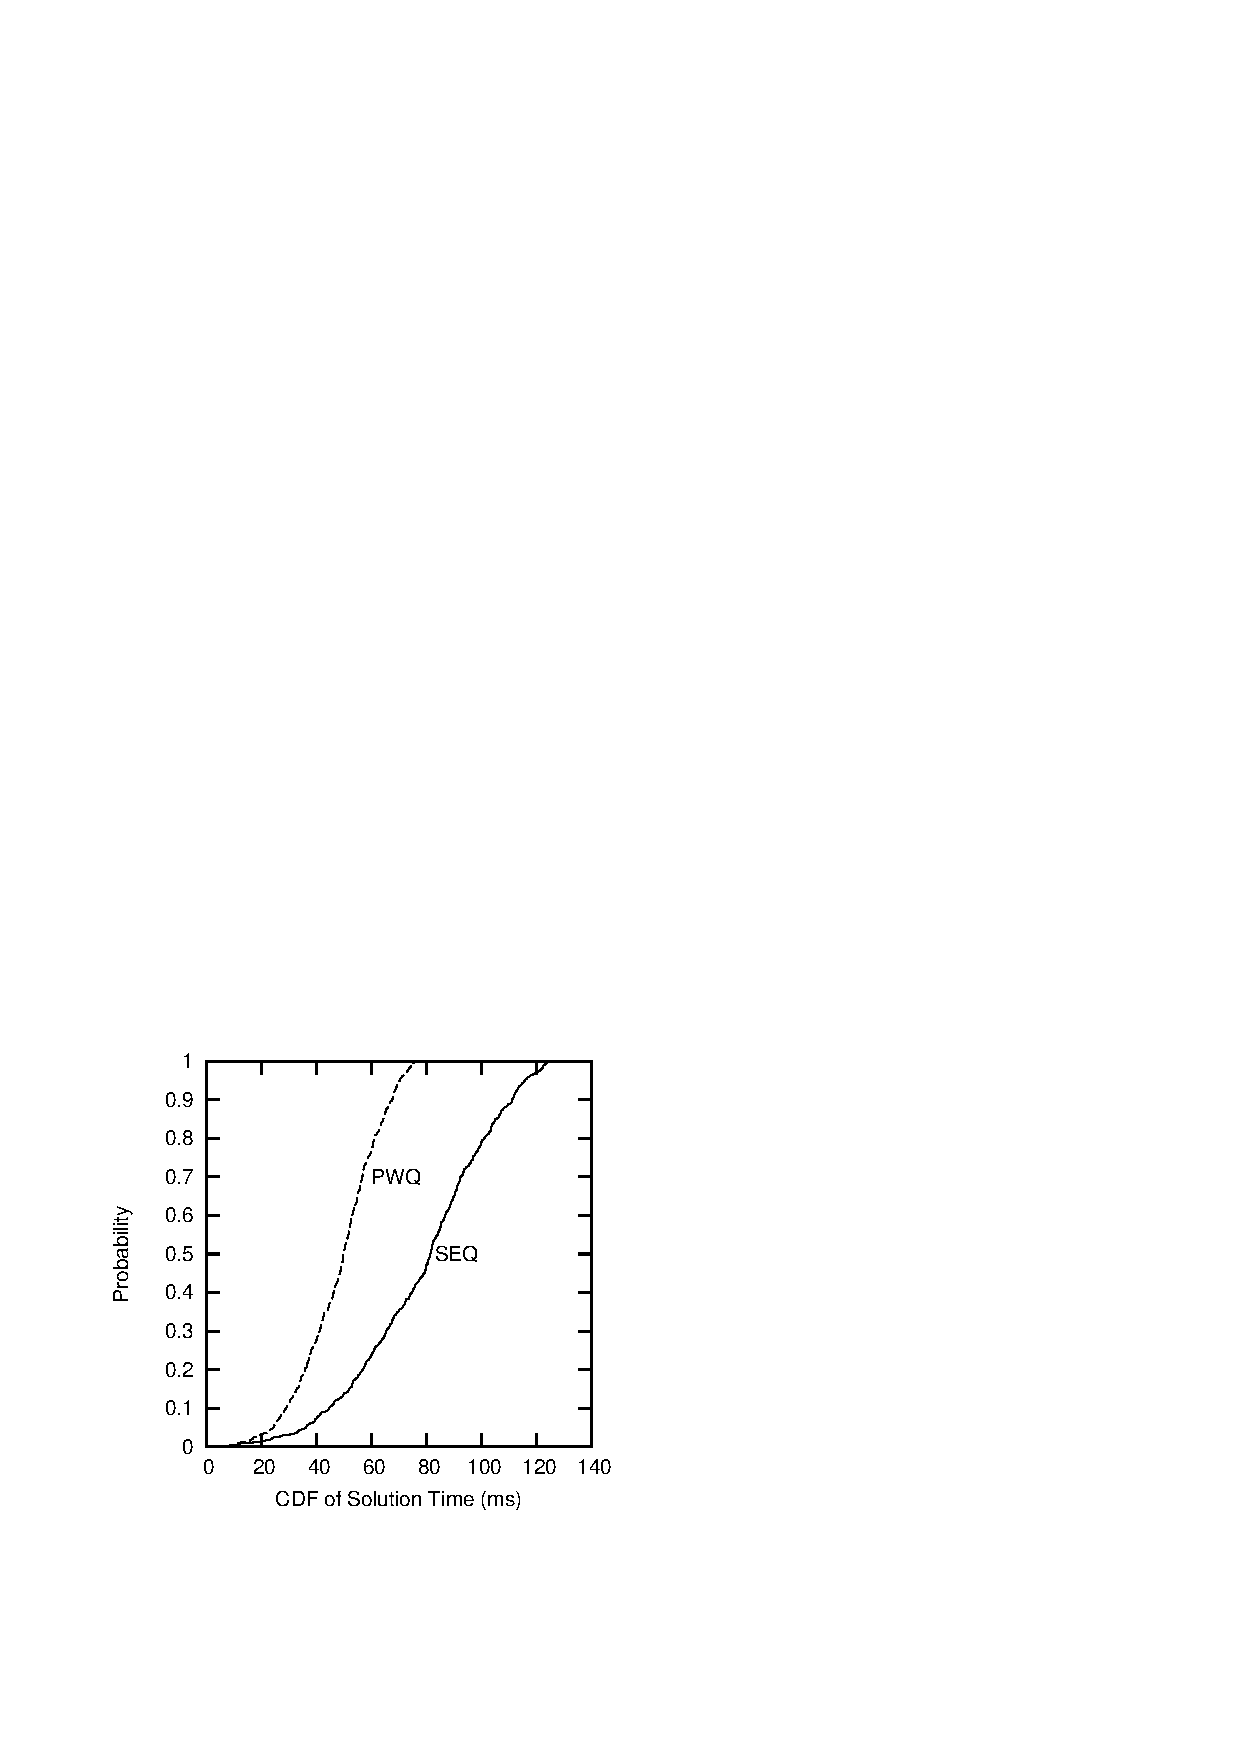
\includegraphics{SMPdesign/500-ms_seq_fg-cdf}}
\caption{CDF of Solution Times For SEQ and PWQ}
\label{fig:SMPdesign:CDF of Solution Times For SEQ and PWQ}
\end{figure}

병렬 작업 대기열 처리자 (work-queue solver) 는
Listing~\ref{lst:SMPdesign:SEQ Pseudocode} 와
~\ref{lst:SMPdesign:SEQ Helper Pseudocode} 에 보여진 알고리즘의 직선적인
병렬화입니다.
Listing~\ref{lst:SMPdesign:SEQ Pseudocode} 의 line~10 은 fetch-and-add 를
사용해야만 하고 지역 변수인 \co{vi} 는 여러 쓰레드들 사이에 공유되어야만
합니다.
Listing~\ref{lst:SMPdesign:SEQ Helper Pseudocode} 의 Line~5 와~10 은 CAS 루프로
구성되어야만 하는데, 이 때 CAS 의 실패는 미로 루프를 의미하게 됩니다.
이 그림의 Line~8-9 는 셀들을 \co{->visited[]} 배열에 동시적으로 기록하려
시도하는 것을 처리하기 위해 fetch-and-add 를 사용해야만 합니다.
\iffalse

The parallel work-queue solver is a straightforward parallelization
of the algorithm shown in
Listings~\ref{lst:SMPdesign:SEQ Pseudocode} and~\ref{lst:SMPdesign:SEQ Helper Pseudocode}.
Line~10 of Listing~\ref{lst:SMPdesign:SEQ Pseudocode} must use fetch-and-add,
and the local variable \co{vi} must be shared among the various threads.
Lines~5 and~10 of Listing~\ref{lst:SMPdesign:SEQ Helper Pseudocode} must be
combined into a CAS loop, with CAS failure indicating a loop in the
maze.
Lines~8-9 of this listing must use fetch-and-add to arbitrate concurrent
attempts to record cells in the \co{->visited[]} array.
\fi

이 접근법은 Figure~\ref{fig:SMPdesign:CDF of Solution Times For SEQ and PWQ}
에서 볼 수 있듯이 2.53GHz 의 속도로 동작하는 dual-CPU
Lenovo\textsuperscript\texttrademark W500 에서 상당한 속도 향상을 보여주는데,
두 알고리즘의 해결책을 얻는데 걸리는 시간의 누적 분포 함수들 (CDF) 을 500 개의
다른 500행 500열의 정사각으로 무작위적으로 만들어진 미로들에 대해
측정되었습니다.
이 CDF 들을 x 축에 투영해서 만들어지는 실질적인 겹쳐진 모습은
Section~\ref{sec:SMPdesign:Performance Comparison I} 에서 다루어질 것입니다.

상당히 흥미롭게도, 순차적인 해결책의 경로 탐색은 병렬 알고리즘에서도 바뀌지
않았습니다.
하지만, 이는 병렬 알고리즘의 상당한 약점을 드러냈습니다:
어떤 주어진 시간 동안 최대 하나의 쓰레드만이 해결책 경로로의 진행을 만들 수
있습니다.
이 약점은 다음 섹션에서 다루어집니다.
\iffalse


This approach does provide significant speedups on a dual-CPU
Lenovo\mytexttrademark\ W500
running at 2.53\,GHz, as shown in
Figure~\ref{fig:SMPdesign:CDF of Solution Times For SEQ and PWQ},
which shows the cumulative distribution functions (CDFs) for the solution
times of the two algorithms, based on the solution of 500 different square
500-by-500 randomly generated mazes.
The substantial overlap
of the projection of the CDFs onto the x-axis will be addressed in
Section~\ref{sec:SMPdesign:Performance Comparison I}.

Interestingly enough, the sequential solution-path tracking works unchanged
for the parallel algorithm.
However, this uncovers a significant weakness in the parallel algorithm:
At most one thread may be making progress along the solution path at
any given time.
This weakness is addressed in the next section.
\fi

\subsection{Alternative Parallel Maze Solver}
\label{sec:SMPdesign:Alternative Parallel Maze Solver}

유용한 미로 풀기 방법들은 종종 양 끝에서 시작할 것을 주장했고, 이런 조언은
자동화된 미로 해법~\cite{UMD:CMSC433maze} 의 맥락에서 최근들어 더
반복되었습니다.
이 조언은 파티셔닝과 같은 것으로, 파티셔닝은 병렬 프로그래밍의 맥락에서
운영체제 커널에 대해서도~\cite{Beck85,Inman85} 어플리케이션에
대해서도~\cite{DavidAPatterson2010TroubleMulticore} 강력한 병렬화 전략이
되어왔습니다.
이 섹션에서는 이 전략을 적용해 보는데, 해결책 경로의 양 끝단에서 시작하는
두개의 자식 쓰레드를 사용하고, 성능과 확장성에 대해 짧게 결과를 알아봅니다.
\iffalse

Youthful maze solvers are often urged to start at both ends, and
this advice has been repeated more recently in the context of automated
maze solving~\cite{UMD:CMSC433maze}.
This advice amounts to partitioning, which has been a powerful
parallelization strategy
in the context of parallel programming for both operating-system
kernels~\cite{Beck85,Inman85} and
applications~\cite{DavidAPatterson2010TroubleMulticore}.
This section applies this strategy, using two child threads that start
at opposite ends of the solution path, and takes a brief look at the
performance and scalability consequences.
\fi

\begin{listing}[tbp]
{ \scriptsize
\begin{verbbox}
  1 int maze_solve_child(maze *mp, cell *visited, cell sc)
  2 {
  3   cell c;
  4   cell n;
  5   int vi = 0;
  6 
  7   myvisited = visited; myvi = &vi;
  8   c = visited[vi];
  9   do {
 10     while (!maze_find_any_next_cell(mp, c, &n)) {
 11       if (visited[++vi].row < 0)
 12         return 0;
 13       if (ACCESS_ONCE(mp->done))
 14         return 1;
 15       c = visited[vi];
 16     }
 17     do {
 18       if (ACCESS_ONCE(mp->done))
 19         return 1;
 20       c = n;
 21     } while (maze_find_any_next_cell(mp, c, &n));
 22     c = visited[vi];
 23   } while (!ACCESS_ONCE(mp->done));
 24   return 1;
 25 }
\end{verbbox}
}
\centering
\theverbbox
\caption{Partitioned Parallel Solver Pseudocode}
\label{lst:SMPdesign:Partitioned Parallel Solver Pseudocode}
\end{listing}

Listing~\ref{lst:SMPdesign:Partitioned Parallel Solver Pseudocode}
(\co{maze_part.c}) 에 보여진 파티션을 사용한 병렬 알고리즘 (PART) 는 SEQ 와
비슷하지만 몇가지 중요한 차이점이 있습니다.
첫번째로, 각 자식 쓰레드는 자신의 \co{visited} 배열을 가지고 있는데, line~1
에서 보듯이 부모로부터 전달받은 것으로, 모두 [-1,-1] 로 초기화 되어 있어야만
합니다.
Line~7 에서는 이 배열로의 포인터를 per-thread 변수 \co{myvisited} 에 저장해서
도우미 함수들로부터의 접근을 가능하게 하고, 비슷하게 지역적으로 방문한 곳의
인덱스로의 포인터를 저장합니다.
두번째로, 부모는 각 자식의 입장에서 첫번째 셀을 방문하는데, 이는 자식들이
line~8 에서 얻어옵니다.
세번째로, 미로는 한 자식이 다른 자식에 의해 방문되었던 셀을 발견하면 그 즉시
풀이됩니다.
\co{maze_try_visit_cell()} 이 이를 발견하게 되면, 이 함수는 해당 미로 구조체의
\co{->done} 필드에 값을 넣습니다.
넷째로, 따라서 각 자식은 line~13, 18, 23 에 보여진 것처럼 주기적으로
\co{->done} 필드를 체크해야만 합니다.
\co{ACCESS_ONCE()} 기능은 다음의 연속적인 로드들을 합치거나 값을 다시 읽어올
수도 있는 어떤 컴파일러 최적화도 무력화 되도록 해야만 합니다.
이를 위해선 C++1x volatile relaxed load 로도
충분합니다~\cite{PeteBecker2011N3242}.
마지막으로, \co{maze_find_and_next_cell()} 함수는 한 셀을 방문된 것으로
마크하기 위해 compare-and-swap 을 사용해야만 합니다만, 쓰레드 생성과 합치기에
의해 만들어지는 순서 이후에 어떤 순서 제약도 필요시 되지 않습니다.
\iffalse

The partitioned parallel algorithm (PART), shown in
Listing~\ref{lst:SMPdesign:Partitioned Parallel Solver Pseudocode}
(\path{maze_part.c}),
is similar to SEQ, but has a few important differences.
First, each child thread has its own \co{visited} array, passed in by
the parent as shown on line~1,
which must be initialized to all [$-1$, $-1$].
Line~7 stores a pointer to this array into the per-thread variable
\co{myvisited} to allow access by helper functions, and similarly stores
a pointer to the local visit index.
Second, the parent visits the first cell on each child's behalf,
which the child retrieves on line~8.
Third, the maze is solved as soon as one child locates a cell that has
been visited by the other child.
When \co{maze_try_visit_cell()} detects this,
it sets a \co{->done} field in the maze structure.
Fourth, each child must therefore periodically check the \co{->done}
field, as shown on lines~13, 18, and~23.
The \co{ACCESS_ONCE()} primitive must disable any compiler
optimizations that might combine consecutive loads or that
might reload the value.
A C++1x volatile relaxed load suffices~\cite{PeteBecker2011N3242}.
Finally, the \co{maze_find_any_next_cell()} function must use
compare-and-swap to mark a cell as visited, however
no constraints on ordering are required beyond those provided by
thread creation and join.
\fi

\begin{listing}[tbp]
{ \scriptsize
\begin{verbbox}
  1 int maze_try_visit_cell(struct maze *mp, int c, int t,
  2       int *n, int d)
  3 {
  4   cell_t t;
  5   cell_t *tp;
  6   int vi;
  7 
  8   if (!maze_cells_connected(mp, c, t))
  9     return 0;
 10   tp = celladdr(mp, t);
 11   do {
 12     t = ACCESS_ONCE(*tp);
 13     if (t & VISITED) {
 14       if ((t & TID) != mytid)
 15         mp->done = 1;
 16       return 0;
 17     }
 18   } while (!CAS(tp, t, t | VISITED | myid | d));
 19   *n = t;
 20   vi = (*myvi)++;
 21   myvisited[vi] = t;
 22   return 1;
 23 }
\end{verbbox}
}
\centering
\theverbbox
\caption{Partitioned Parallel Helper Pseudocode}
\label{lst:SMPdesign:Partitioned Parallel Helper Pseudocode}
\end{listing}

\co{maze_find_any_next_cell()} 의 슈도코드는
Listing~\ref{lst:SMPdesign:SEQ Helper Pseudocode} 에 보여진 것과 동일합니다만,
\co{maze_try_visit_cell()} 의 슈도코드는 좀 다른데,
Listing~\ref{lst:SMPdesign:Partitioned Parallel Helper Pseudocode} 에 보여져
있습니다.
Line~8-9 는 해당 셀들이 연결되어 있는지 체크하고, 그렇지 않다면 failure 를
리턴합니다.
Line~11-18 의 루프에서는 새 셀을 방문된 것으로 마크합니다.
Line~13 은 해당 셀이 이미 방문된 적 있는지 체크하고, 이 경우엔 line~16 에서
failure 를 리턴합니다만, line~14 에서 다른 쓰레드와 마주친 것인지 체크한
이후로, 마주친 경우라면 line~15 에서 해법이 찾아졌음을 알립니다.
Line~19 에서는 새 셀에 업데이트를 하고, line~20 과 21 에서 이 쓰레드의 방문된
곳 배열을 업데이트 하며, line~22 에서 success 를 리턴합니다.
\iffalse

The pseudocode for \co{maze_find_any_next_cell()} is identical to that shown in
Listing~\ref{lst:SMPdesign:SEQ Helper Pseudocode},
but the pseudocode for \co{maze_try_visit_cell()} differs, and
is shown in
Listing~\ref{lst:SMPdesign:Partitioned Parallel Helper Pseudocode}.
Lines~8-9 check to see if the cells are connected, returning failure
if not.
The loop spanning lines~11-18 attempts to mark the new cell visited.
Line~13 checks to see if it has already been visited, in which case
line~16 returns failure, but only after line~14 checks to see if
we have encountered the other thread, in which case line~15 indicates
that the solution has been located.
Line~19 updates to the new cell, lines~20 and~21 update this thread's visited
array, and line~22 returns success.
\fi

\begin{figure}[tb]
\centering
\resizebox{2.2in}{!}{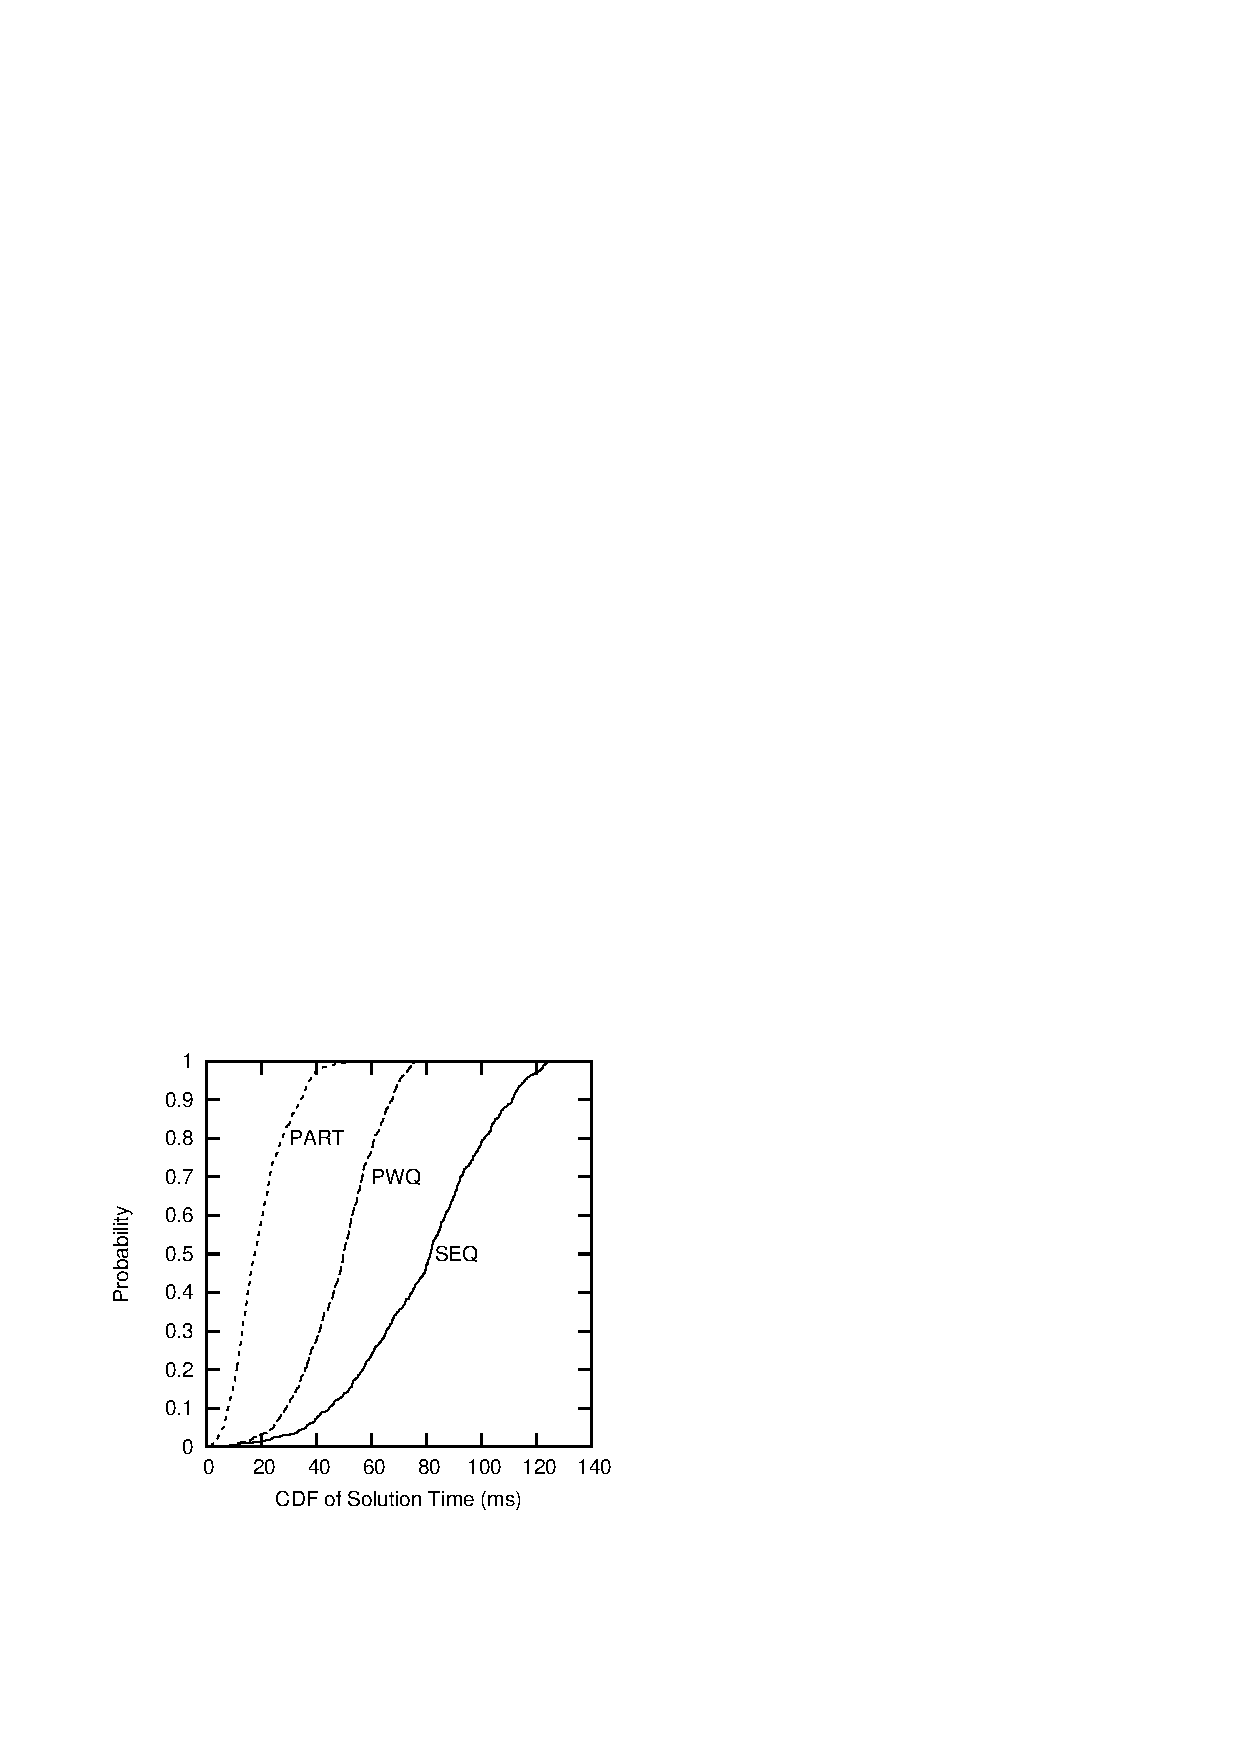
\includegraphics{SMPdesign/500-ms_seq_fg_part-cdf}}
\caption{CDF of Solution Times For SEQ, PWQ, and PART}
\label{fig:SMPdesign:CDF of Solution Times For SEQ, PWQ, and PART}
\end{figure}

성능 테스트는
Figure~\ref{fig:SMPdesign:CDF of Solution Times For SEQ, PWQ, and PART} 에
보여진 것과 같이 심각한 변칙적 결과를 보였습니다.
PART 의 평균 해법 탐색 시간 (17 밀리세컨드) 은 SEQ 의 그것 (79 밀리세컨드) 보다
두개의 쓰레드만 사용함에도 네배 넘게 빨랐습니다.
다음 섹션에서 이 결과를 분석해 봅니다.
\iffalse

Performance testing revealed a surprising anomaly, shown in
Figure~\ref{fig:SMPdesign:CDF of Solution Times For SEQ, PWQ, and PART}.
The median solution time for PART (17 milliseconds)
is more than four times faster than that of SEQ (79 milliseconds),
despite running on only two threads.
The next section analyzes this anomaly.
\fi

\subsection{Performance Comparison I}
\label{sec:SMPdesign:Performance Comparison I}

\begin{figure}[tb]
\centering
\resizebox{2.2in}{!}{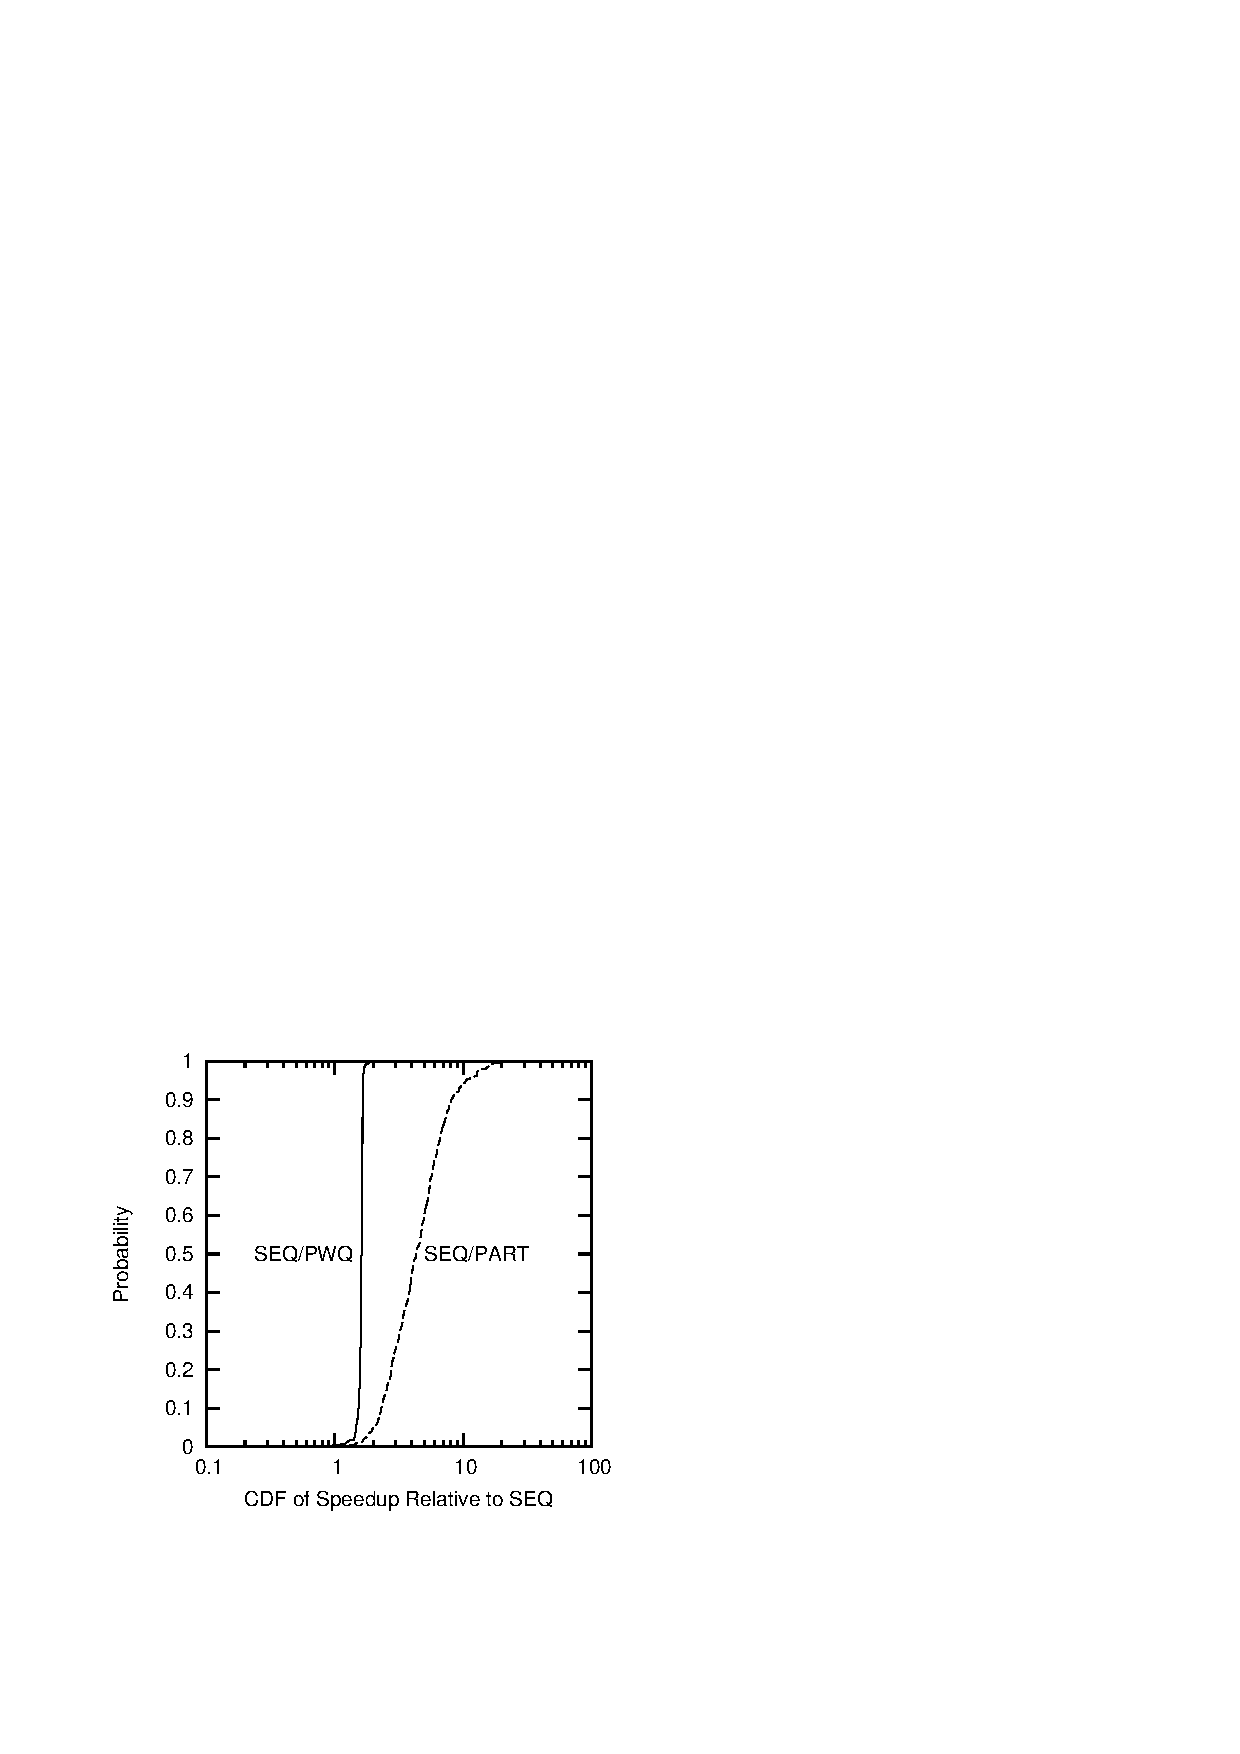
\includegraphics{SMPdesign/500-ms_seqVfg_part-cdf}}
\caption{CDF of SEQ/PWQ and SEQ/PART Solution-Time Ratios}
\label{fig:SMPdesign:CDF of SEQ/PWQ and SEQ/PART Solution-Time Ratios}
\end{figure}

이례적 성능 결과에 대한 첫번째 대응은 버그 유무를 체크하는 것입니다.
이 알고리즘들은 모두 실제로 올바른 해결책을 찾아내고 있습니다만,
Figure~\ref{fig:SMPdesign:CDF of Solution Times For SEQ, PWQ, and PART} 에
나타난 CDF 그림은 독립적인 데이터를 가정하고 있습니다.
이건 올바른 경우가 아닙니다:  이 성능 테스트들은 무작위적으로 미로를 생성하고,
그 미로에 대해 모든 알고리즘들을 돌려보고 있습니다.
따라서 각각의 생성된 미로에 대해 해결책을 찾는데 걸린 시간의 비율의 CDF 를
그려보는게 좀 더 말이 될텐데,
Figure~\ref{fig:SMPdesign:CDF of SEQ/PWQ and SEQ/PART Solution-Time Ratios} 에
그 그림이 그려져 있으며, 여기선 CDF 들의 중복이 훨씬 줄어들었습니다.
쓰레드 두개로 이루어진 40배의 성능 향상은 설명이 필요합니다.
무엇보다, 이것은 단지 파티션으로 쪼갤 수 있음이 쓰레드를 추가하는 것으로 인해
전체 연산 비용의 증가로 이어지지 않음을 의미하는 당혹스러울 정도의 병렬성도
아닙니다.
그 대신, 이것은 \emph{굴욕적인 병렬성} 입니다: 쓰레드를 추가하는 것이 전체 연산
비용을 상당히 줄여줘서 커다란 알고리즘적인 선형적인 성능향상을 초월하는 결과를
이끌어낸 것입니다. 
\iffalse

The first reaction to a performance anomaly is to check for bugs.
Although the algorithms were in fact finding valid solutions, the
plot of CDFs in
Figure~\ref{fig:SMPdesign:CDF of Solution Times For SEQ, PWQ, and PART}
assumes independent data points.
This is not the case:  The performance tests randomly generate a maze,
and then run all solvers on that maze.
It therefore makes sense to plot the CDF of the ratios of
solution times for each generated maze,
as shown in
Figure~\ref{fig:SMPdesign:CDF of SEQ/PWQ and SEQ/PART Solution-Time Ratios},
greatly reducing the CDFs' overlap.
This plot reveals that for some mazes, PART
is more than \emph{forty} times faster than SEQ.
In contrast, PWQ is never more than about
two times faster than SEQ.
A forty-times speedup on two threads demands explanation.
After all, this is not merely embarrassingly parallel, where partitionability
means that adding threads does not increase the overall computational cost.
It is instead \emph{humiliatingly parallel}: Adding threads
significantly reduces the overall computational cost, resulting in
large algorithmic superlinear speedups.
\fi

\begin{figure}[tb]
\centering
\resizebox{1.4in}{!}{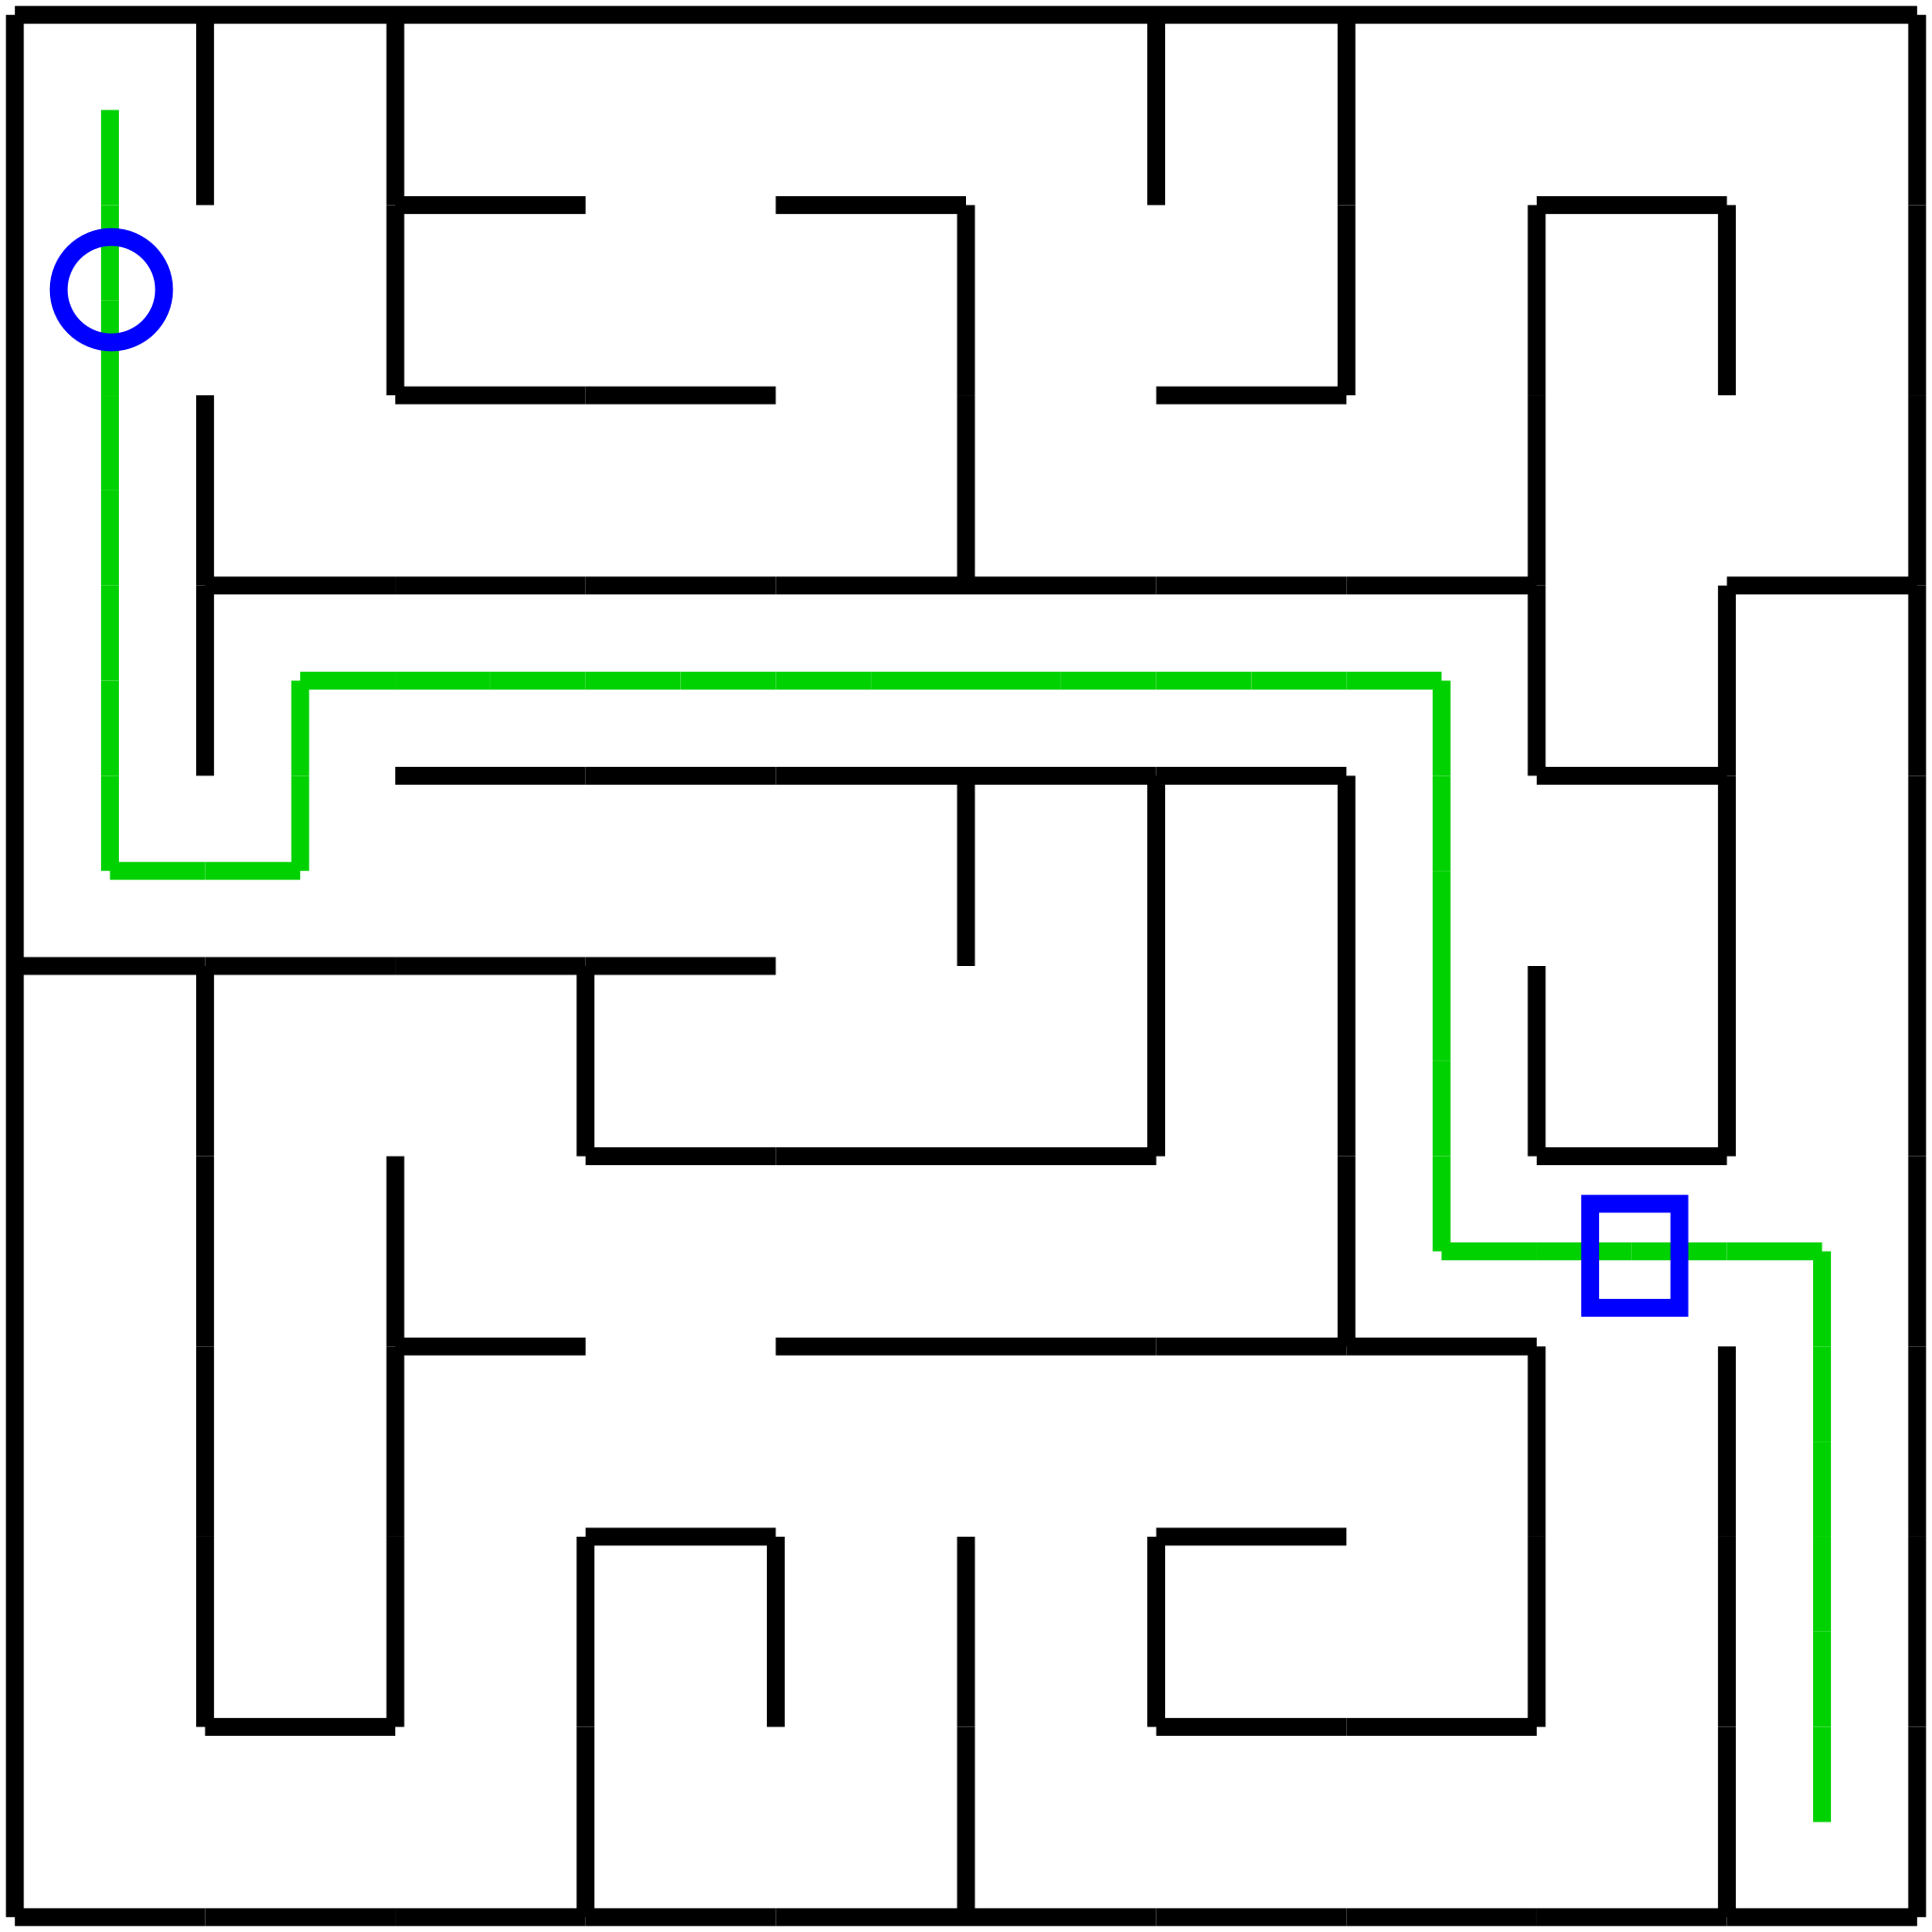
\includegraphics{SMPdesign/maze_in_way10a}}
\caption{Reason for Small Visit Percentages}
\label{fig:SMPdesign:Reason for Small Visit Percentages}
\end{figure}

\begin{figure}[tb]
\centering
\resizebox{2.2in}{!}{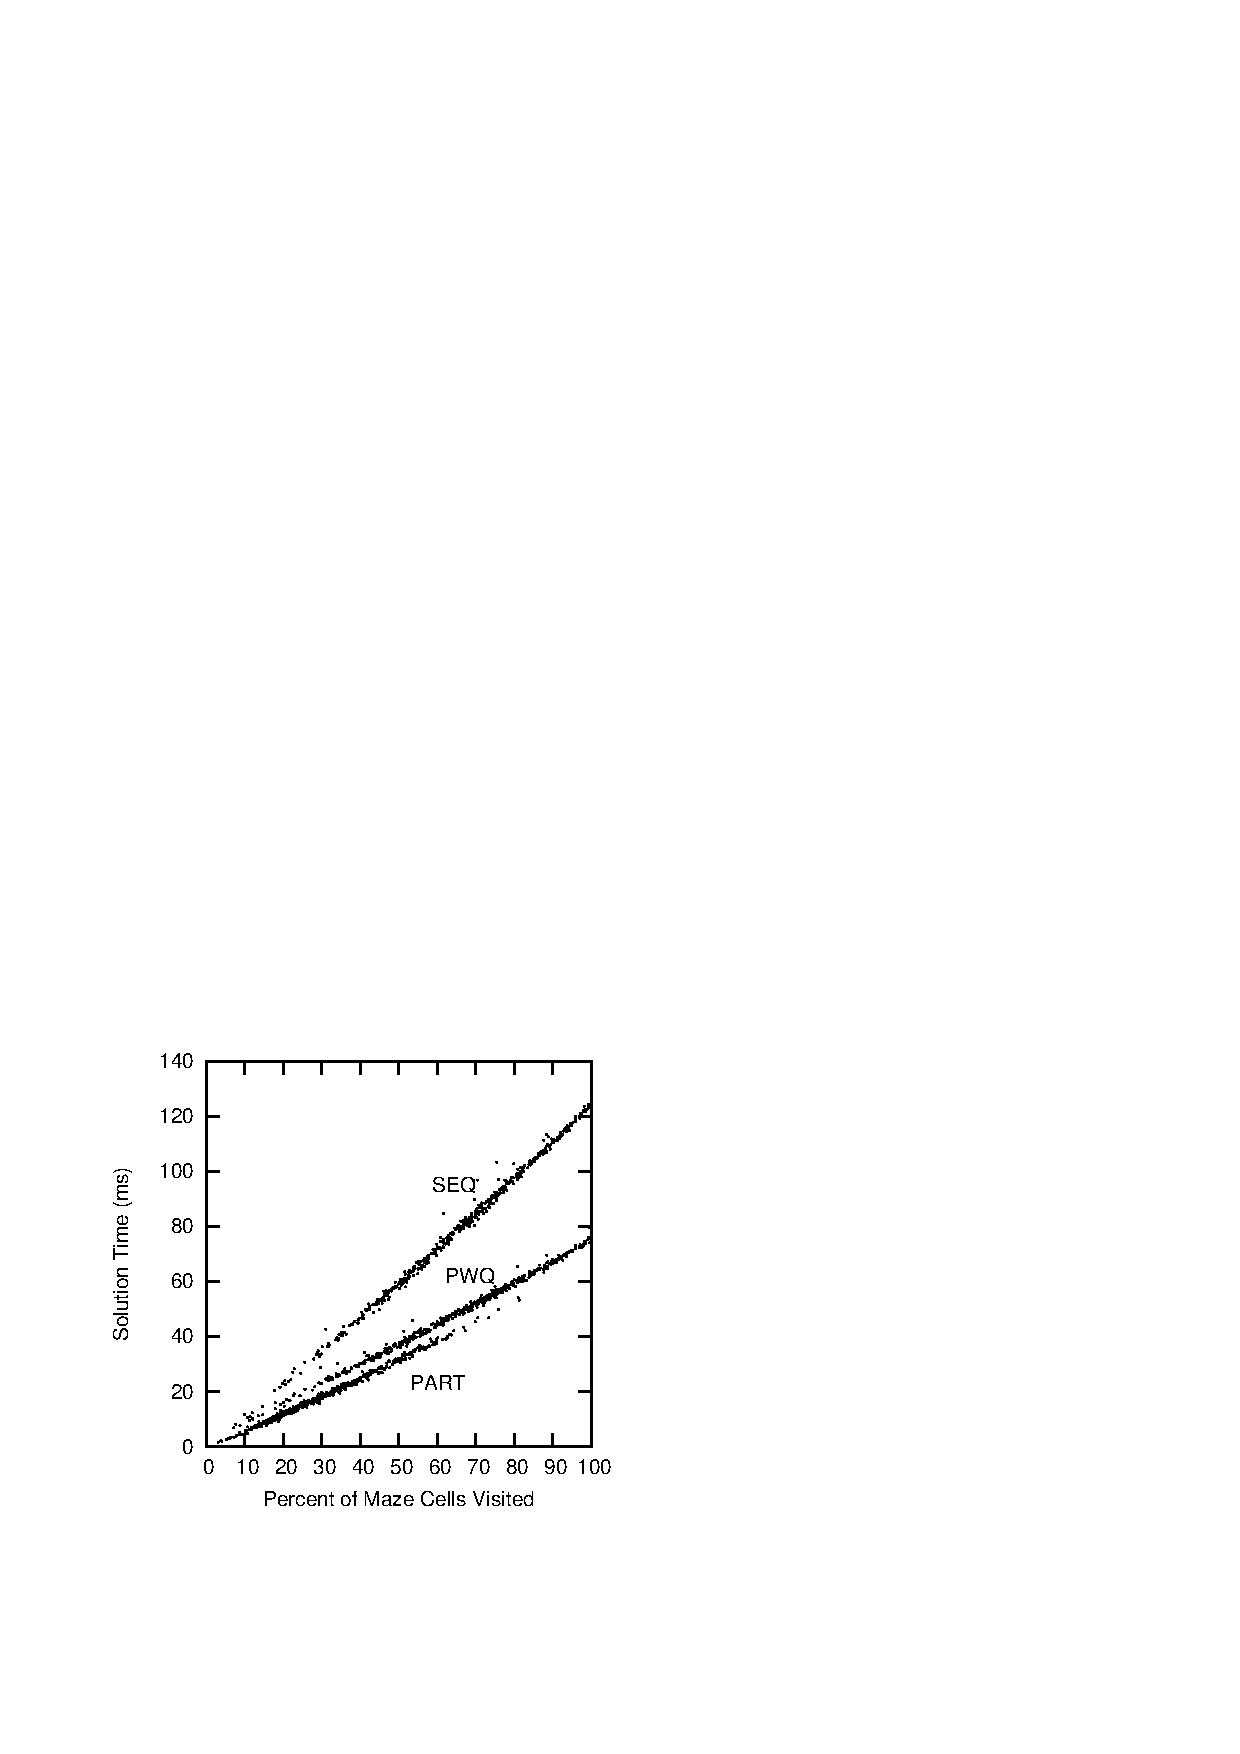
\includegraphics{SMPdesign/500-pctVms_seq_part-sct}}
\caption{Correlation Between Visit Percentage and Solution Time}
\label{fig:SMPdesign:Correlation Between Visit Percentage and Solution Time}
\end{figure}

더 나아가서 들여다본 결과 PART 는 가끔 미로의 셀들 중 2\,\% 미만만을 방문했는데,
SEQ 와 PWQ 는 9\,\% 미만을 방문한 적이 없었습니다.
이런 차이점에 대한 이유는
Figure~\ref{fig:SMPdesign:Reason for Small Visit Percentages} 에 보여져
있습니다.
만약 좌상당부터 시작해서 해결책을 찾는 쓰레드가 원에 도달하면 다른 쓰레드는
미로의 우상단에 도락할 수 없습니다.
비슷하게, 만약 다른 쓰레드가 네모에 도달하면, 첫번째 쓰레드는 미로의 좌하단에
도착할 수 없습니다.
따라서, PART 는 해법이 아닌 셀들로 이루어진 경로 중 더 작은 부분만을 방문하게
될 것입니다.
한마디로, 선형을 초월하는 속도 향상은 쓰레드들이 서로의 길을 만들어 주기
때문입니다.
이는 일하는 쓰레드들이 쓰레드들 각자의 길에서 다른 쓰레드들을 벗어나게 하기
위해 노력해왔던 수십년의 병렬 프로그래밍의 경험에 상당히 반대되는 이야기입니다.
\iffalse

Further investigation showed that
PART sometimes visited fewer than 2\,\% of the maze's cells,
while SEQ and PWQ never visited fewer than about 9\,\%.
The reason for this difference is shown by
Figure~\ref{fig:SMPdesign:Reason for Small Visit Percentages}.
If the thread traversing the solution from the upper left reaches
the circle, the other thread cannot reach
the upper-right portion of the maze.
Similarly, if the other thread reaches the square,
the first thread cannot reach the lower-left
portion of the maze.
Therefore, PART will likely visit a small fraction
of the non-solution-path cells.
In short, the superlinear speedups are due to threads getting in each
others' way.
This is a sharp contrast with decades of experience with
parallel programming, where workers have struggled
to keep threads \emph{out} of each others' way.
\fi

Figure~\ref{fig:SMPdesign:Correlation Between Visit Percentage and Solution Time}
는 세개의 모든 방법들에 대해 방문된 셀들의 수와 해결책 탐색에 걸리는 시간
사이의 강한 상관관계를 확실히 보여주고 있습니다.
PART 의 그림의 경사도는 SEQ 의 그것에 비해 작은데, 이것이 PART 의 쓰레드들이
SEQ 의 단일 쓰레드에 비해 미로의 주어진 부분을 더 빠르게 방문할 것임을 이야기
합니다.
PART 의 그림은 또한 작은 방문 퍼센티지에 몰려 있는데, 이는 PART 가 더 적은 일을
하게 되며, 따라서 관측된 굴욕적인 병렬성을 보이게 되는 것입니다.
\iffalse

Figure~\ref{fig:SMPdesign:Correlation Between Visit Percentage and Solution Time}
confirms a strong correlation between cells visited and solution time
for all three methods.
The slope of PART's scatterplot is smaller than that of SEQ,
indicating that PART's pair of threads visits a given fraction
of the maze faster than can SEQ's single thread.
PART's scatterplot is also weighted toward small visit
percentages, confirming that PART does less total work, hence
the observed humiliating parallelism.
\fi

\begin{figure}[tb]
\centering
\resizebox{1.4in}{!}{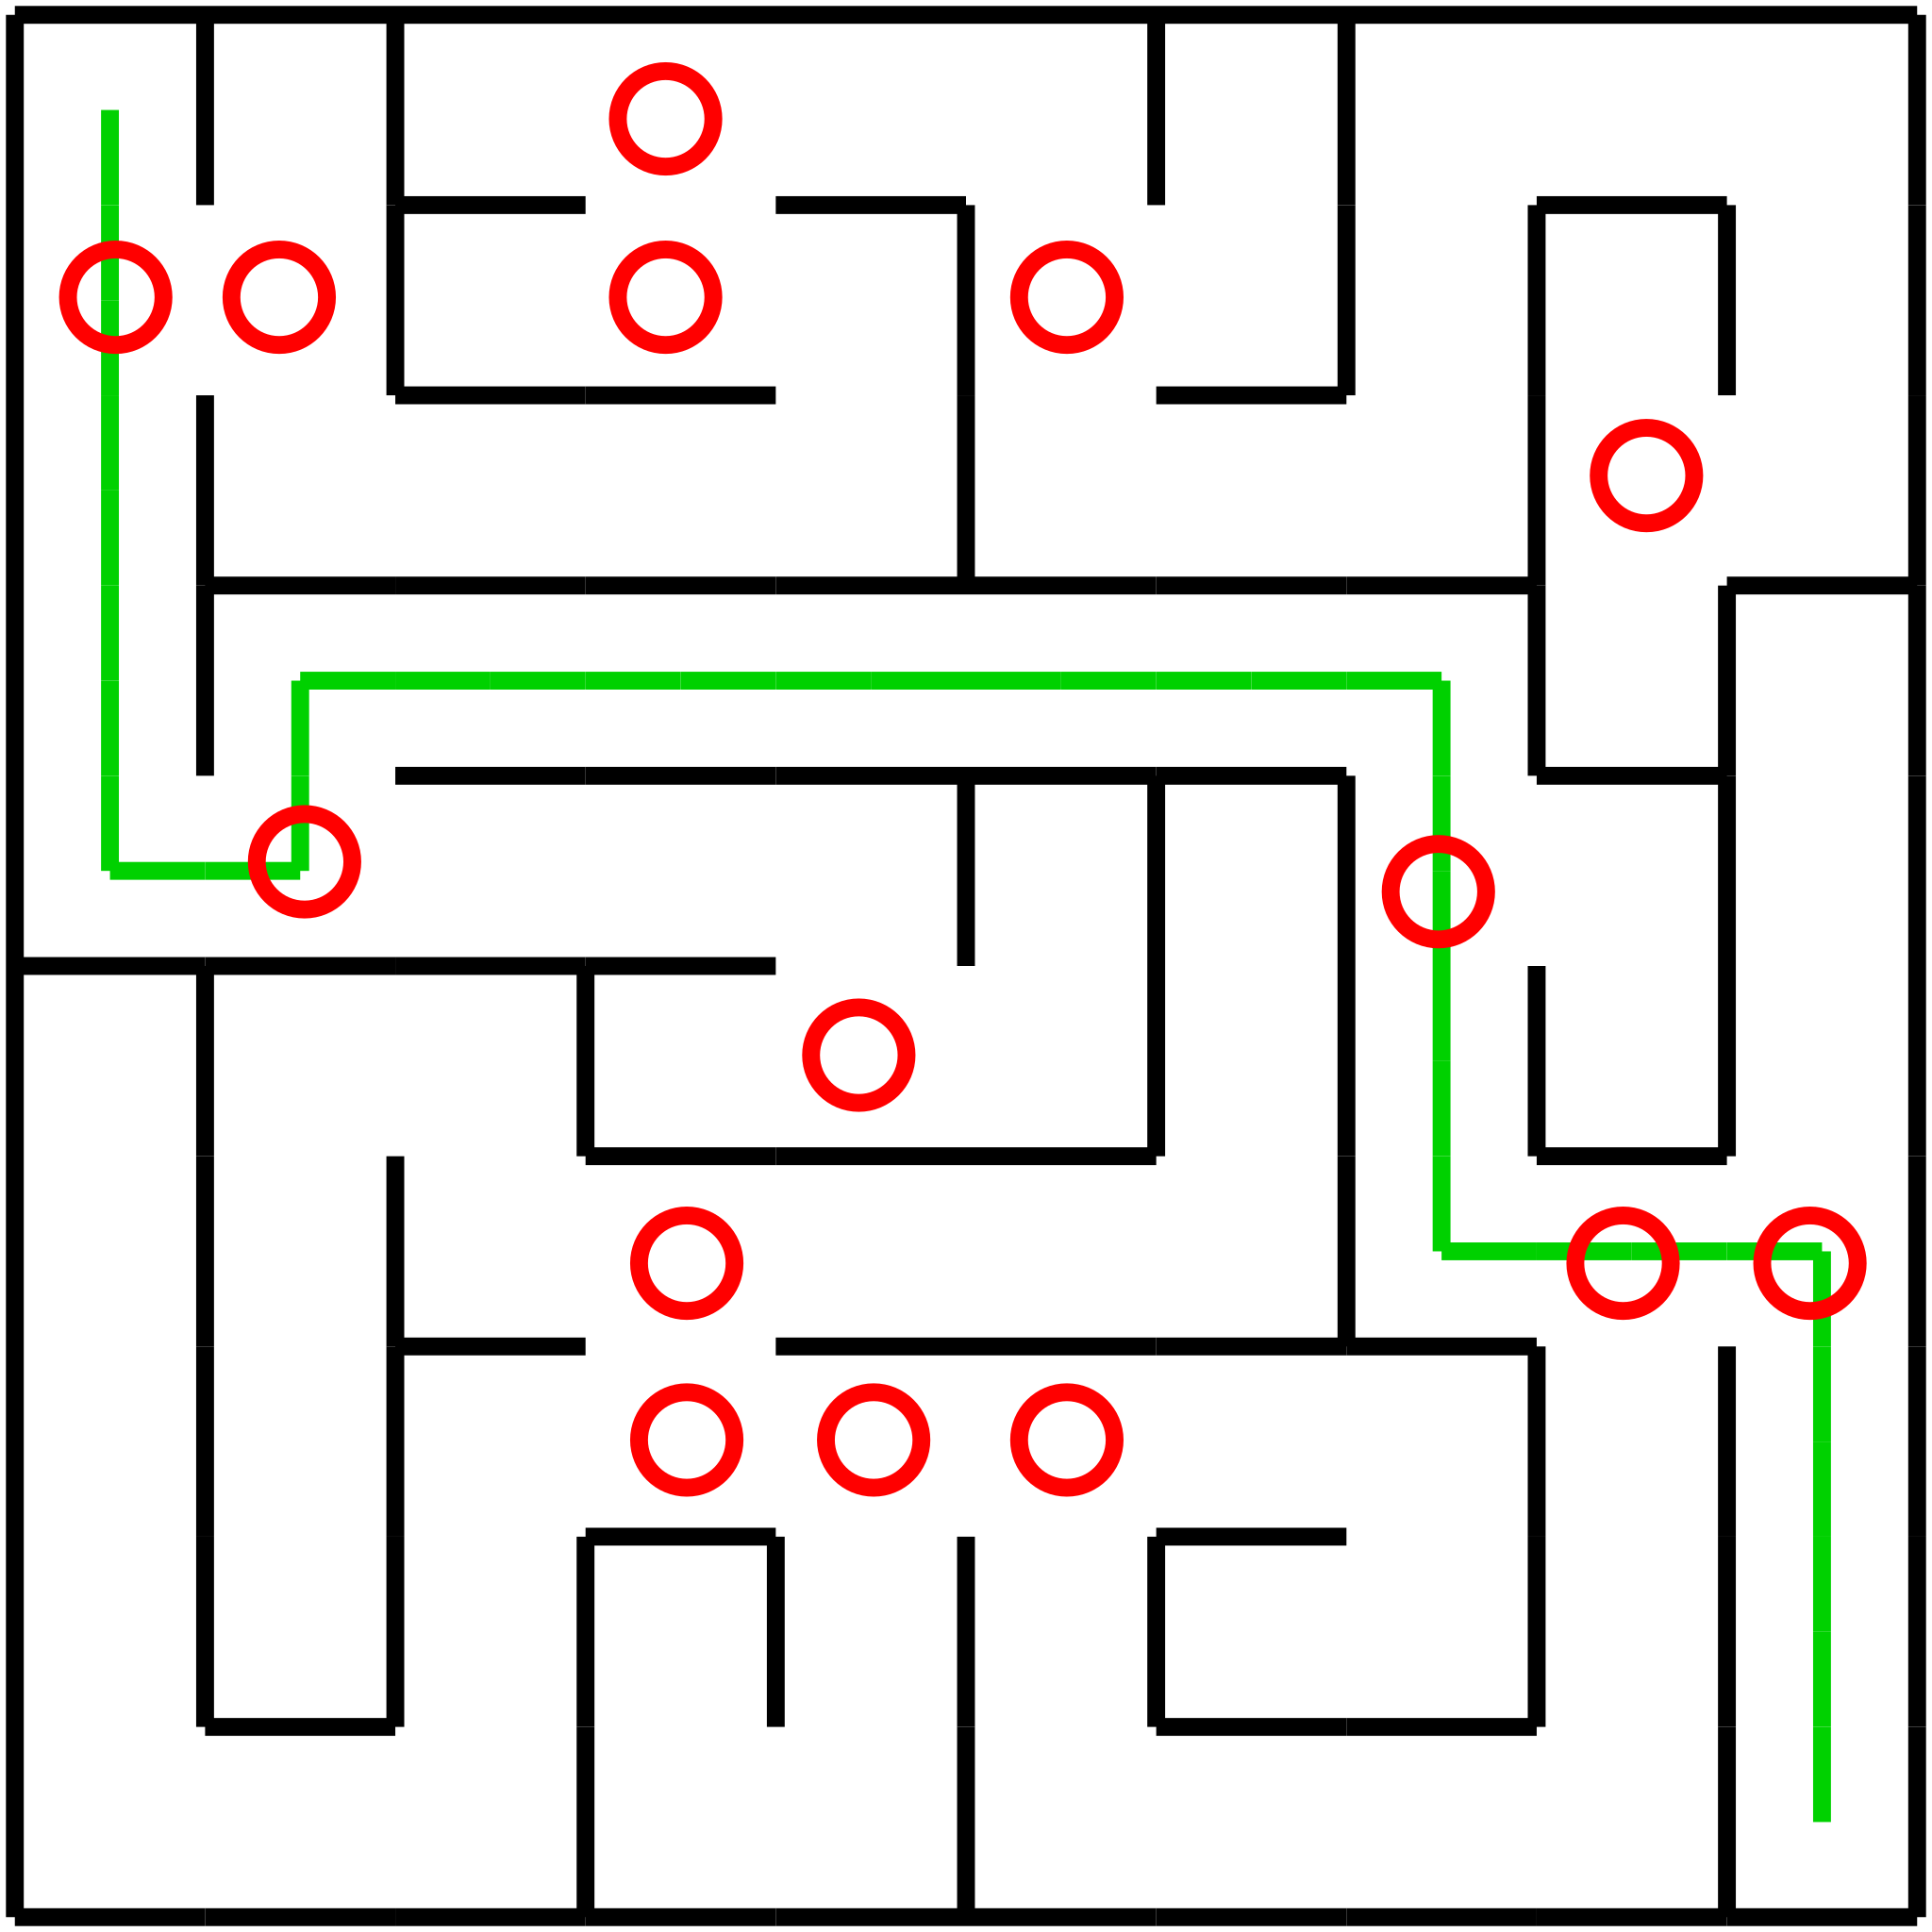
\includegraphics{SMPdesign/maze_PWQ_vs_PART}}
\caption{PWQ Potential Contention Points}
\label{fig:SMPdesign:PWQ Potential Contention Points}
\end{figure}

PWQ 에 의해 방문되는 셀들로 이루어진 부분들은 SEQ 의 그것과 유사합니다.
또한, PWQ 의 해결책 탐색에 걸리는 시간은 동일한 방문 부분들에도 불구하고 PART
의 그것에 비해 훨씬 큽니다.
이에 대한 이유가 Figure~\ref{fig:SMPdesign:PWQ Potential Contention Points} 에
그려져 있는데, 이 그림에는 두개 이상의 이웃을 가지고 있는 셀마다 붉은 원을
그려두었습니다.
그러한 각각의 셀은 PWQ 에서 경쟁 상황을 초래할 수 있는데, 한 쓰레드는 들어갈 수
있지만 두 쓰레드들이 나갈 수 있기 때문에, 이 챕터의 앞부분에서 설명했듯이
성능을 악화시킬 수 있기 때문입니다.
반면에 PART 는 그런 경쟁상황을 한번만 일으키는데, 해법이 찾아졌을 때입니다.
물론, SEQ 는 경쟁상황은 일으키지 않습니다.
\iffalse

The fraction of cells visited by PWQ is similar to that of SEQ.
In addition, PWQ's solution time is greater than that of PART,
even for equal visit fractions.
The reason for this is shown in
Figure~\ref{fig:SMPdesign:PWQ Potential Contention Points}, which has a red
circle on each cell with more than two neighbors.
Each such cell can result in contention in PWQ, because
one thread can enter but two threads can exit, which hurts
performance, as noted earlier in this chapter.
In contrast, PART can incur such contention but once, namely
when the solution is located.
Of course, SEQ never contends.
\fi

\begin{figure}[tb]
\centering
\resizebox{2.2in}{!}{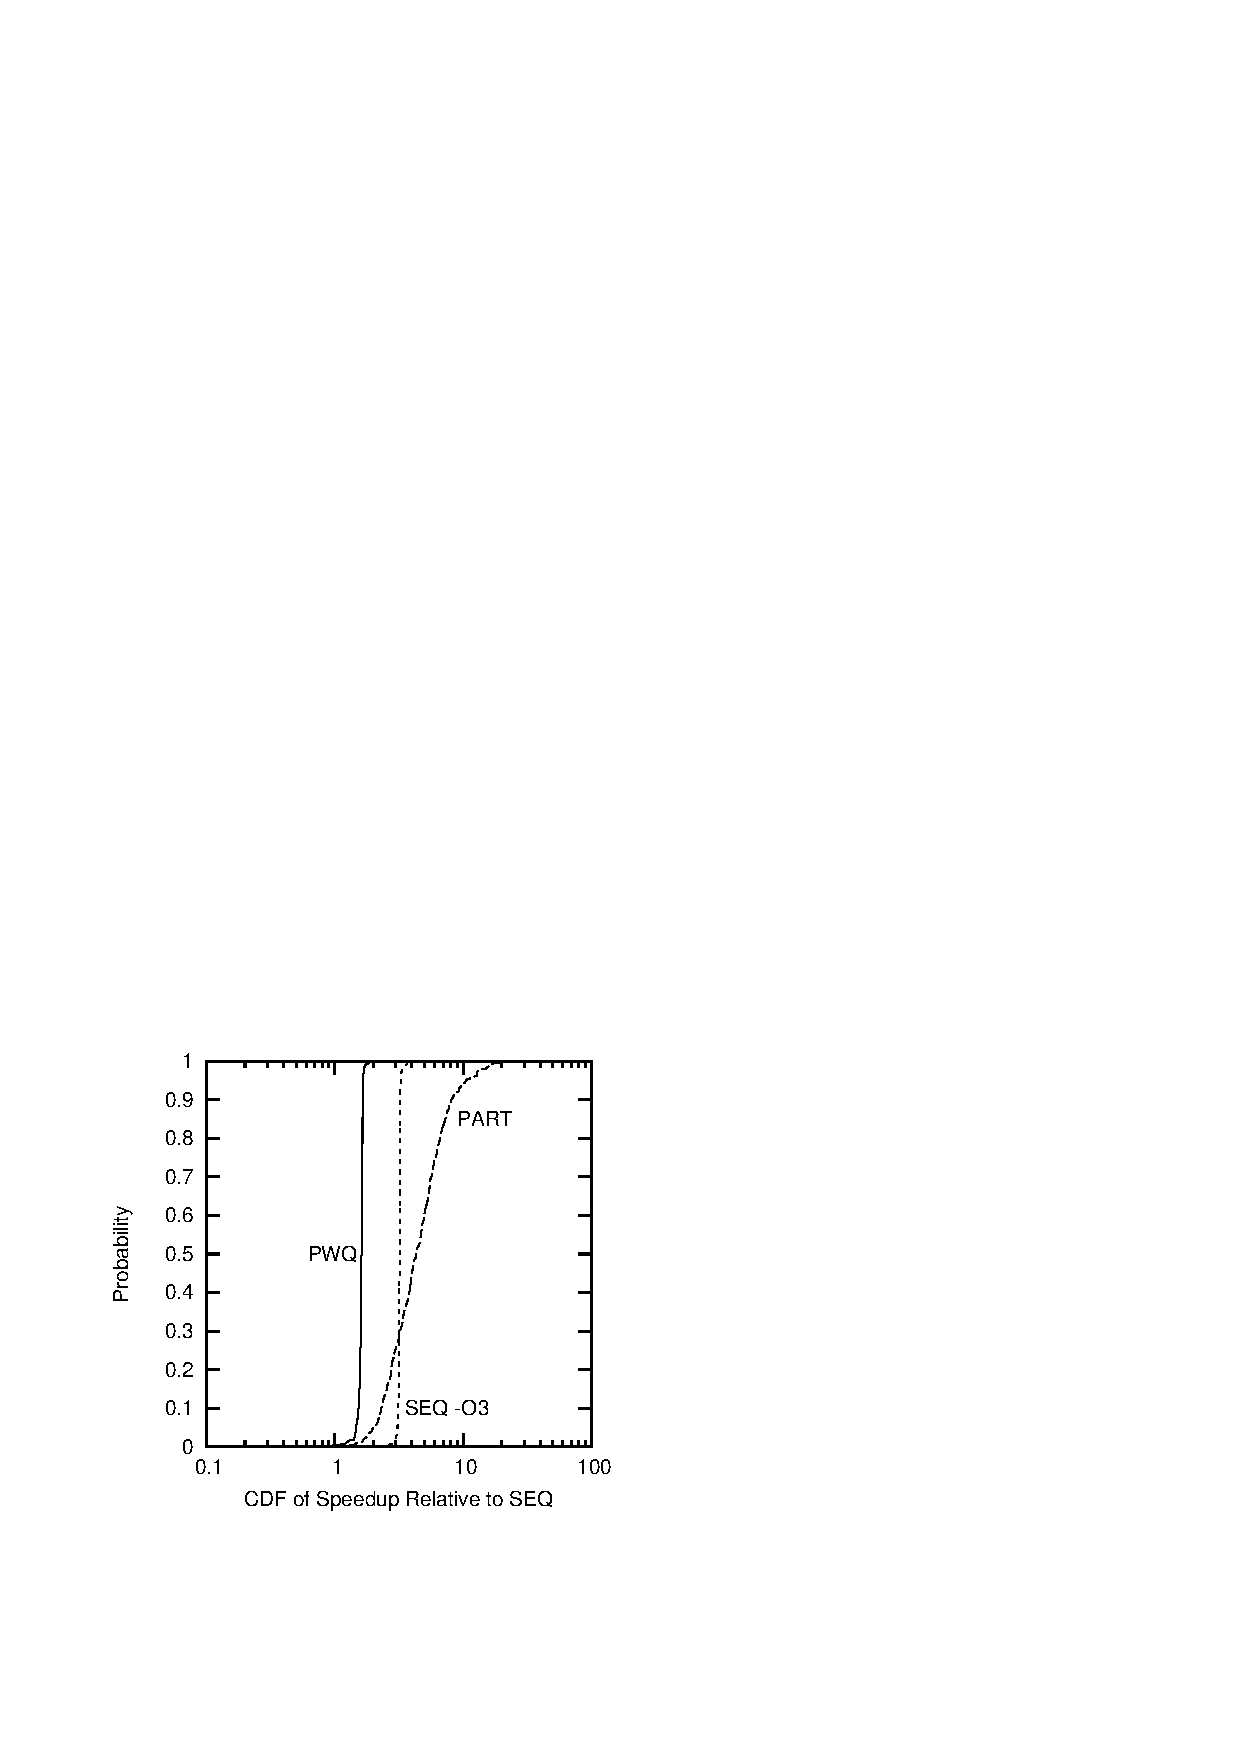
\includegraphics{SMPdesign/500-ms_seqVfg_part_seqO3-cdf}}
\caption{Effect of Compiler Optimization (-O3)}
\label{fig:SMPdesign:Effect of Compiler Optimization (-O3)}
\end{figure}

PART 의 성능 향상이 인상적이긴 하지만, 순차적인 최적화를 게을리 하지는 않아야
합니다.
Figure~\ref{fig:SMPdesign:Effect of Compiler Optimization (-O3)} 는 SEQ 가 -O3
옵션을 가지고 컴파일 되었을 때에는 최적화 되지 않은 PWQ 보다 두배 정도나
빠르고, 최적화 되지 않은 PART 의 성능에 근접합니다.
세개의 알고리즘을 모두 -O3 옵션을 주고 컴파일한 결과는 (더 빠르긴 하지만)
Figure~\ref{fig:SMPdesign:CDF of SEQ/PWQ and SEQ/PART Solution-Time Ratios} 에
보여진 그것들과 비슷한 양상을 보입니다만, PWQ 가 SEQ 에 비해 속도향상을 거의
보이지 않는다는 예외를 갖는데, 이는
Amdahl 의 법칙~\cite{GeneAmdahl1967AmdahlsLaw} 에 의함입니다.
하지만, 최적화 되지 않은 SEQ 에 비해 두배의 속도를 갖는게 목표라면, 컴파일러
최적화는 상당히 매력적인 방법이라 할 수 있겠습니다.
\iffalse

Although PART's speedup is impressive, we should not neglect sequential
optimizations.
Figure~\ref{fig:SMPdesign:Effect of Compiler Optimization (-O3)} shows that
SEQ, when compiled with -O3, is about twice as fast
as unoptimized PWQ, approaching the performance of unoptimized PART.
Compiling all three algorithms with -O3 gives results similar to
(albeit faster than) those shown in
Figure~\ref{fig:SMPdesign:CDF of SEQ/PWQ and SEQ/PART Solution-Time Ratios},
except that PWQ provides almost no speedup compared
to SEQ, in keeping with Amdahl's Law~\cite{GeneAmdahl1967AmdahlsLaw}.
However, if the goal is to double performance compared to unoptimized
SEQ, as opposed to achieving optimality, compiler
optimizations are quite attractive.
\fi

캐시 정렬과 패딩이 종종 거짓 공유 (false sharing) 을 줄여서 성능을 개선시키곤
합니다.
하지만, 이 미로 해법 알고리즘들에 있어서는, 미로 셀 배열에 정렬과 패딩을
적용하는 것은 1000x1000 미로에 대해 42\,\% 까지 성능을 \emph{떨어뜨립니다}.
캐시 로컬리티는 거짓 공유를 없애는 것보다 더 중요한데, 특히나 큰 미로에선 더욱
그러합니다.
작은 20x20 이나 50x50 미로에서라면, 정렬과 패딩이 PART 에 대해 성능을 40\,\% 까지
향상시킬 수 있습니다만 이런 작은 크기의 미로에 대해서는 PART 가 쓰레드를
생성하고 소멸시키는데 드는 오버헤드를 상쇄시키기에 충분한 시간을 갖지 못하기에
SEQ 가 더 좋은 성능을 보입니다.

정리하자면, 파티셔닝을 사용한 병렬 미로 해결책은 알고리즘적으로 선형을 초월한
속도향상의 하나의 재미있는 예입니다.
만약 ``알고리즘적으로 선형을 초월한 속도 향상'' 이 인지 부조화를 일으킨다면,
다음 섹션으로 넘어가 보시기 바랍니다.
\iffalse

Cache alignment and padding often improves performance by reducing
false sharing.
However, for these maze-solution algorithms, aligning and padding the
maze-cell array \emph{degrades} performance by up to 42\,\% for 1000x1000 mazes.
Cache locality is more important than avoiding
false sharing, especially for large mazes.
For smaller 20-by-20 or 50-by-50 mazes, aligning and padding can produce
up to a 40\,\% performance improvement for PART,
but for these small sizes, SEQ performs better anyway because there
is insufficient time for PART to make up for the overhead of
thread creation and destruction.

In short, the partitioned parallel maze solver is an interesting example
of an algorithmic superlinear speedup.
If ``algorithmic superlinear speedup'' causes cognitive dissonance,
please proceed to the next section.
\fi

\subsection{Alternative Sequential Maze Solver}
\label{sec:SMPdesign:Alternative Sequential Maze Solver}

\begin{figure}[tb]
\centering
\resizebox{2.2in}{!}{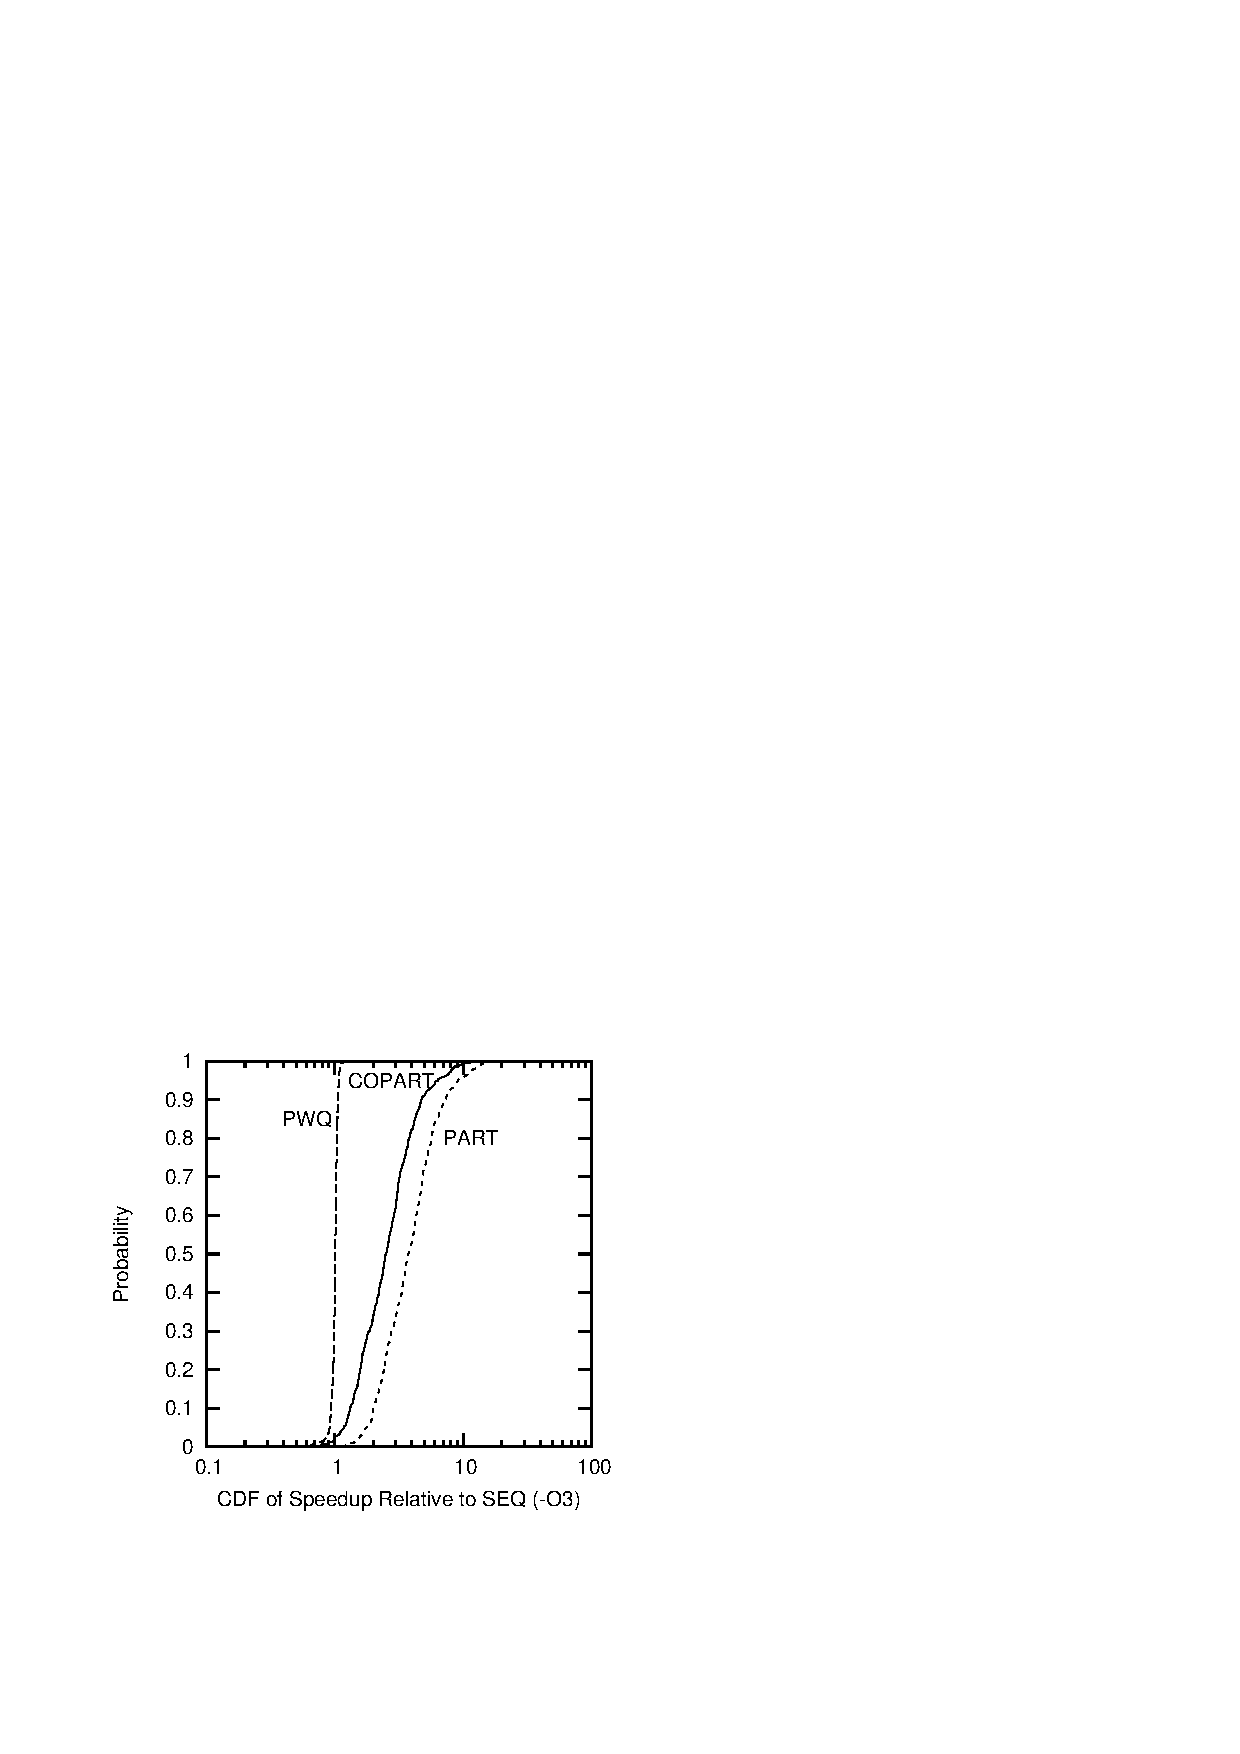
\includegraphics{SMPdesign/500-ms_seqO3V2seqO3_fgO3_partO3-cdf}}
\caption{Partitioned Coroutines}
\label{fig:SMPdesign:Partitioned Coroutines}
\end{figure}

알고리즘적으로 선형을 초월한 속도 향상의 존재는 코루틴 (co-routine) 을 통한
병렬성 모의실험을 제시하는데, 예를 들어, Listing~\ref{lst:SMPdesign:Partitioned
Parallel Solver Pseudocode} 의 do-while 루프의 각 패스에서 수동으로 컨텍스트
스위칭을 해보는 겁니다.
이 컨텍스트 스위칭은 직접적인데 이 컨텍스트는 변수들 \co{c} 와 \co{vi} 로만
구성되어 있기 때문입니다: 이 효과를 낼 수 있는 많은 방법들 중, 이 방법이
컨텍스트 스위칭 오버헤드와 방문 퍼센티지 사이의 좋은 트레이드오프입니다.
Figure~\ref{fig:SMPdesign:Partitioned Coroutines} 에서 볼 수 있듯이 이 코루틴
알고리즘 (COPART) 은 상당히 효과적으로, 한 쓰레드에서의 성능이 두 쓰레드를
사용한 PART 의 30\,\% 입니다(\co{maze_2seq.c}).
\iffalse

The presence of algorithmic superlinear speedups suggests simulating
parallelism via co-routines, for example, manually switching context
between threads on each pass through the main do-while loop in
Listing~\ref{lst:SMPdesign:Partitioned Parallel Solver Pseudocode}.
This context switching is straightforward because the context
consists only of the variables \co{c} and \co{vi}: Of the numerous
ways to achieve the effect, this is a good tradeoff between
context-switch overhead and visit percentage.
As can be seen in
Figure~\ref{fig:SMPdesign:Partitioned Coroutines},
this coroutine algorithm (COPART) is quite effective, with the performance
on one thread being within about 30\,\% of PART on two threads
(\path{maze_2seq.c}).
\fi

\subsection{Performance Comparison II}
\label{sec:SMPdesign:Performance Comparison II}

\begin{figure}[tb]
\centering
\resizebox{2.2in}{!}{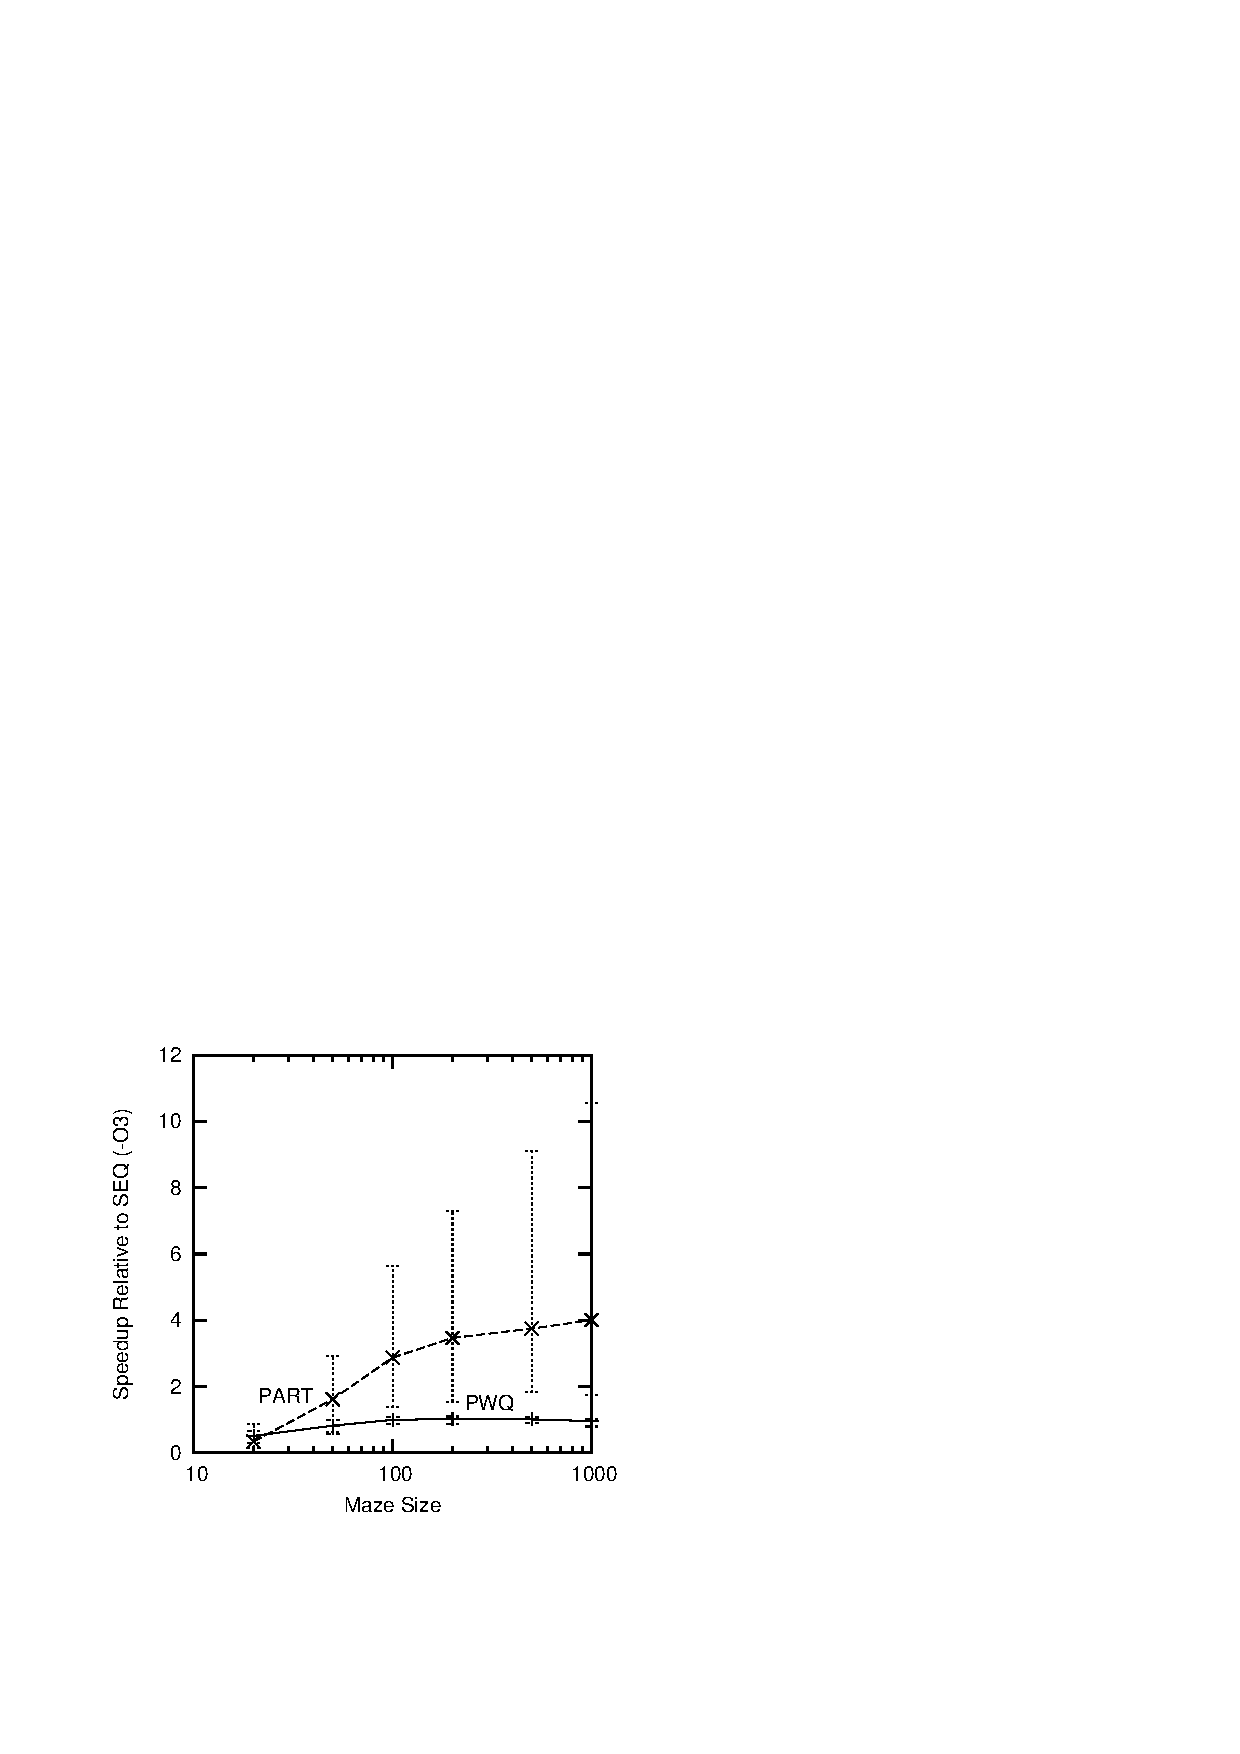
\includegraphics{SMPdesign/500-ms_seqO3VfgO3_partO3-median}}
\caption{Varying Maze Size vs. SEQ}
\label{fig:SMPdesign:Varying Maze Size vs. SEQ}
\end{figure}

\begin{figure}[tb]
\centering
\resizebox{2.2in}{!}{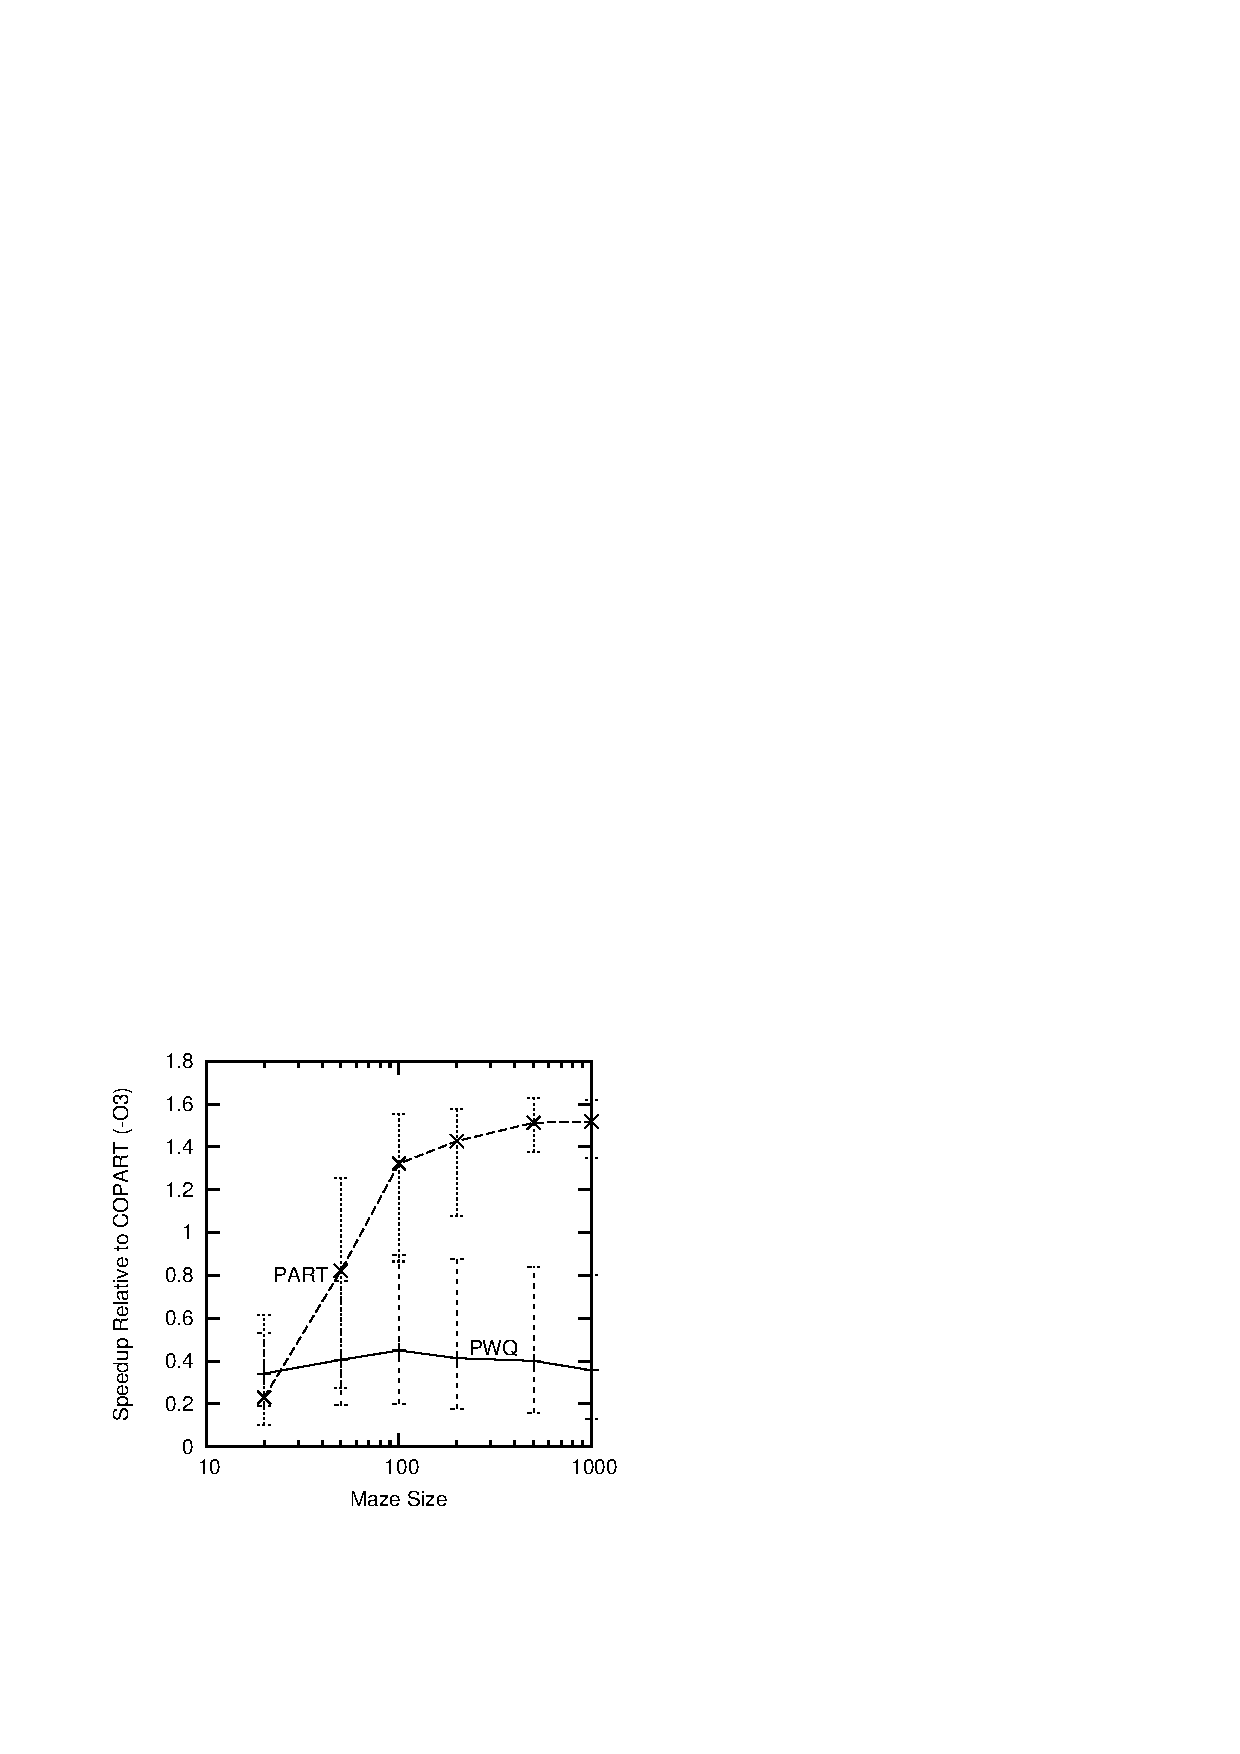
\includegraphics{SMPdesign/500-ms_2seqO3VfgO3_partO3-median}}
\caption{Varying Maze Size vs. COPART}
\label{fig:SMPdesign:Varying Maze Size vs. COPART}
\end{figure}

Figures~\ref{fig:SMPdesign:Varying Maze Size vs. SEQ}
와~\ref{fig:SMPdesign:Varying Maze Size vs. COPART} 는 미로의 크기의 변화에
따른 효과를 두개의 쓰레드로 동작하는 PWQ 와 PART 를 SEQ 또는 COPART 와 각각
비교해 90\,\% 의 정확성 에러 막대와 함께 보여주고 있습니다.
PART 는 100행 100열 이상 크기의 미로들에서 SEQ 에 비해 선형성을 초월한 확장성을
보이고 COPART 에 비해서는 적당한 확장성을 보입니다.
에너지 소모가 높은 주파수에서는 대략 주파수의 제곱 정도로 증가한다는
가정~\cite{TrevorMudge2000Power} 에 기반해서 보면 두 쓰레드를 사용해서 1.4 배의
확장성을 갖는 것은 단일 쓰레드가 같은 해법 탐색 시간을 필요로 할 때 소모하는
에너지와 동일하므로 PART 는 COPART 에 비교했을때 대략 200행 200열 크기 미로에서
이론적인 에너지 효율성 손익분기를 넘어섭니다.
반면, PWQ 는 SEQ 에 대해서도 COPART 에 대해서도 빈약한 확장성을 보이는데, 이는
최적화가 적용되었을 때 이야기입니다: Figure~\ref{fig:SMPdesign:Varying Maze
Size vs. SEQ}
와~\ref{fig:SMPdesign:Varying Maze Size vs. COPART} 는 -O3 옵션을 사용해
만들어졌습니다.
\iffalse

Figures~\ref{fig:SMPdesign:Varying Maze Size vs. SEQ}
and~\ref{fig:SMPdesign:Varying Maze Size vs. COPART}
show the effects of varying maze size, comparing both PWQ and PART
running on two threads
against either SEQ or COPART, respectively, with 90\=/percent\-/confidence
error bars.
PART shows superlinear scalability against SEQ and modest scalability
against COPART for 100-by-100 and larger mazes.
PART exceeds theoretical energy-efficiency breakeven against COPART at roughly
the 200-by-200 maze size, given that power consumption rises as roughly
the square of the frequency for high frequencies~\cite{TrevorMudge2000Power},
so that 1.4x scaling on two threads consumes the same energy
as a single thread at equal solution speeds.
In contrast, PWQ shows poor scalability against both SEQ and COPART
unless unoptimized: Figures~\ref{fig:SMPdesign:Varying Maze Size vs. SEQ} 
and~\ref{fig:SMPdesign:Varying Maze Size vs. COPART}
were generated using -O3.
\fi

\begin{figure}[tb]
\centering
\resizebox{2.2in}{!}{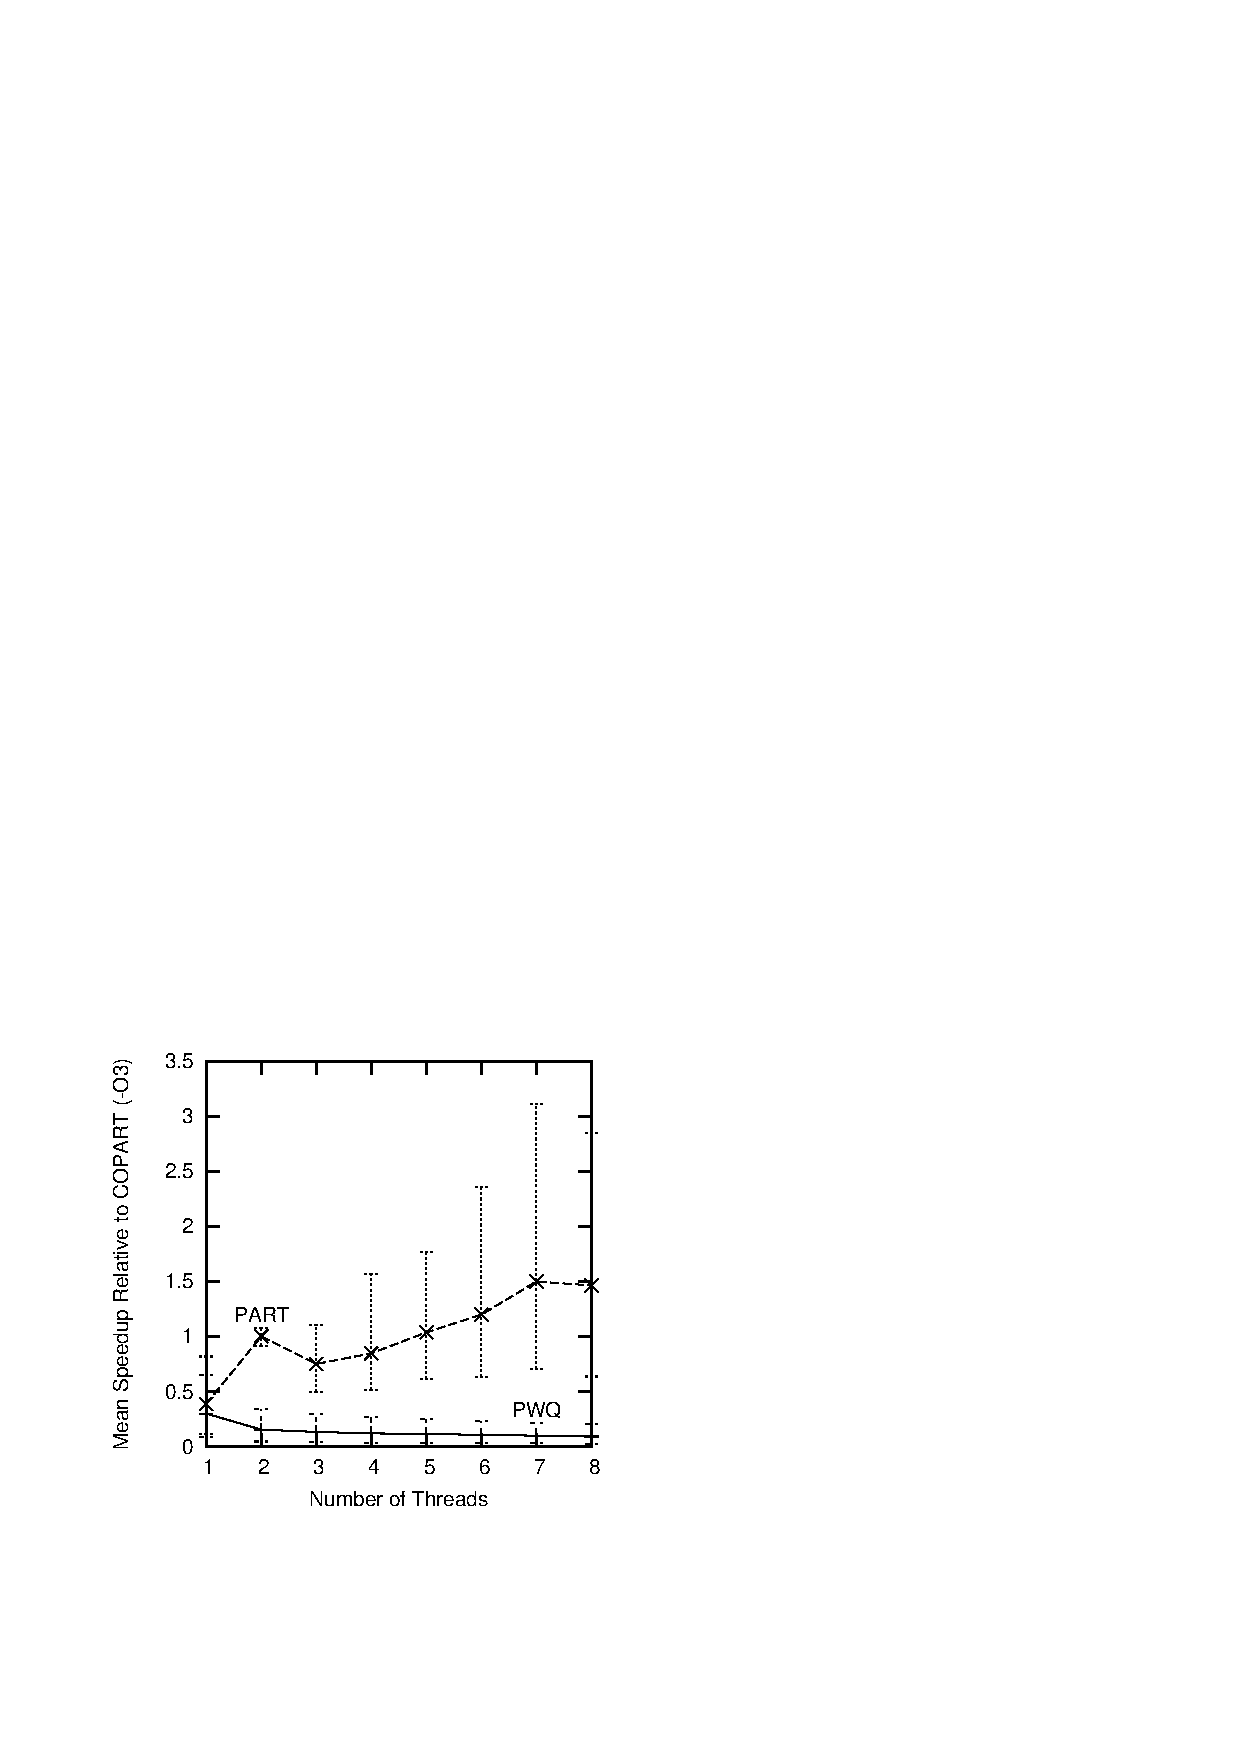
\includegraphics{SMPdesign/1000-ms_2seqO3VfgO3_partO3-mean}}
\caption{Mean Speedup vs. Number of Threads, 1000x1000 Maze}
\label{fig:SMPdesign:Mean Speedup vs. Number of Threads, 1000x1000 Maze}
\end{figure}

Figure~\ref{fig:SMPdesign:Mean Speedup vs. Number of Threads, 1000x1000 Maze}
는 PWQ 와 PART 의 성능을 COPART 에 비교해서 보여주고 있습니다.
두개가 넘는 쓰레드들을 사용해 동작하는 PART 의 경우, 추가된 쓰레드들은 미로의
시작점과 끝점 사이를 대각선으로 동일한 거리로 나뉘어진 위치에서부터 경로 탐색을
시작합니다.
두개가 넘는 쓰레드들을 사용해 동작하는 PART 의 이른 종료를 알아채기 위해서는
간략화된 링크 상태 라우팅~\cite{BERT-87} 이 사용되었습니다 (해법은 한 쓰레드가
시작점과 끝점과 연결되면 찾아진 것으로 표시됩니다).
PWQ 는 상당히 나쁜 성능 결과를 보입니다만, PART 는 두개 쓰레드에서, 그리고
다섯개 쓰레드에서 한번 더 손익분기에 도달하는데 다섯개 쓰레드를 넘어서고부터는
적당한 속도향상을 이루어냅니다.
이론적인 에너지 효율성 손익분기는 7개와 8개 쓰레드들에 대해서는 90\,\% 신뢰구간
안에 있습니다.
두개 쓰레드에서 성능이 뾰족하게 솟아오르는 이유는 (1) 두개 쓰레드의 경우의 덜
복잡한 해법 탐색 종료 파악 과정과 (2) 세번째와 그 뒤의 쓰레드들이 유용한 진전을
만들 확률이 좀 더 낮은 편이라는 사실입니다: 오직 처음의 두 쓰레드만이 해법의
경로에 직결됨이 보장됩니다.
Figure~\ref{fig:SMPdesign:Varying Maze Size vs. COPART} 에 비해 비교적
실망스러운 이 성능 결과는 2.66GHz 로 동작하는 더 크고 오래된
Xeon\textsuperscript\textregistered 에 사용되는 덜 밀접하게 융합된 하드웨어의
탓입니다.
\iffalse

Figure~\ref{fig:SMPdesign:Mean Speedup vs. Number of Threads, 1000x1000 Maze}
shows the performance of PWQ and PART relative to COPART.
For PART runs with more than two threads, the additional threads were
started evenly spaced along the diagonal connecting the starting and
ending cells.
Simplified link-state routing~\cite{BERT-87} was used to
detect early termination on PART runs with more than two threads
(the solution is flagged when
a thread is connected to both beginning and end).
PWQ performs quite poorly, but
PART hits breakeven at two threads and again at five threads, achieving
modest speedups beyond five threads.
Theoretical energy efficiency breakeven is within the 90\=/percent\-/confidence
interval for seven and eight threads.
The reasons for the peak at two threads are (1) the lower complexity
of termination detection in the two-thread case and (2) the fact that
there is a lower probability of the third and subsequent threads making
useful forward progress: Only the first two threads are guaranteed to start on
the solution line.
This disappointing performance compared to results in
Figure~\ref{fig:SMPdesign:Varying Maze Size vs. COPART}
is due to the less-tightly integrated hardware available in the
larger and older Xeon\mytextregistered\
system running at 2.66\,GHz.
\fi

\subsection{Future Directions and Conclusions}
\label{sec:SMPdesign:Future Directions and Conclusions}

너무 많은 해야할 일들이 남아있습니다.
첫째로, 이 섹션은 사람이 미로 해법 탐색 사용하는 방법 가운데 하나의 방법만을
적용해 보았습니다.
이외의 방법으로는 미로의 일부를 제거하기 위해 벽을 따라가는 방법과 이전에
탐색한 경로의 위치에 기반해서 내부 시작 지점을 고르는 방법 등이 있습니다.
둘째로, 시작지점과 끝지점의 다른 선택은 다른 알고리즘에 좀 더 효과적일 수
있습니다.
셋째로, PART 알고리즘의 첫번째 적용했던 방법인 두개 쓰레드 사용이 직선적이긴
하지만, 다른 여분의 쓰레드들을 사용하기 위한 방법들이 여럿 있습니다.
최적의 쓰레드 사용은 시작지점과 끝지점에도 의존적일 것입니다.
넷째로, 해결이 불가능한 미로들과 순환적인 미로들에 대한 연구는 재미있는 결과를
내놓을 수 있을 것입니다.
다섯째로, 가벼운 C++11 어토믹 오퍼레이션들은 성능을 개선시킬 수도 있습니다.
여섯째로, 3차원 미로 (또는 그보다도 높은 차원의 미로들) 의 속도 향상을 비교해
보는 것도 재미있을 것입니다.
마지막으로, 미로의 경우, 굴욕적 병렬성은 코루틴들을 사용한 보다 효과적인 순차적
구현을 의미했습니다.
굴욕적 병렬성 알고리즘은 항상 더 효과적인 순차적 구현을 이끌게 될까요, 아니면
코루틴 컨텍스트 스위치 오버헤드가 속도향상을 압도해버리는 고유의 굴욕적 병렬성
알고리즘이 존재할까요?
\iffalse

Much future work remains.
First, this section applied only one technique used by human maze solvers.
Others include following walls to exclude portions of the maze
and choosing internal starting points based on the
locations of previously traversed paths.
Second, different choices of
starting and ending points might favor different algorithms.
Third, although placement of the PART algorithm's
first two threads is straightforward, there are any number of
placement schemes for the remaining threads.
Optimal placement might well depend on the starting and ending points.
Fourth, study of unsolvable mazes and cyclic mazes
is likely to produce interesting results.
Fifth, the lightweight C++11 atomic operations might improve performance.
Sixth, it would be interesting to compare the speedups for
three-dimensional mazes (or of even higher-order mazes).
Finally, for mazes, humiliating parallelism indicated a
more-efficient sequential implementation using coroutines.
Do humiliatingly parallel algorithms always lead to more-efficient
sequential implementations, or are there inherently humiliatingly parallel
algorithms for which coroutine context-switch overhead overwhelms the
speedups?
\fi

이 섹션은 미로 해법 탐색 알고리즘들의 병렬화를 선보이고 분석해 보았습니다.
일반적인 일거리 대기열 기반의 알고리즘은 컴파일러 최적화가 꺼져있을 때에만 잘
동작했는데, 이는 기존에 고수준의/오버헤드가 많은 언어를 사용해 얻어졌던 결과들
중 일부는 진보된 최적화에 의해서 무효화 될수도 있음을 의미합니다.

이 섹션은 병렬화를 적용하는 것을 순차적 알고리즘의 파생물로 생각하기보다는
최적화를 위한 첫번째 선택지로 생각하는 것이 개선된 순차적 알고리즘을 위한 길의
기반을 닦음의 확연한 예 하나를 선보였습니다.
고수준 설계 레벨에서의 병럴성의 응용은 결실 있는 연구가 될 가능성이 큽니다.
이 섹션은 미로 탈출 경로를 탐색하는 문제를 느슨하게 확장성 있는 경우부터
굴욕적으로 병렬적인 경우까지 그리고 그 반대로도 풀어보았습니다.
이 경험이 병렬성에 기반한 작업을 무식하게 별로 최적이지 않은 경우가 많은, 이미
존재하는 프로그램에 개조의 형태로 적용되는 기존 성능 결과에 기반한 작은
최적화와 같은 것보다는 설계시점에서의 전체 어플리케이션을 위한 최적화 기법의
첫번째 선택지로 여겨지도록 하는데 동기를 부여하길 바랍니다.
\iffalse

This section demonstrated and analyzed parallelization of maze-solution
algorithms.
A conventional work-queue-based algorithm did well only when compiler
optimizations were disabled, suggesting that some prior results obtained
using high-level/overhead languages will be invalidated
by advances in optimization.

This section gave a clear example where approaching parallelism
as a first-class optimization technique rather than as a derivative of a
sequential algorithm paves the way for an improved sequential algorithm.
High-level design-time application of parallelism is likely to be a
fruitful field of study.
This section took the problem of solving mazes from mildly scalable
to humiliatingly parallel and back again.
It is hoped that this experience will motivate work on parallelism
as a first-class design-time whole-application optimization technique,
rather than as a grossly suboptimal after-the-fact micro-optimization
to be retrofitted into existing programs.
\fi

\section{Partitioning, Parallelism, and Optimization}
\label{sec:SMPdesign:Partitioning, Parallelism, and Optimization}

가장 중요한건, 이 챕터가 설계 단계에서부터 병렬성을 적용하는 것이 훌륭한 결과를
내놓기는 함에도 불구하고, 이 마지막 섹션에서는 이것만으로 충분하지는 않다는 걸
이야기 합니다.
미로 해법 찾기와 같은 탐색 문제들을 위해, 이 섹션은 병렬 설계보다도 검색 전략이
더 중요함을 보였습니다.
그래요, 이 특별한 미로의 타입에 대해서만큼은 현명하게 병렬성을 적용하는것이
훌륭한 검색 전략이었습니다만, 이런 부류의 행운은 검색 전략 그 자체에 대한
명확한 초점으로 충분하지 않습니다.

Section~\ref{sec:intro:Parallel Programming Goals} 에서 이전에 이야기 했듯이,
병렬성은 많은 최적화 방법 중 하나의 잠재적인 최적화 수단일 뿐입니다.
성공적인 설계는 가장 중요한 최적화에 집중을 해야 합니다.
저는 다르게 주장하고 싶은 마음이 간절하긴 하지만, 그 최적화는 병렬성일 수도,
병렬성이 아닐 수도 있습니다.

하지만, 병렬성이 올바른 최적화인 많은 경우들을 위해서, 다음 섹션에서는 동기화
작업을 대부분의 경우 처리하는 도구인 락킹에 대해 다룹니다.
\iffalse

Most important, although this chapter has demonstrated that applying
parallelism at the design level gives excellent results, this final
section shows that this is not enough.
For search problems such as maze solution, this section has shown that
search strategy is even more important than parallel design.
Yes, for this particular type of maze, intelligently applying parallelism
identified a superior search strategy, but this sort of luck is no
substitute for a clear focus on search strategy itself.

As noted back in Section~\ref{sec:intro:Parallel Programming Goals},
parallelism is but one potential optimization of many.
A successful design needs to focus on the most important optimization.
Much though I might wish to claim otherwise, that optimization might
or might not be parallelism.

However, for the many cases where parallelism is the right optimization,
the next section covers that synchronization workhorse, locking.
\fi

